\section{Menschliche und tierische Proben unter dem Mikroskop}

\newpage
\subsection{Menschlicher Dünndarm}

\subsubsection{Proben}
\begin{table}[h!]
	\centering
	\begin{tabular}{l l}
		Bezeichnung	& Mammal Ileum \\
		Probe 		& 31-5226
	\end{tabular}
\end{table}

\subsubsection{Aufzeichnungen}
\begin{figure}[h!]
	\centering
	\begin{subfigure}[b]{0.3\textwidth}
		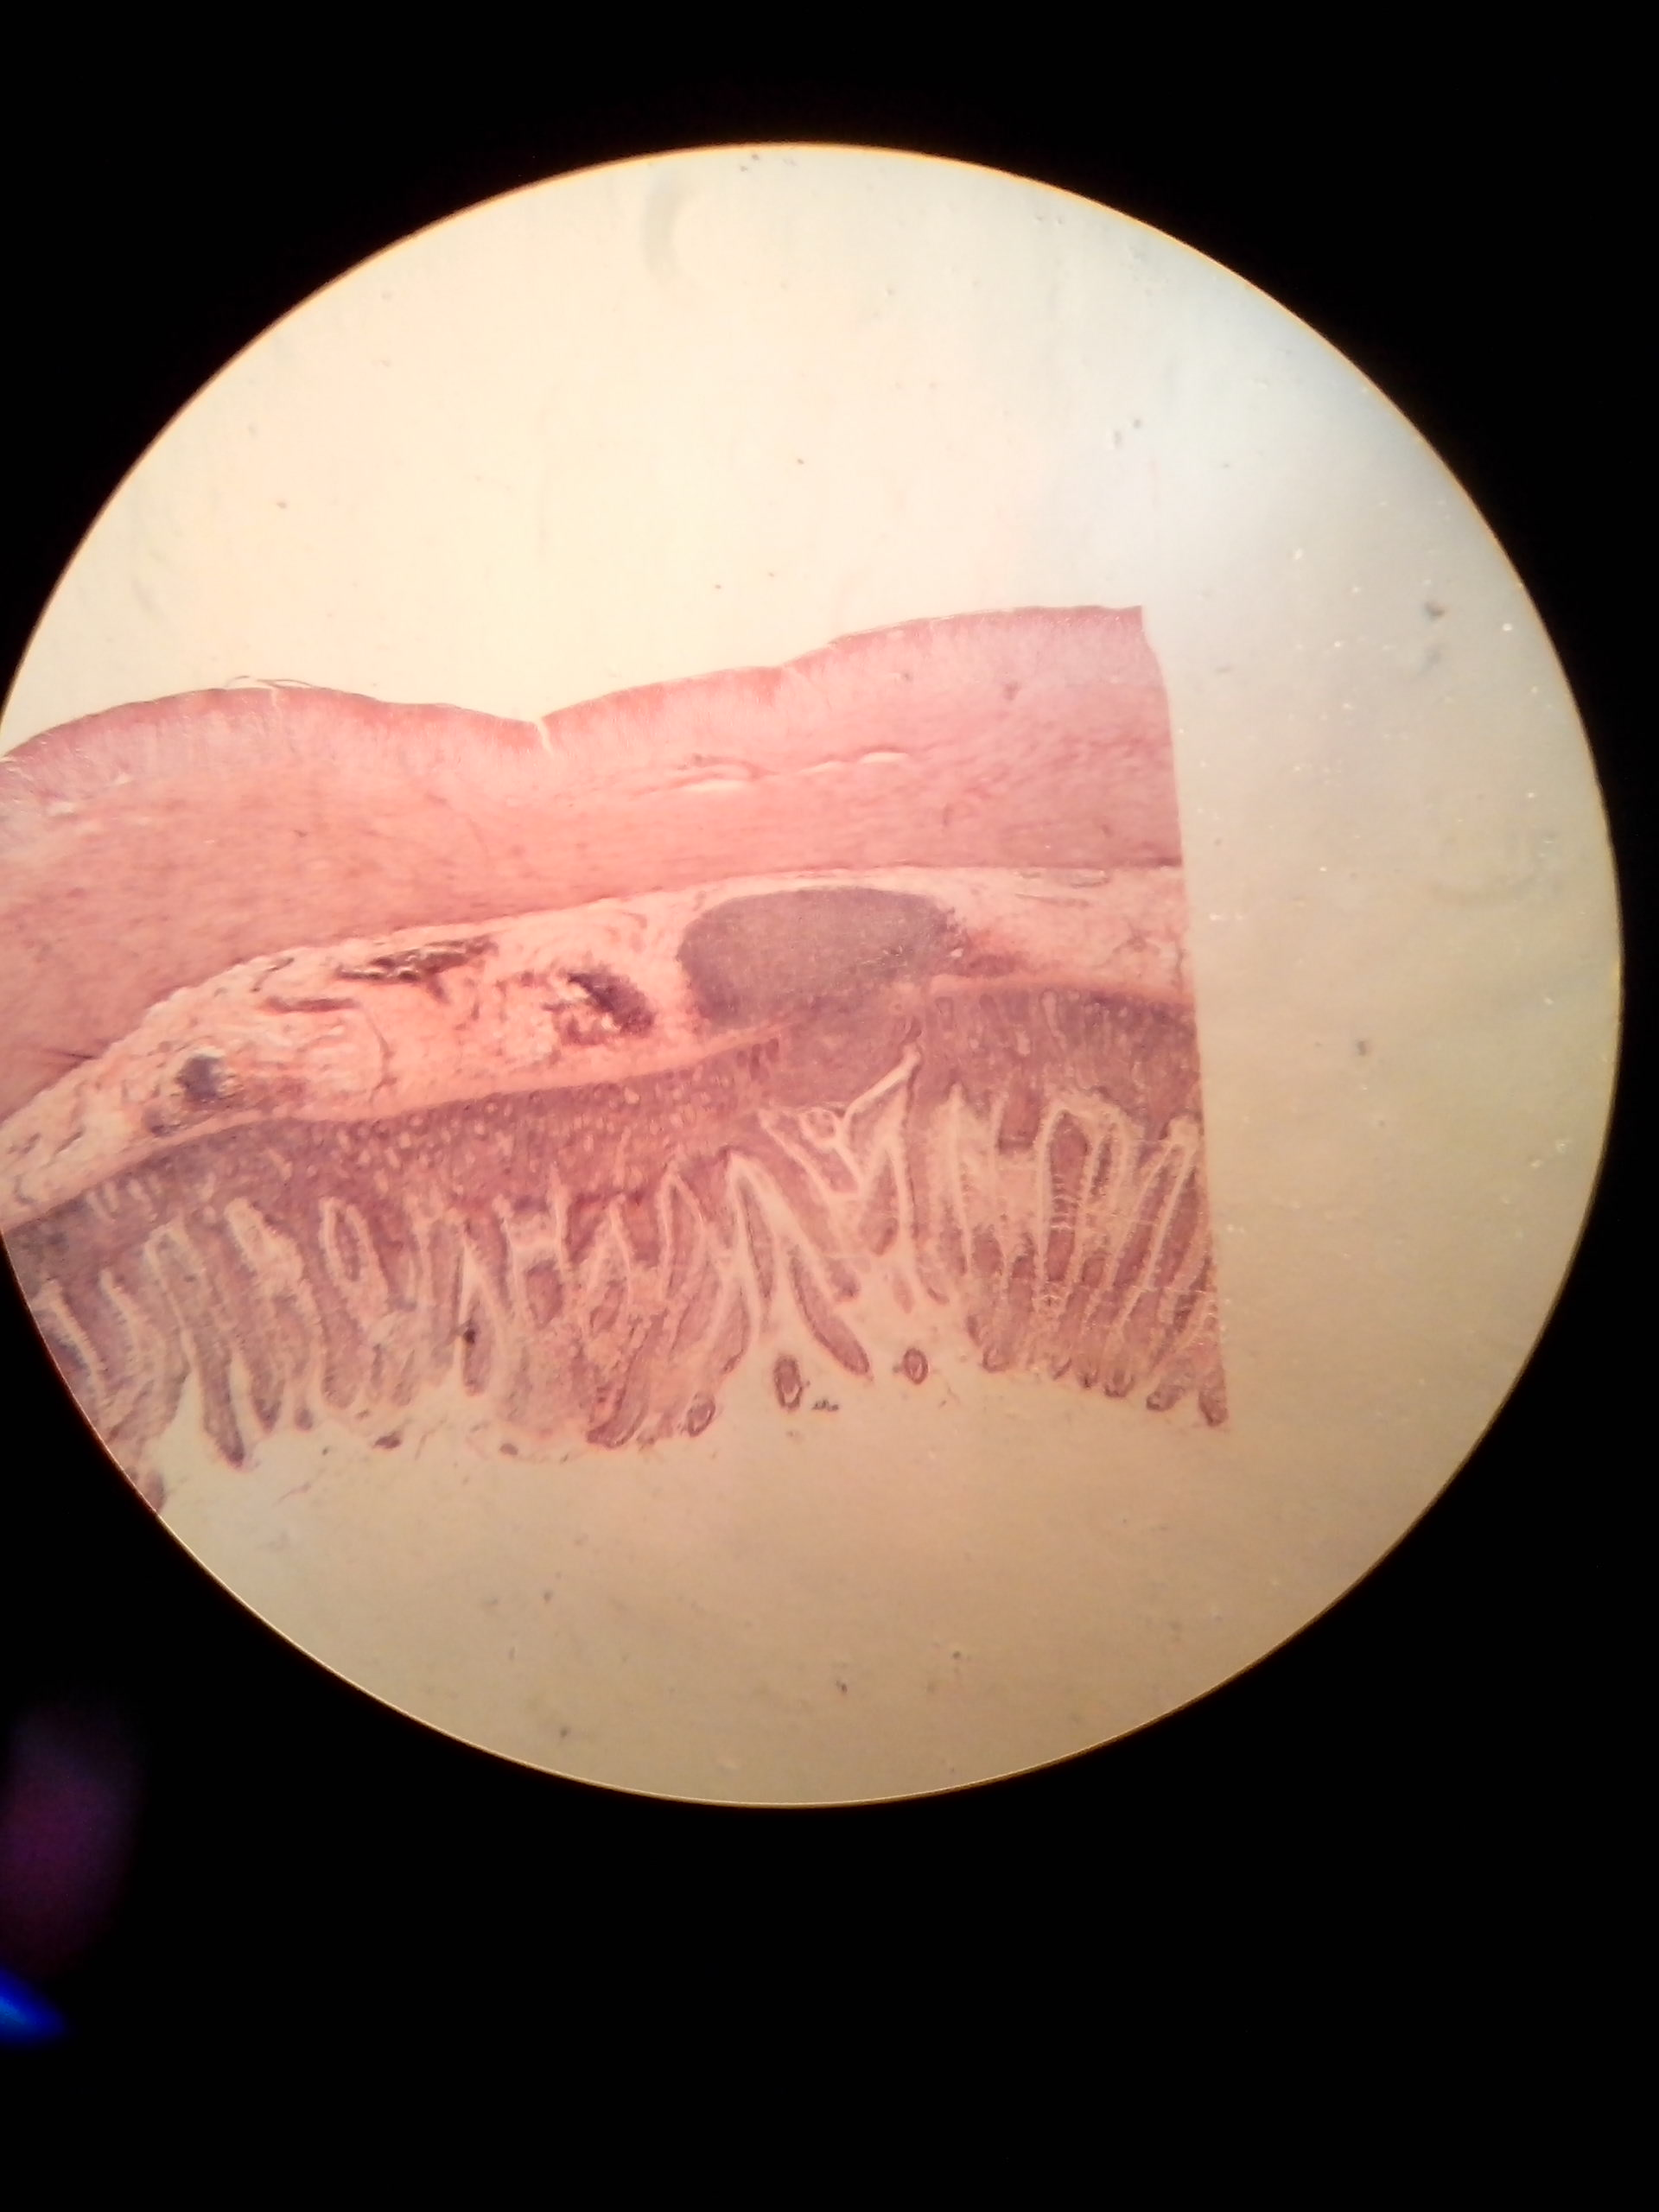
\includegraphics[width=1\textwidth]{../images/01_mammal_illeum.jpg}
		\caption{Objektiv 4x}
	\end{subfigure}
	\begin{subfigure}[b]{0.3\textwidth}
		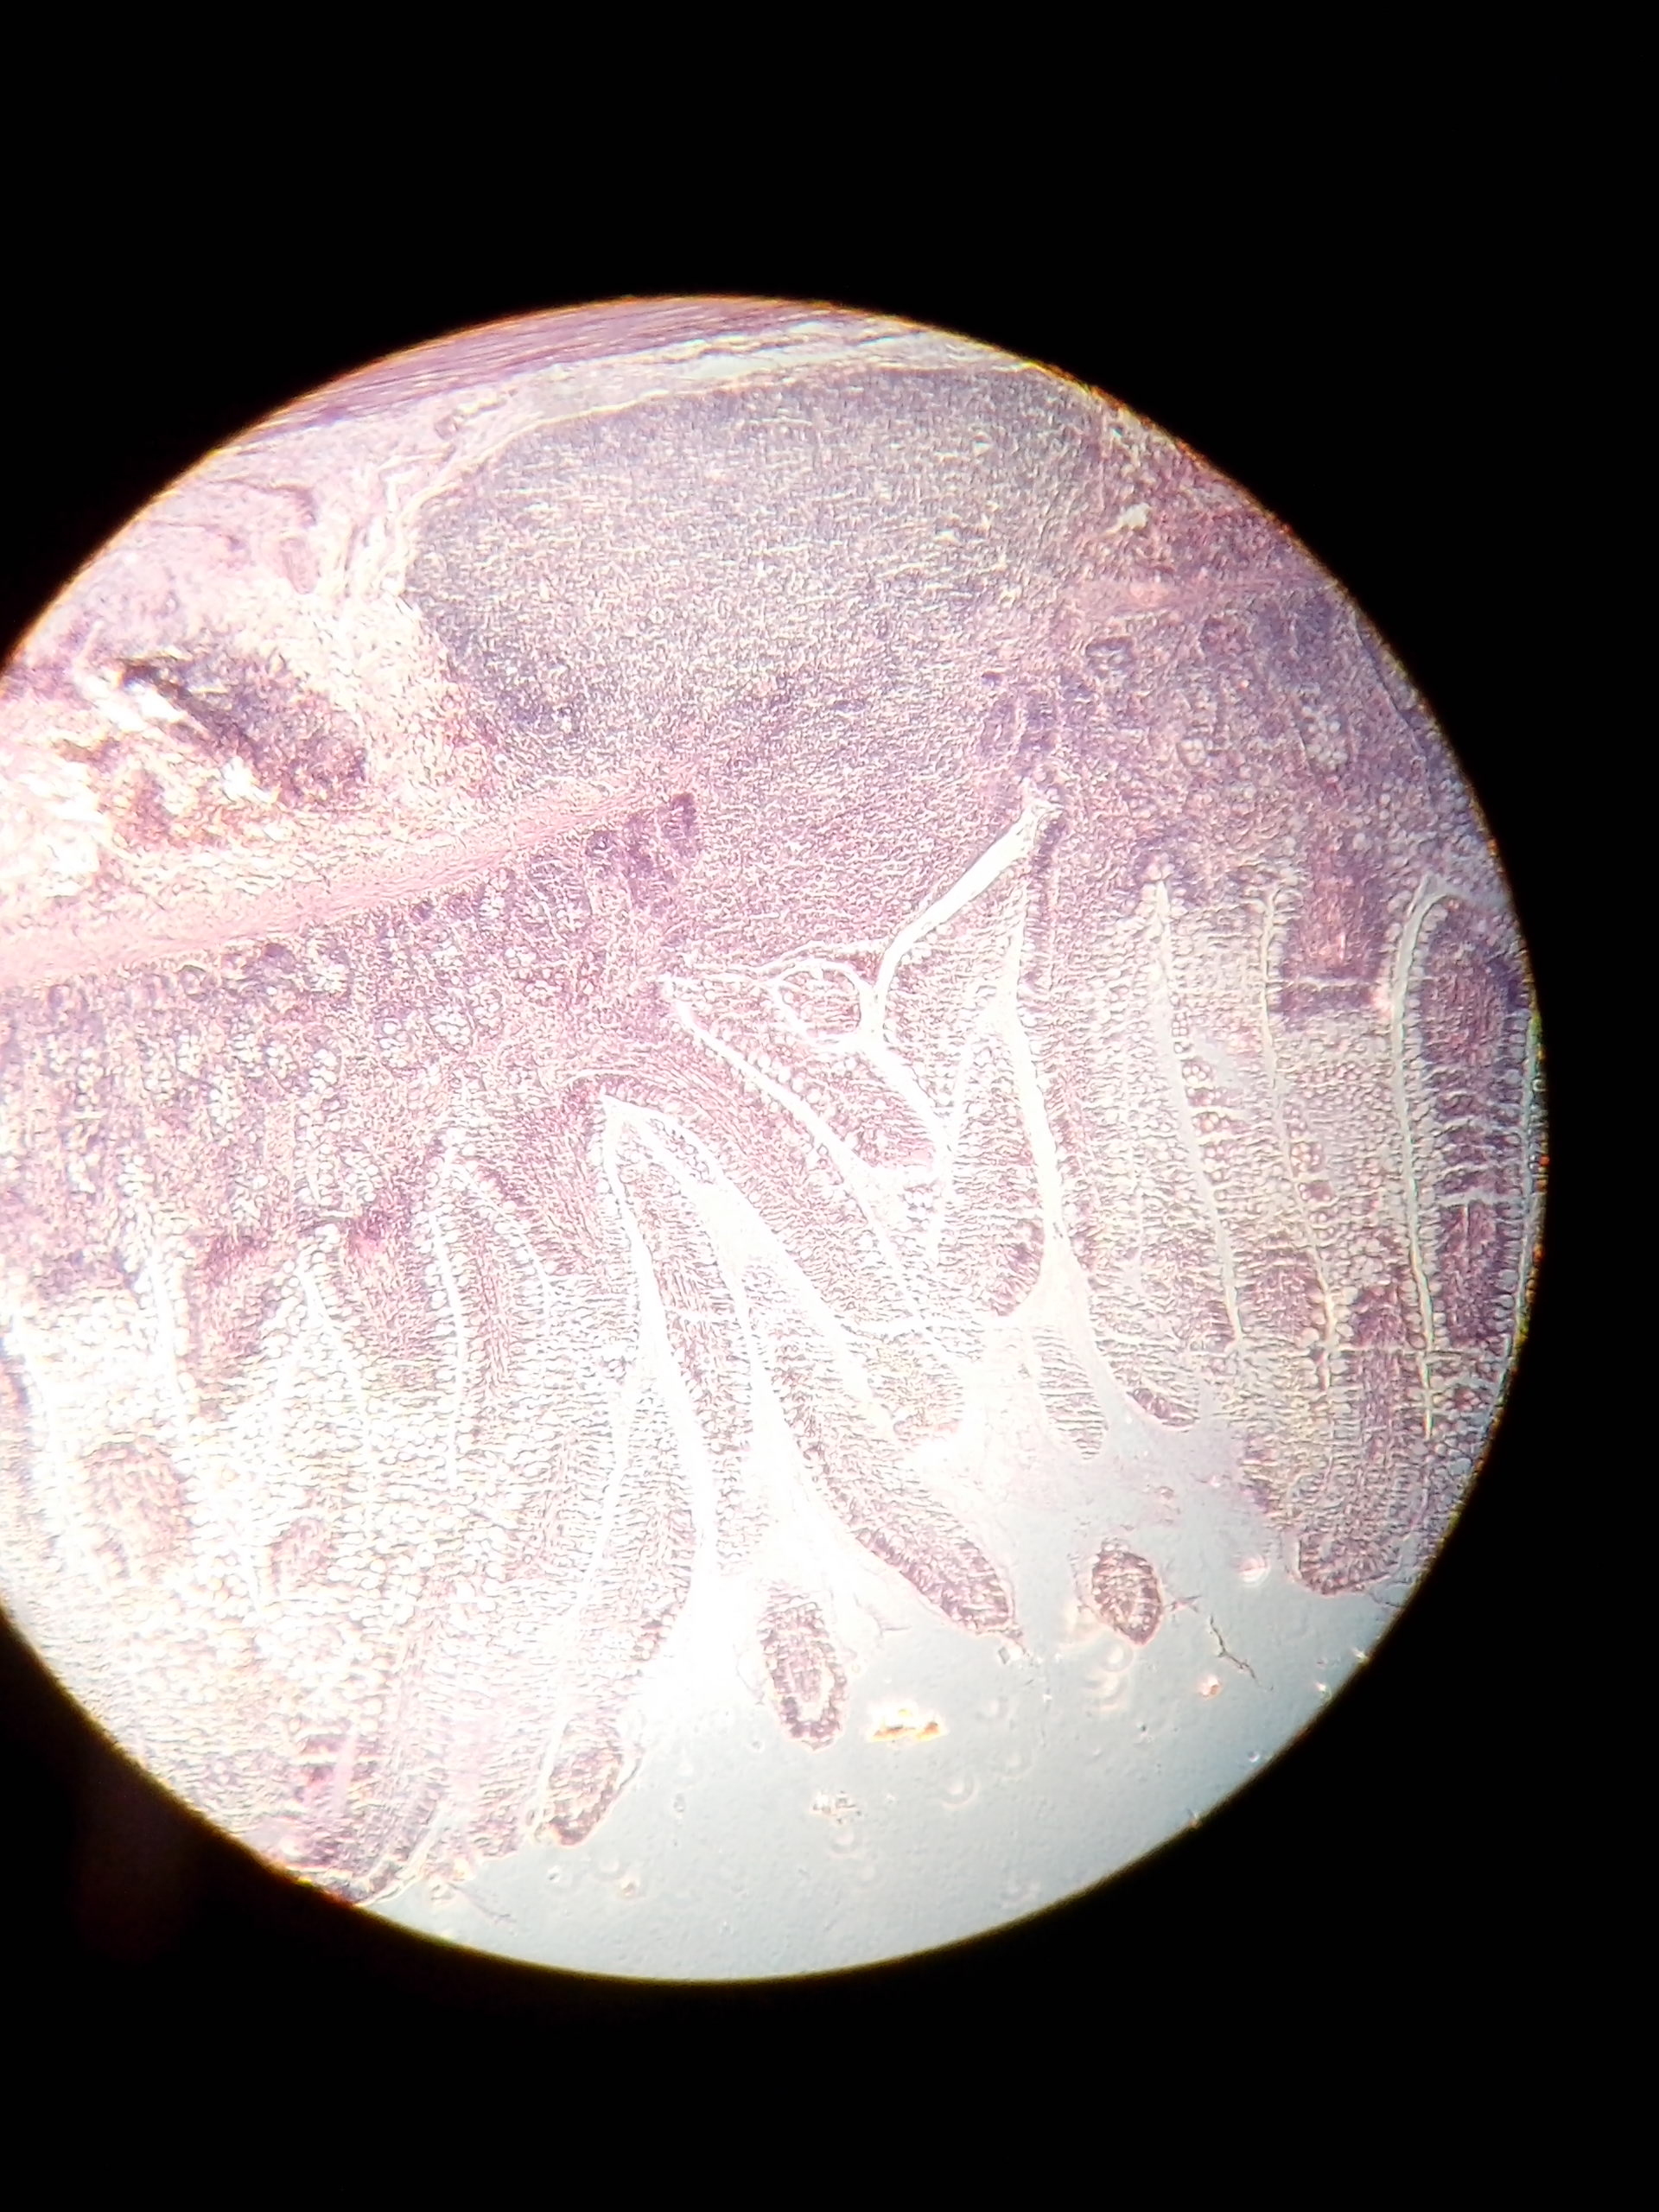
\includegraphics[width=1\textwidth]{../images/02_mammal_illeum.jpg}
		\caption{Objektiv 10x}
	\end{subfigure}
	\begin{subfigure}[b]{0.3\textwidth}
		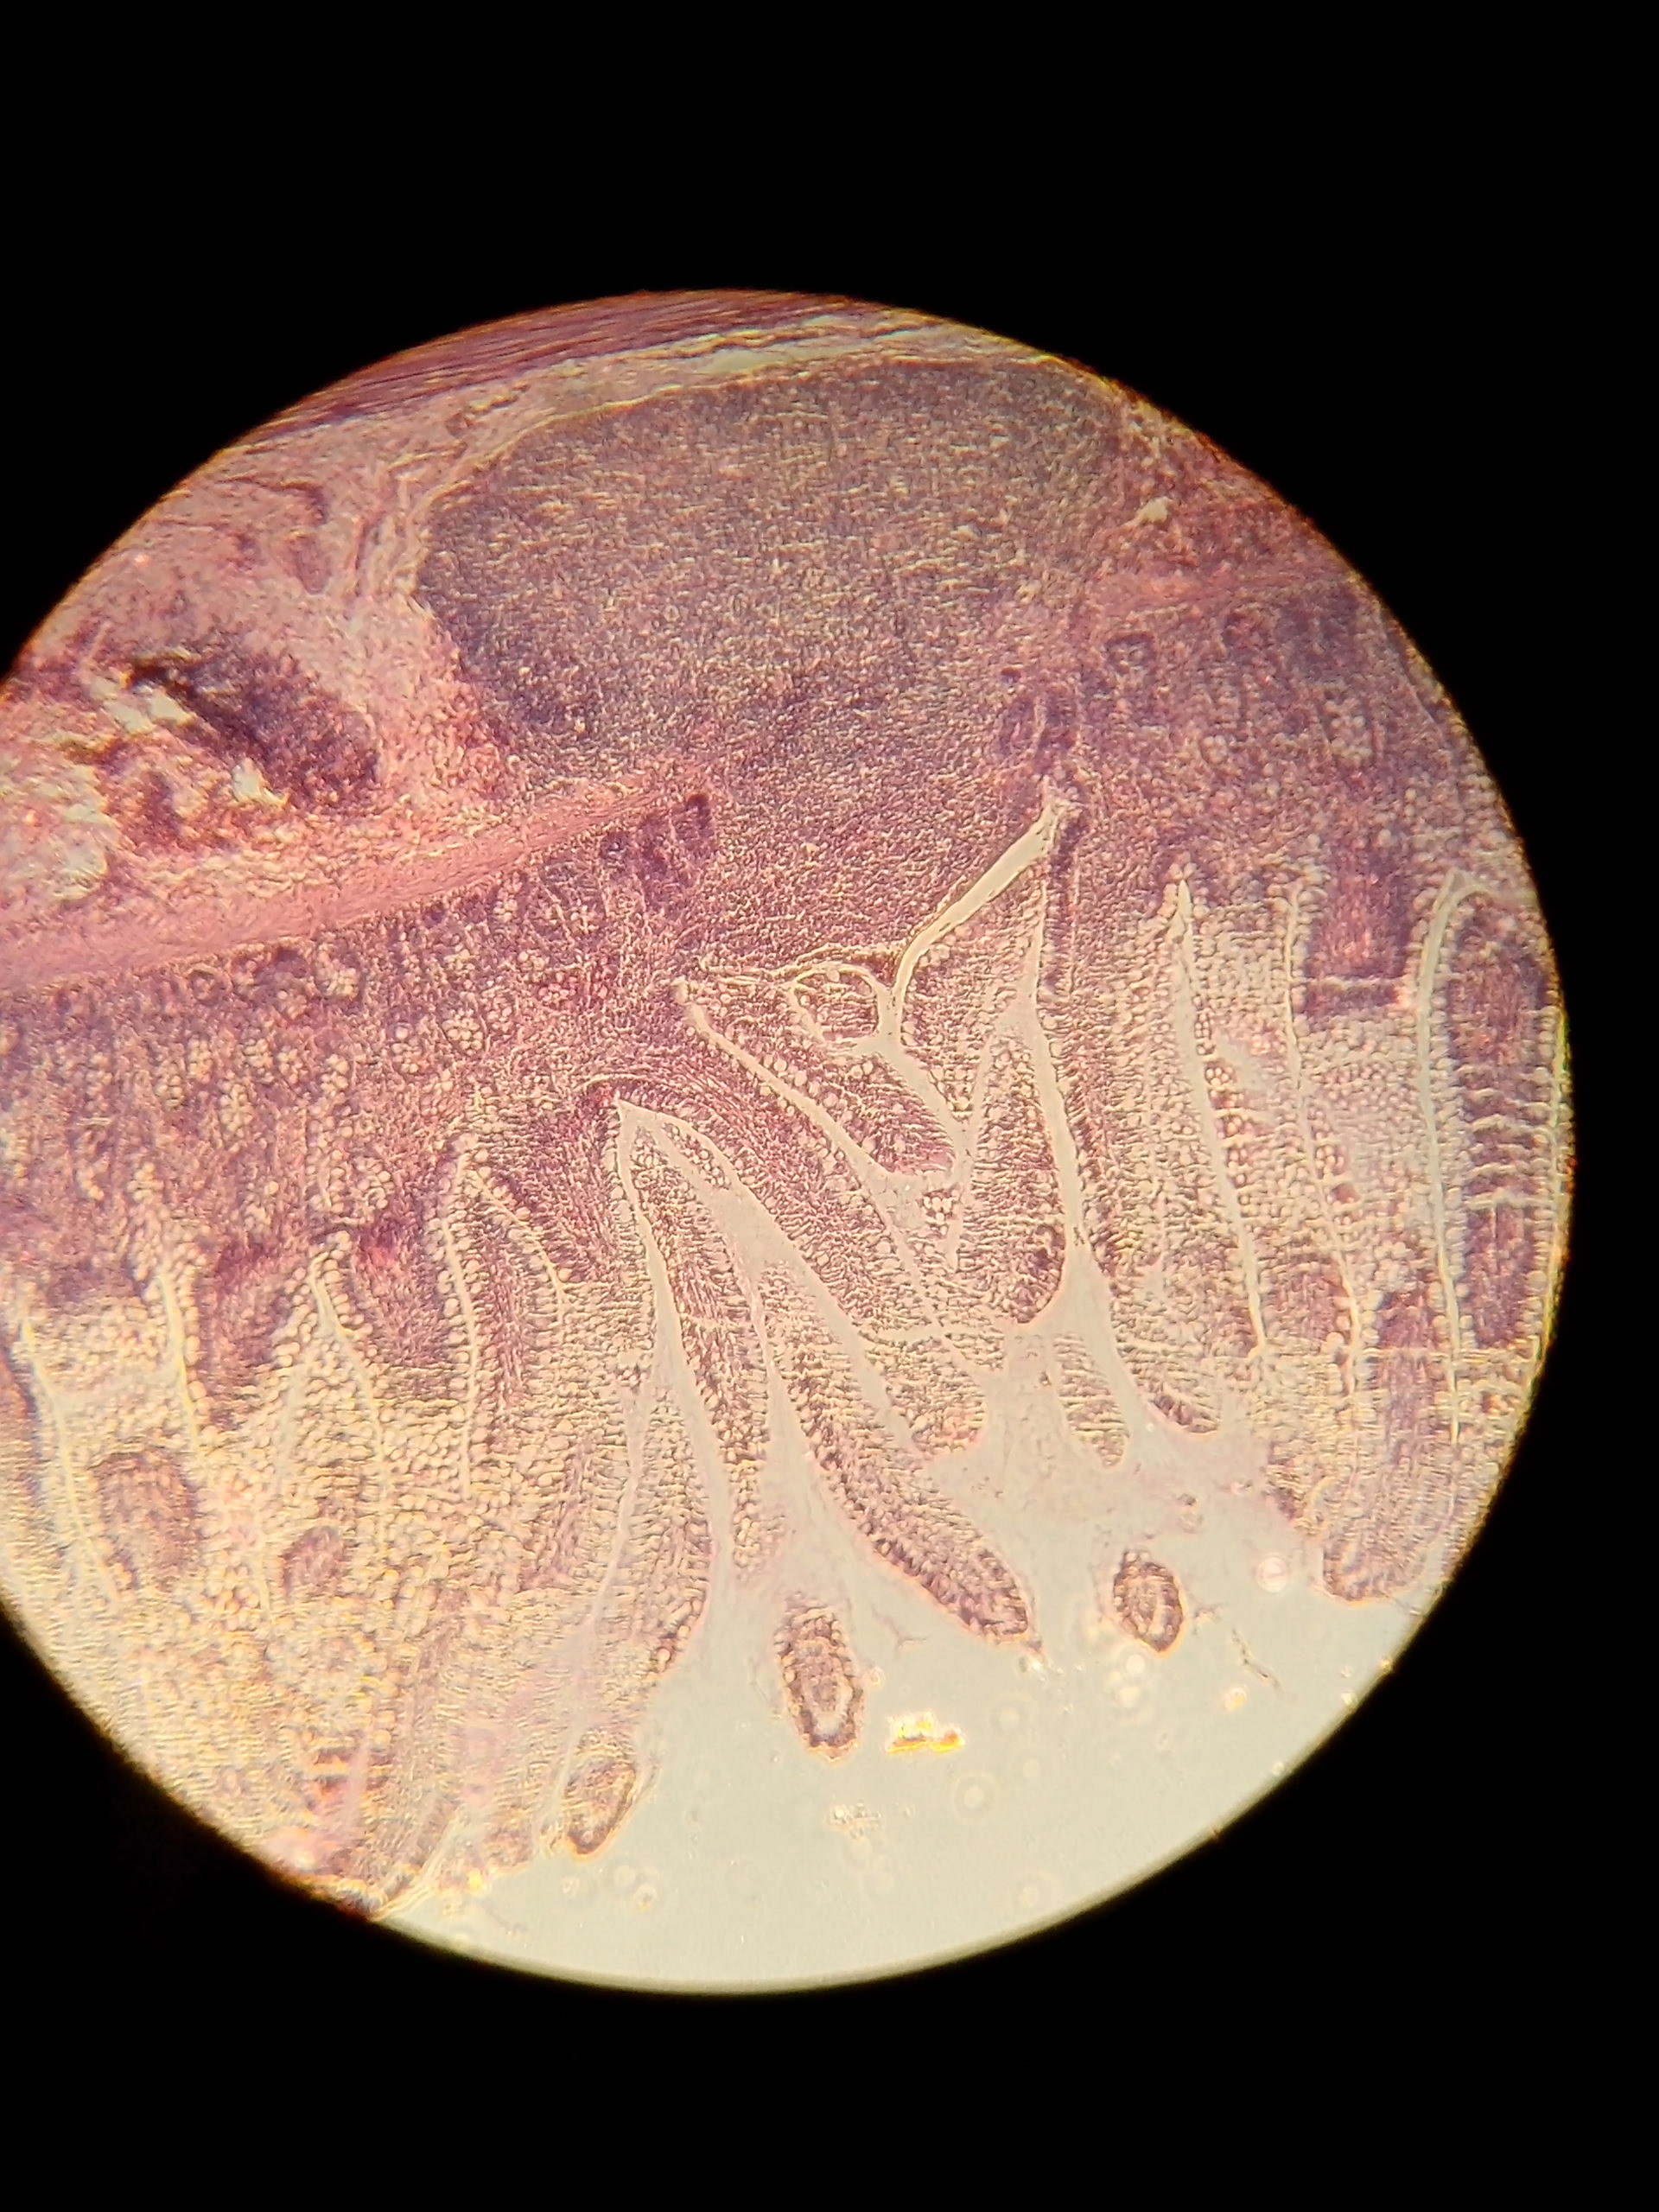
\includegraphics[width=1\textwidth]{../images/03_mammal_illeum.jpg}
		\caption{Objektiv 10x}
	\end{subfigure}

	\begin{subfigure}[b]{0.3\textwidth}
		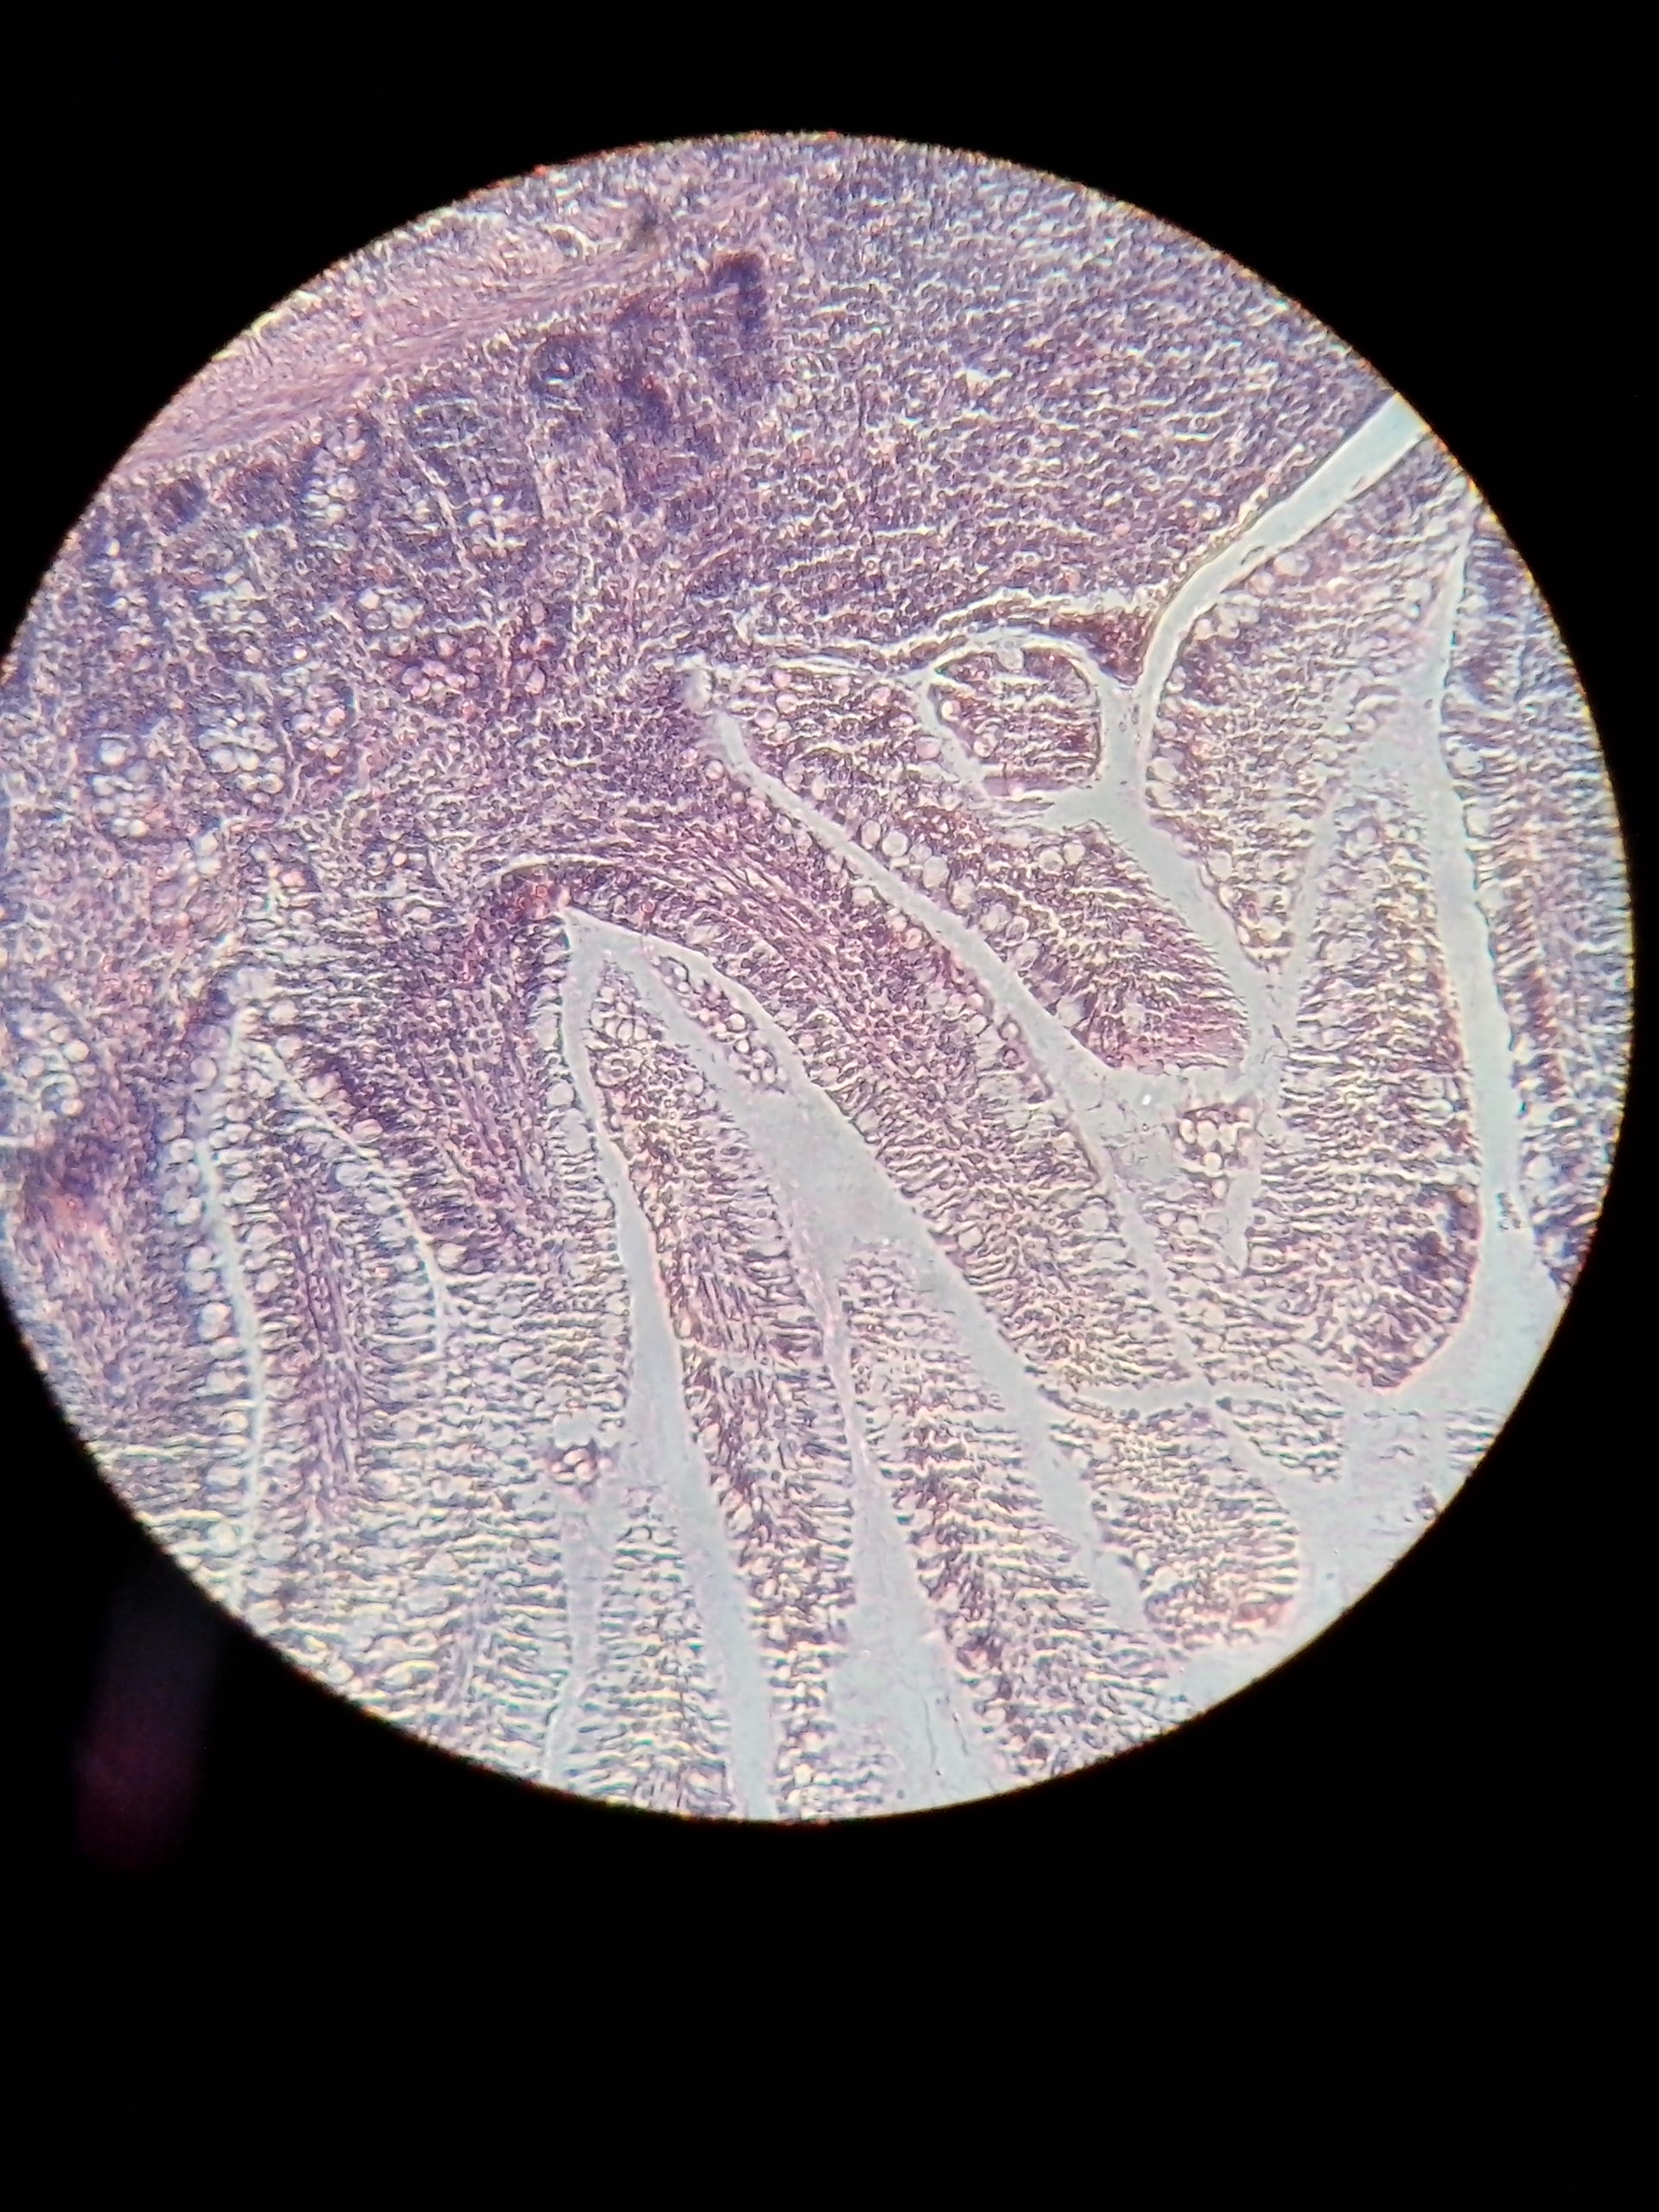
\includegraphics[width=1\textwidth]{../images/04_mammal_illeum.jpg}
		\caption{Objektiv 20x}
	\end{subfigure}
	\begin{subfigure}[b]{0.3\textwidth}
		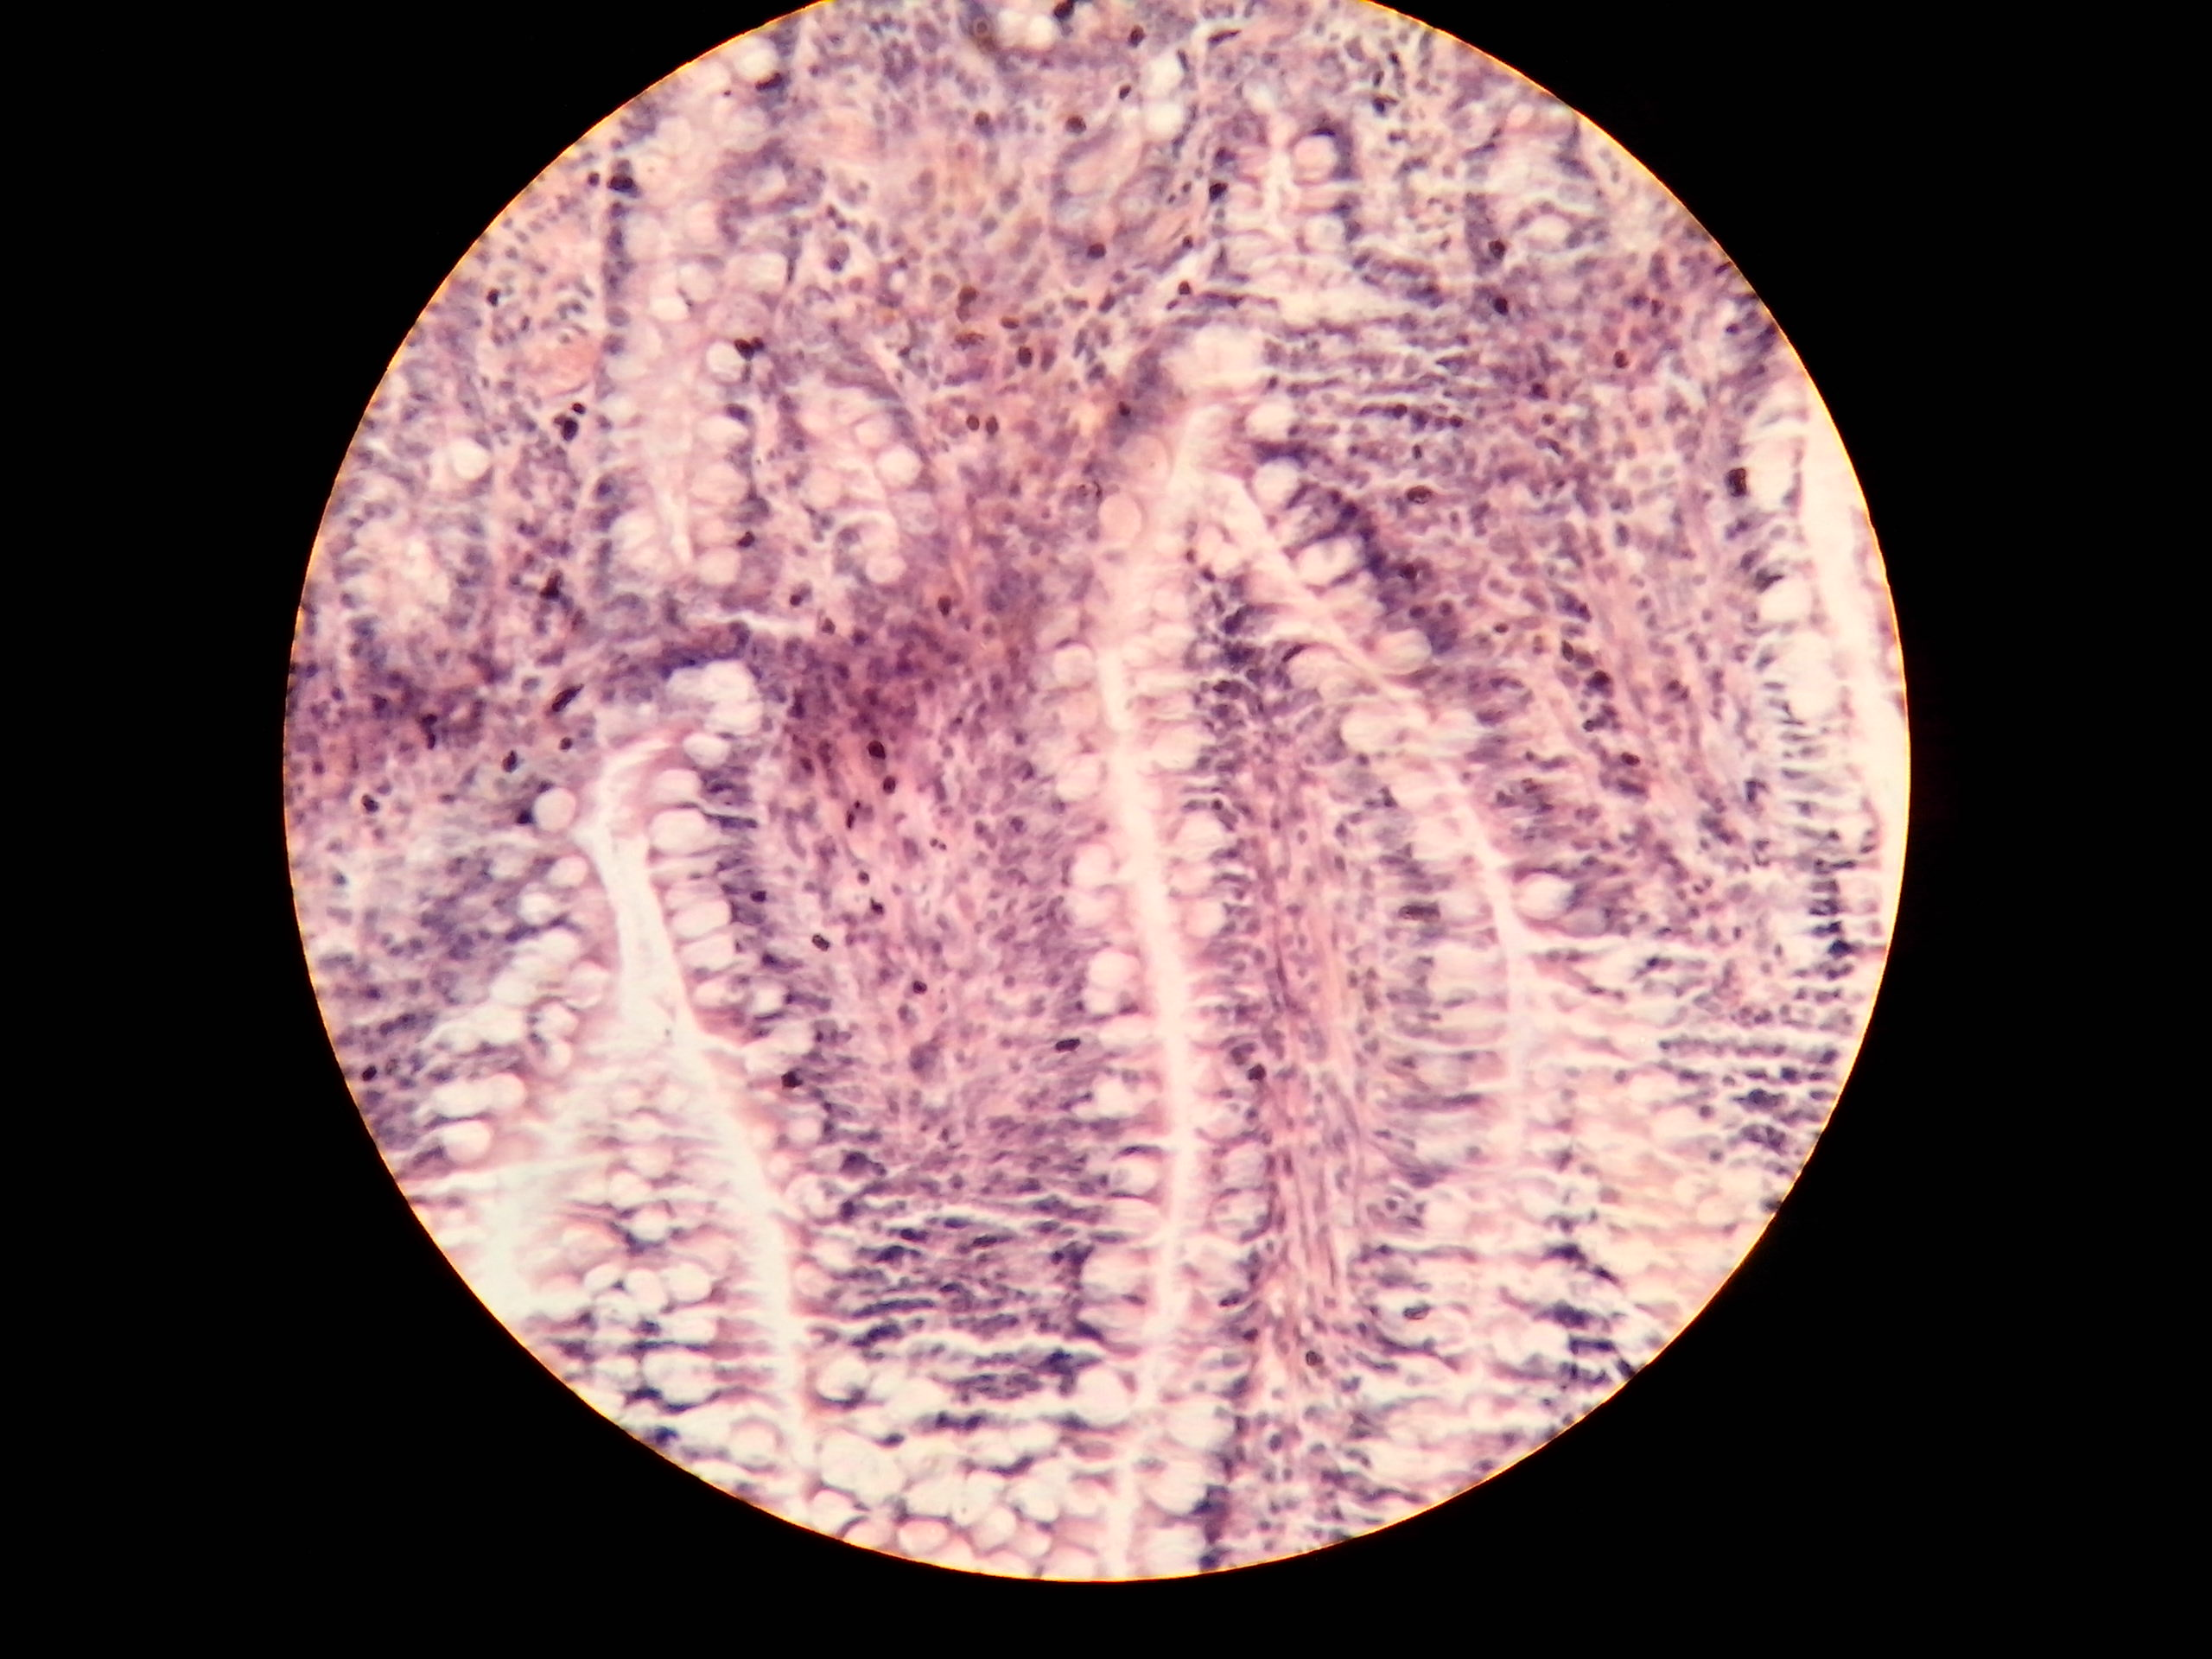
\includegraphics[angle=270, width=1\textwidth]{../images/05_mammal_illeum.jpg}
		\caption{Objektiv 40x}
	\end{subfigure}
	\begin{subfigure}[b]{0.3\textwidth}
		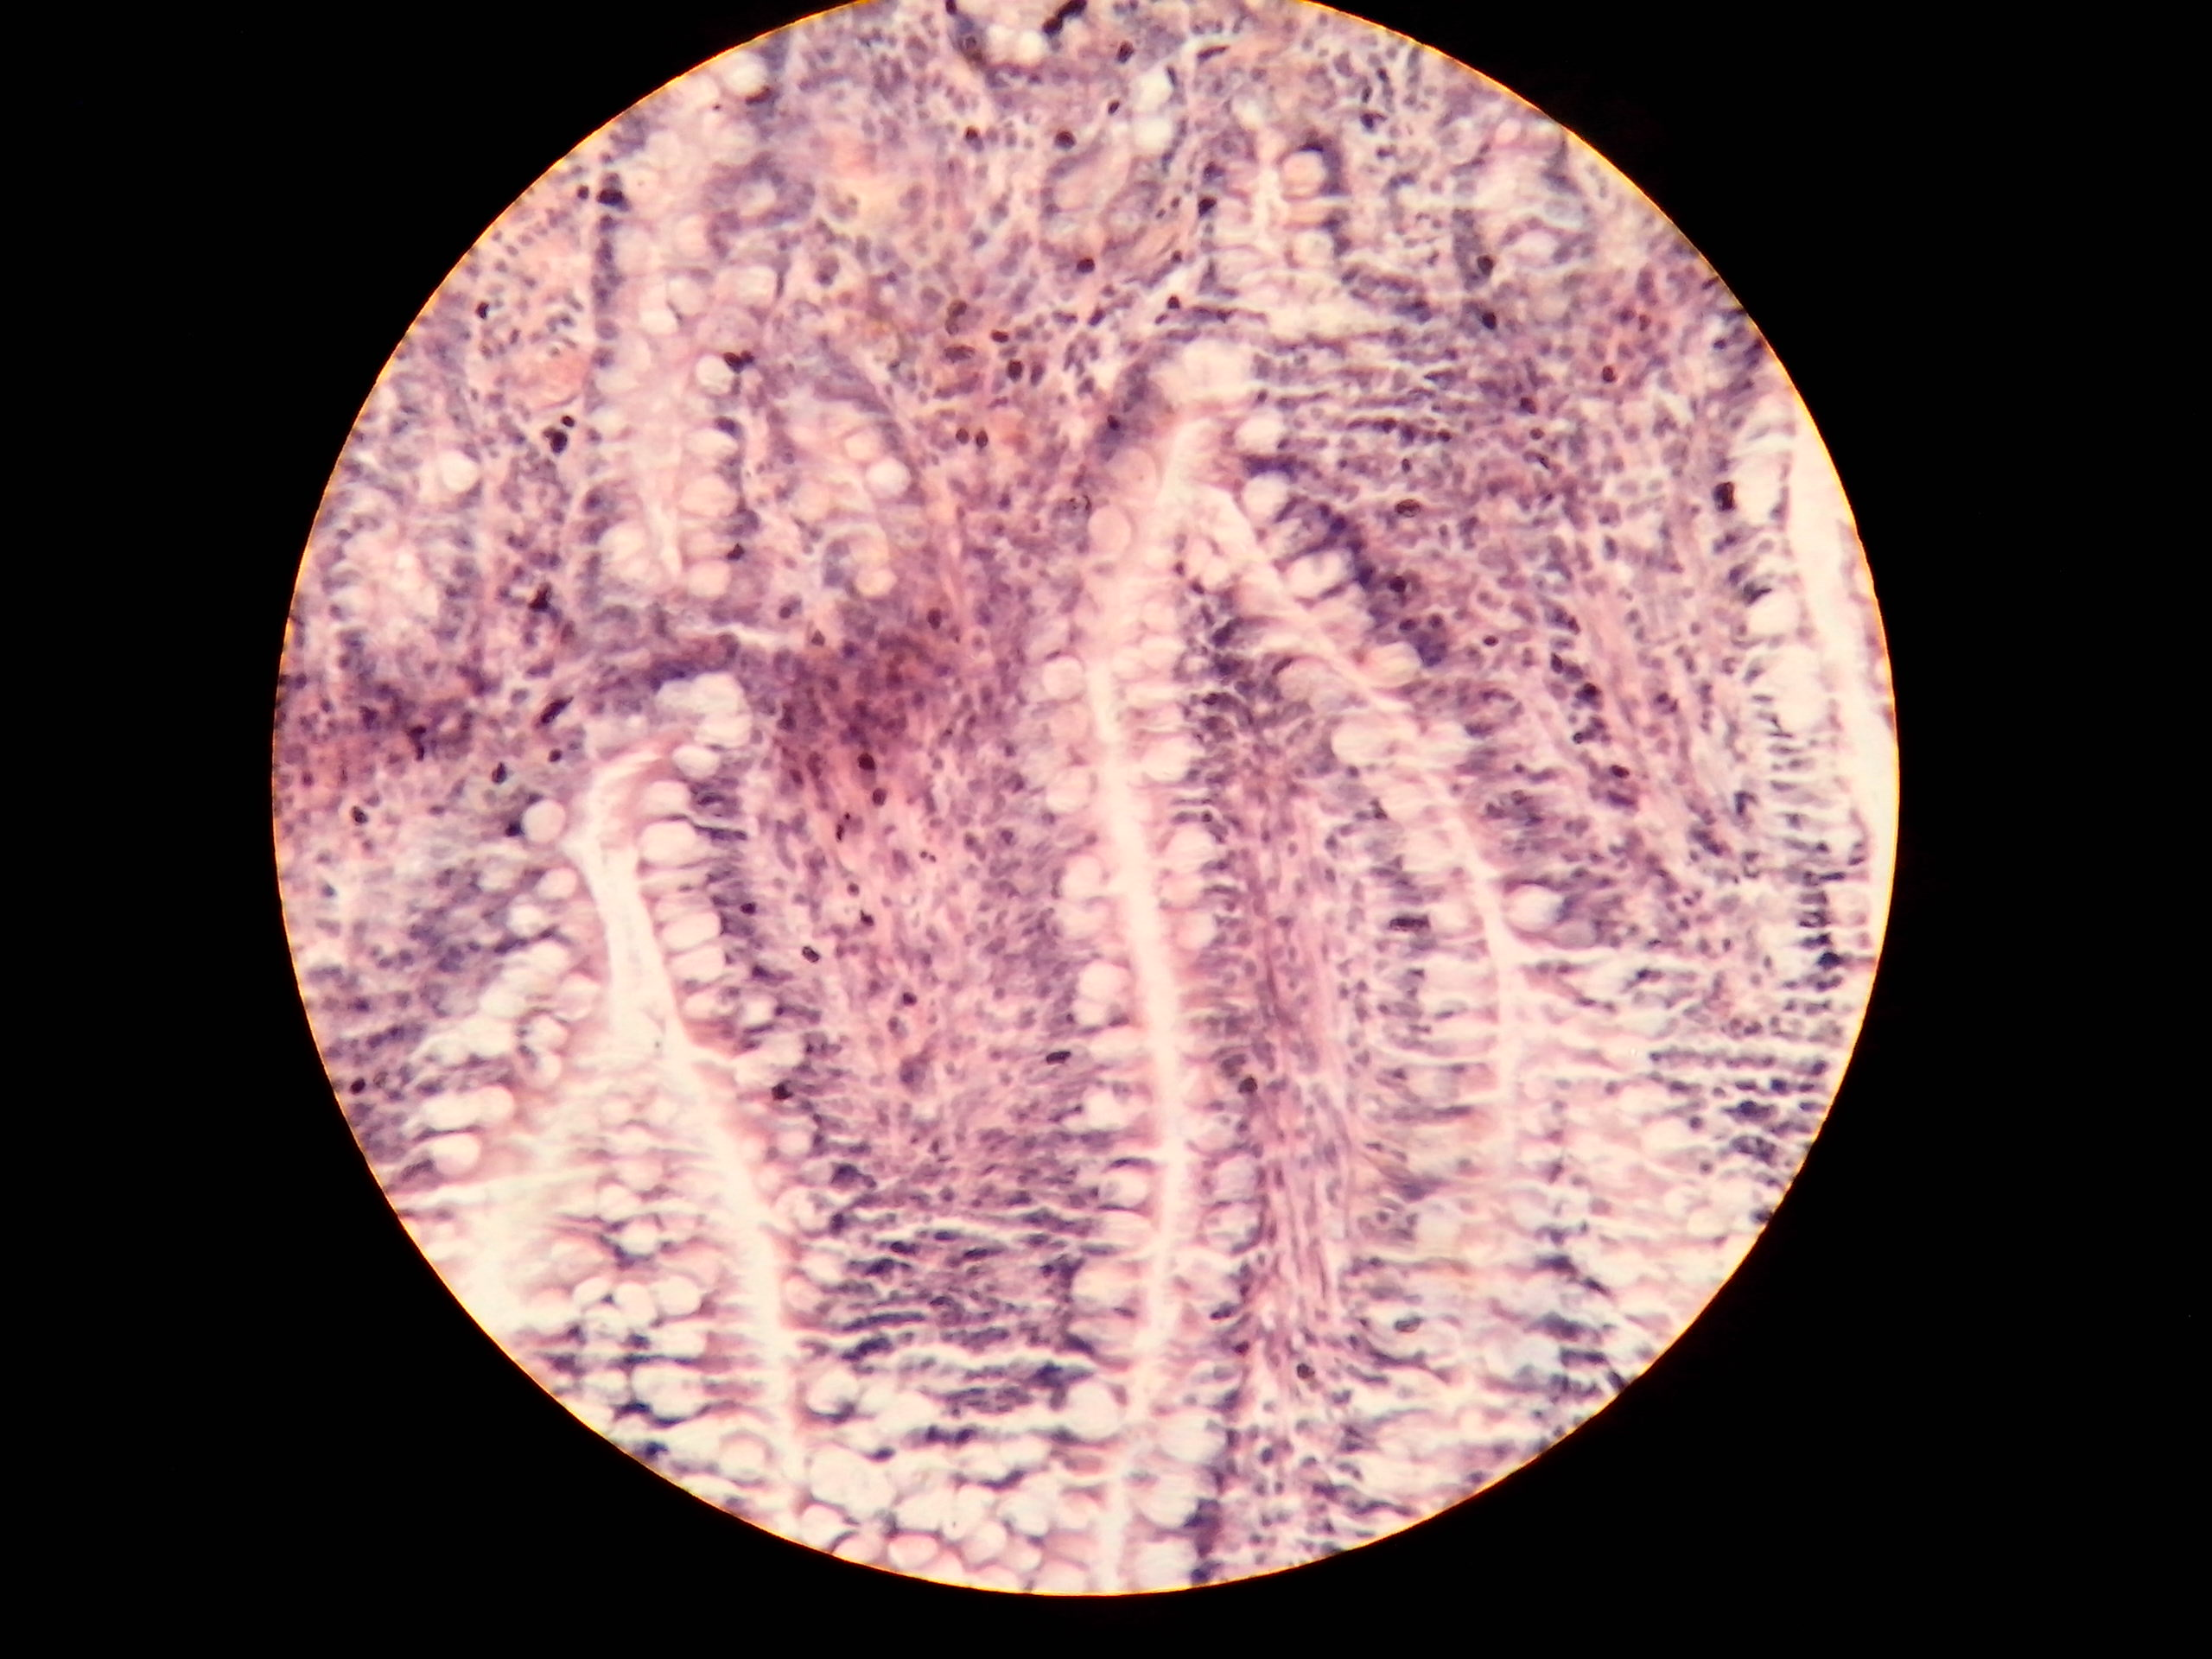
\includegraphics[angle=270, width=1\textwidth]{../images/06_mammal_illeum.jpg}
		\caption{Objektiv 40x}
	\end{subfigure}
	\caption{Aufzeichnungen der Lichtmikorskopischen Darstellungen der
		Dünndarmproben}
\end{figure}

\subsubsection{Kommentar}

\newpage
\subsection{Menschliche Leber}

\subsubsection{Proben}
\begin{table}[h!]
	\centering
	\begin{tabular}{l l}
		Bezeichnung	& Human liver \\
		Probe 		& 31-5388
	\end{tabular}
\end{table}

\subsubsection{Aufzeichnungen}
\begin{figure}[h!]
	\centering
	\begin{subfigure}[b]{0.3\textwidth}
		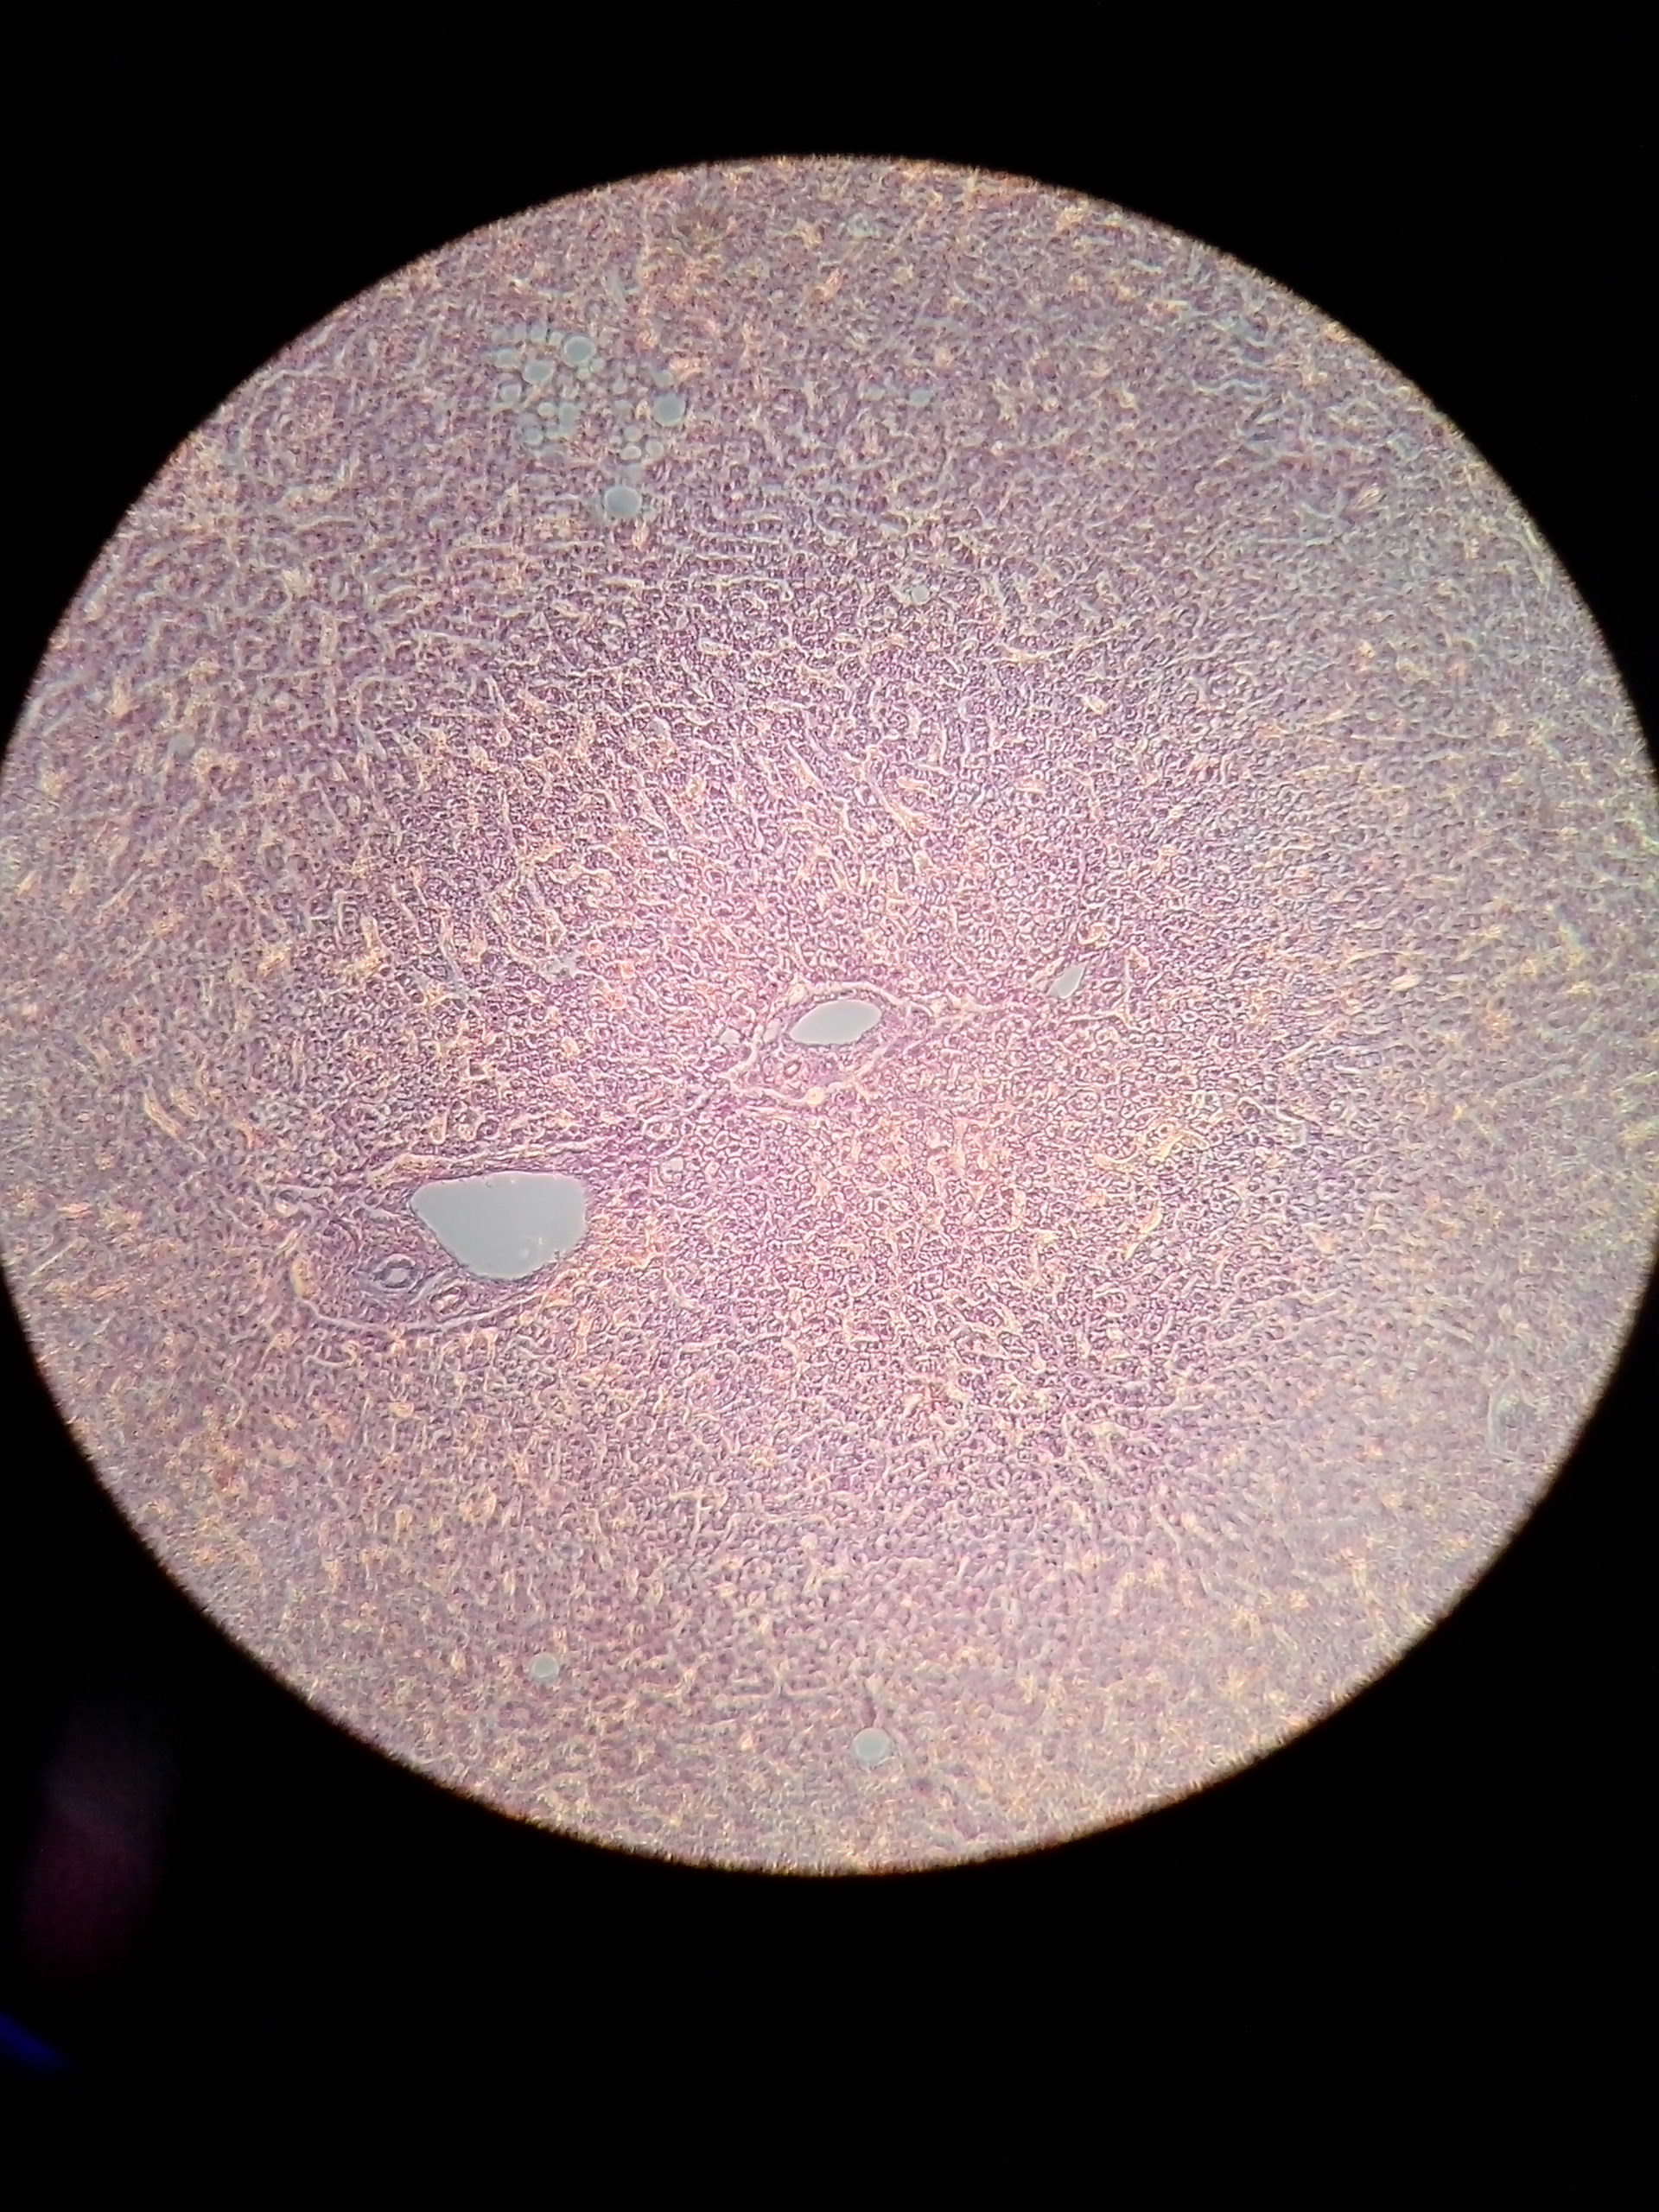
\includegraphics[width=1\textwidth]{../images/01_human_liver.jpg}
		\caption{Objektiv 10x}
	\end{subfigure}
	\begin{subfigure}[b]{0.3\textwidth}
		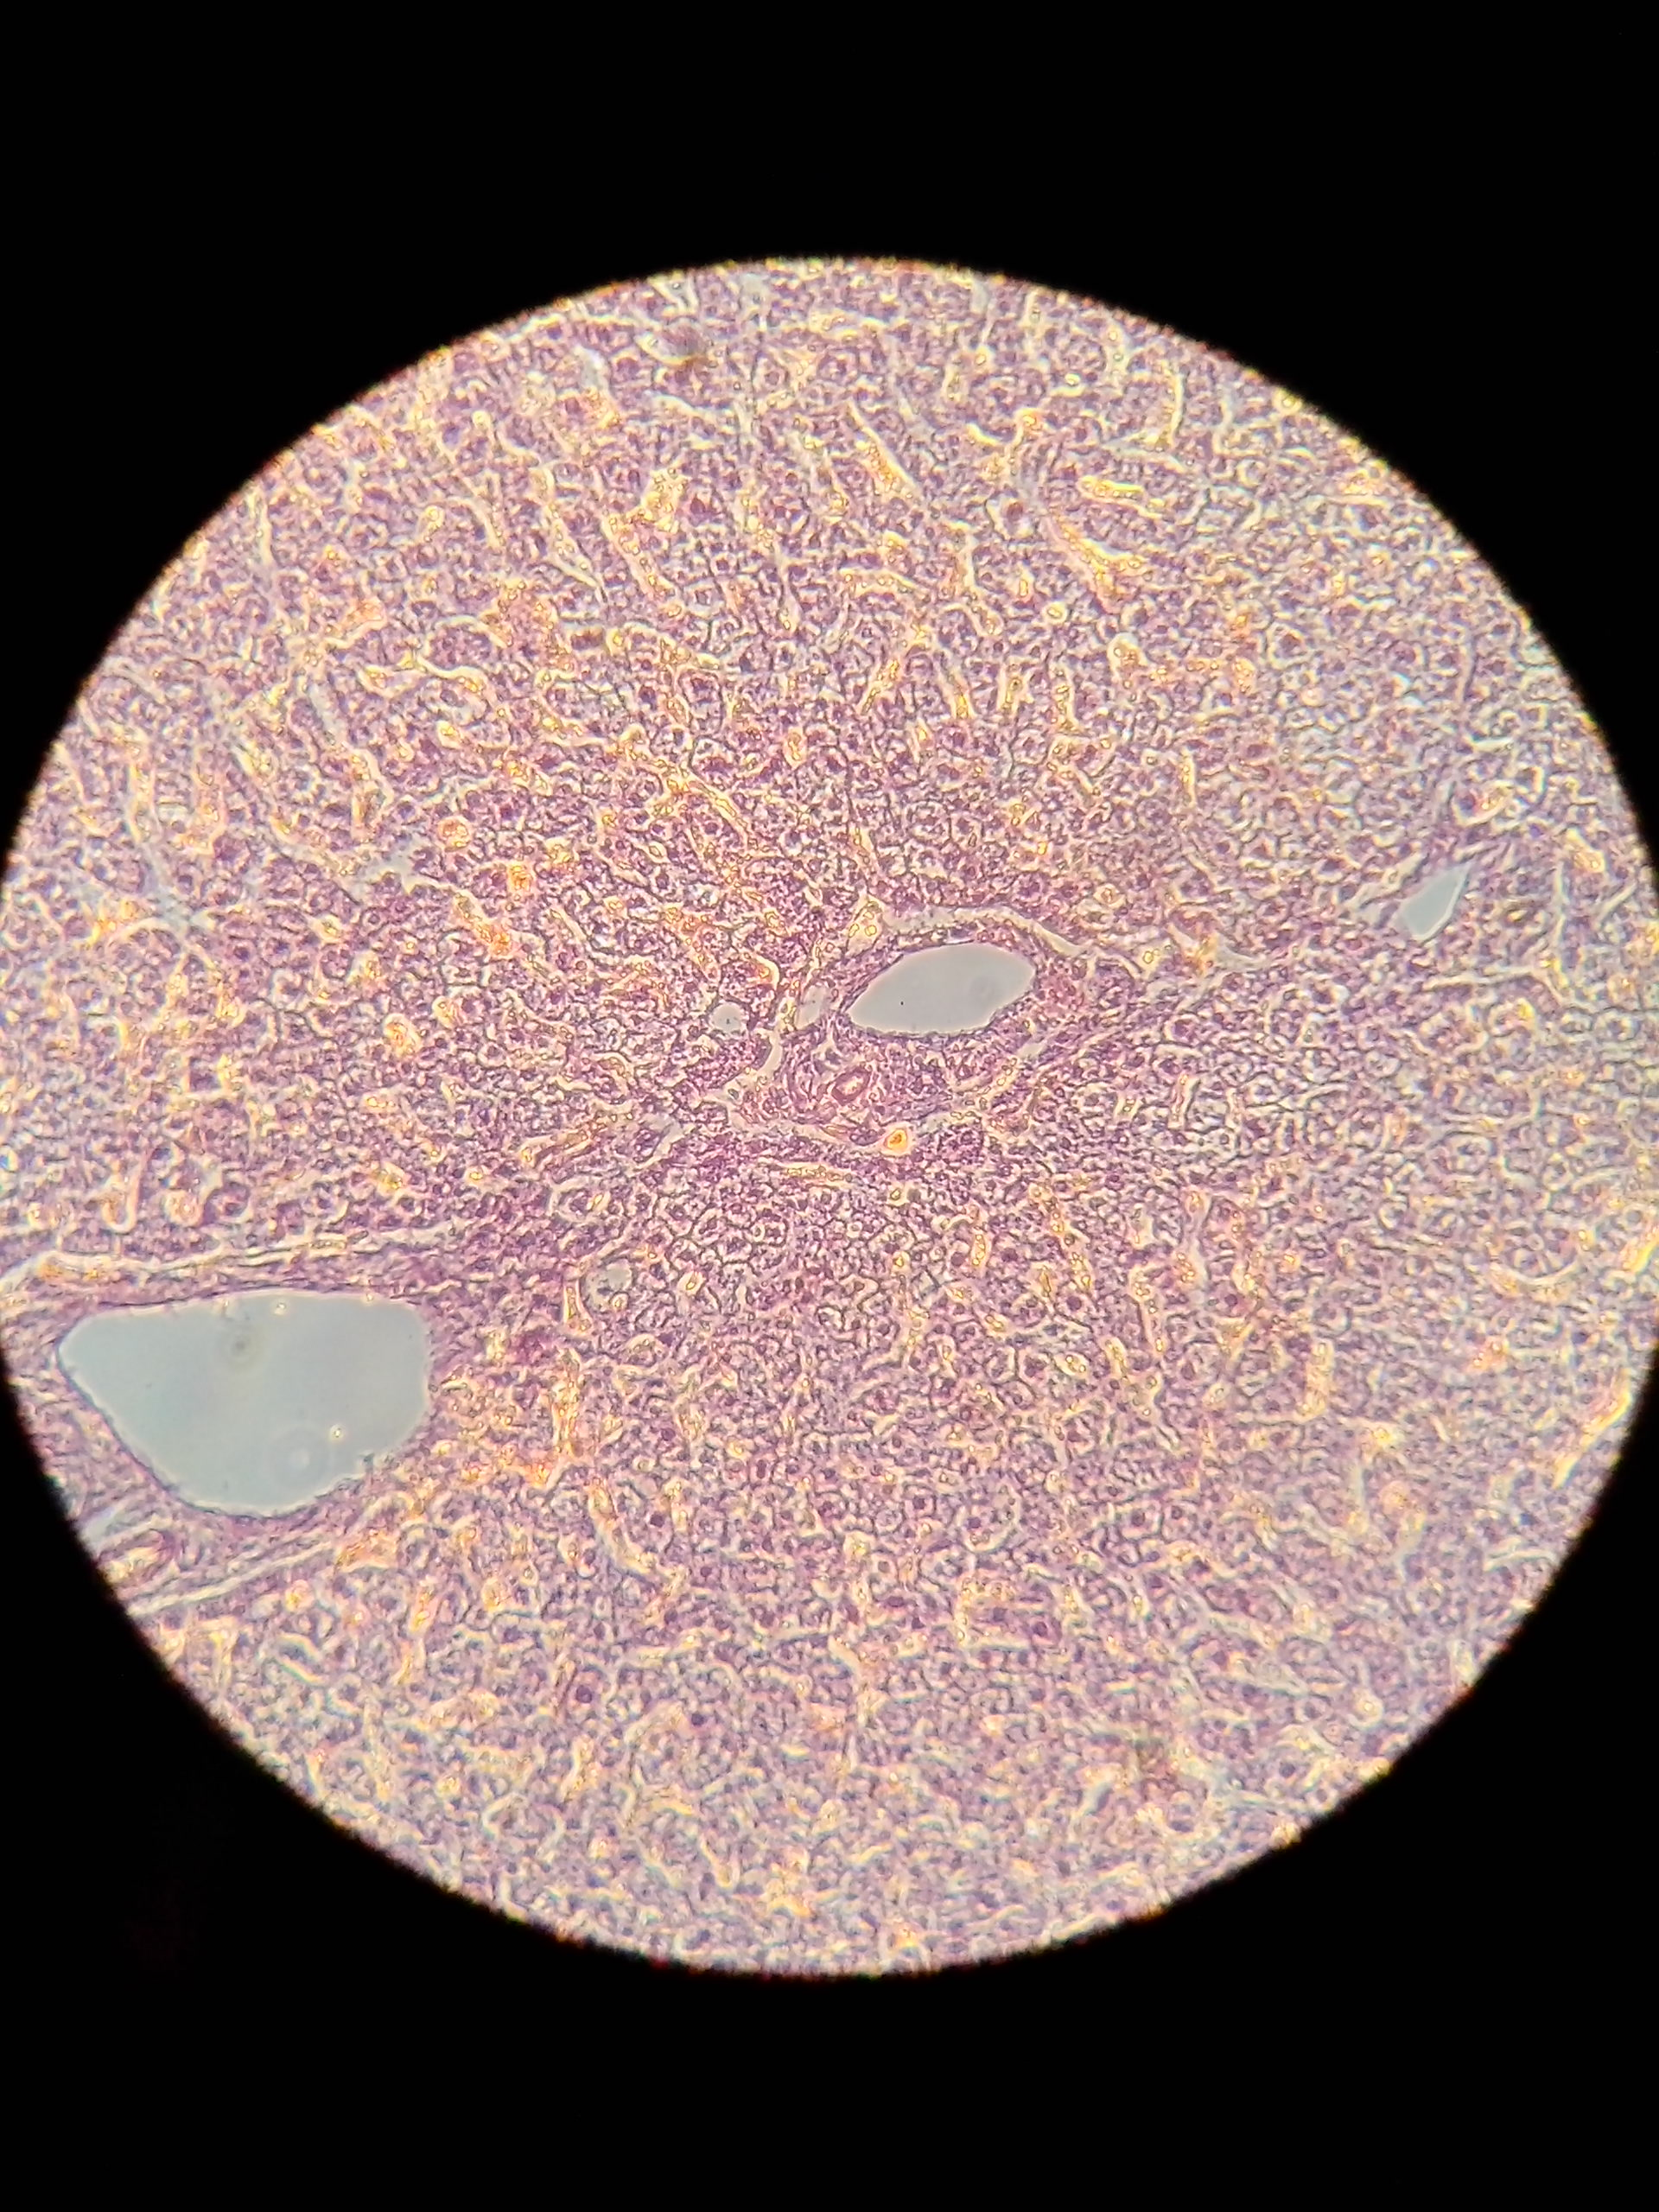
\includegraphics[width=1\textwidth]{../images/04_human_liver.jpg}
		\caption{Objektiv 20x}
	\end{subfigure}
	\begin{subfigure}[b]{0.3\textwidth}
		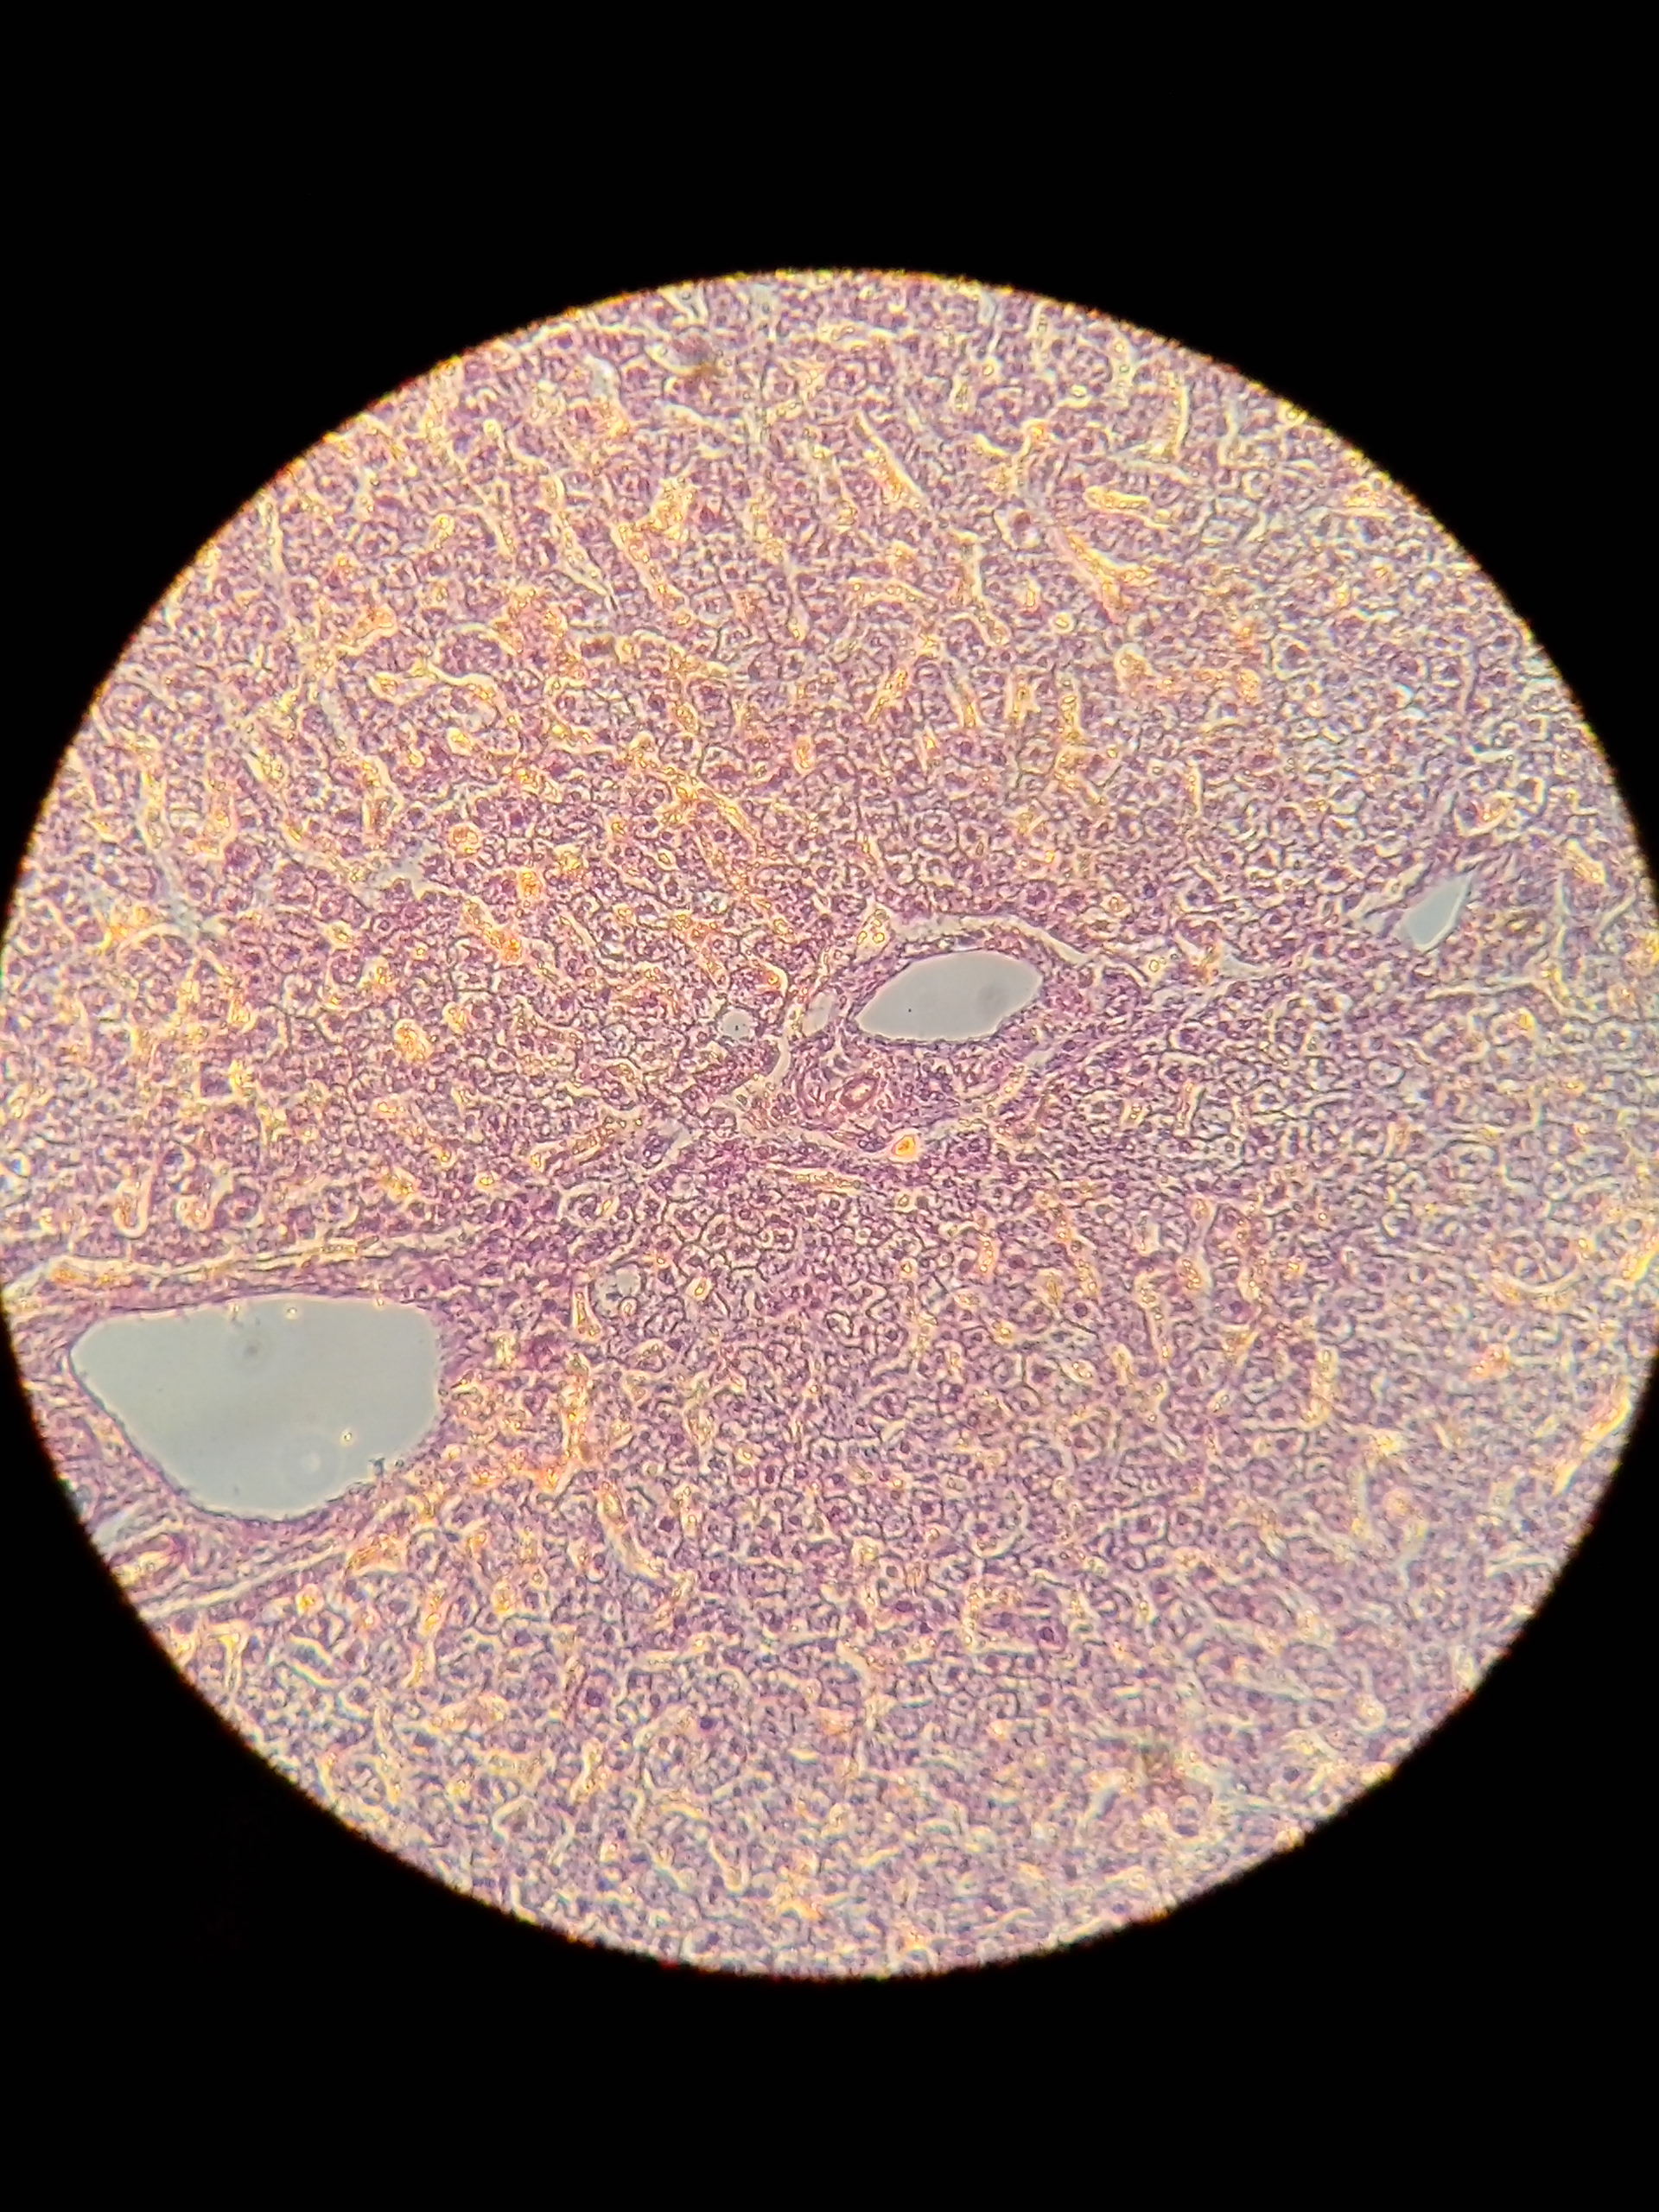
\includegraphics[width=1\textwidth]{../images/05_human_liver.jpg}
		\caption{Objektiv 20x}
	\end{subfigure}

	\begin{subfigure}[b]{0.3\textwidth}
		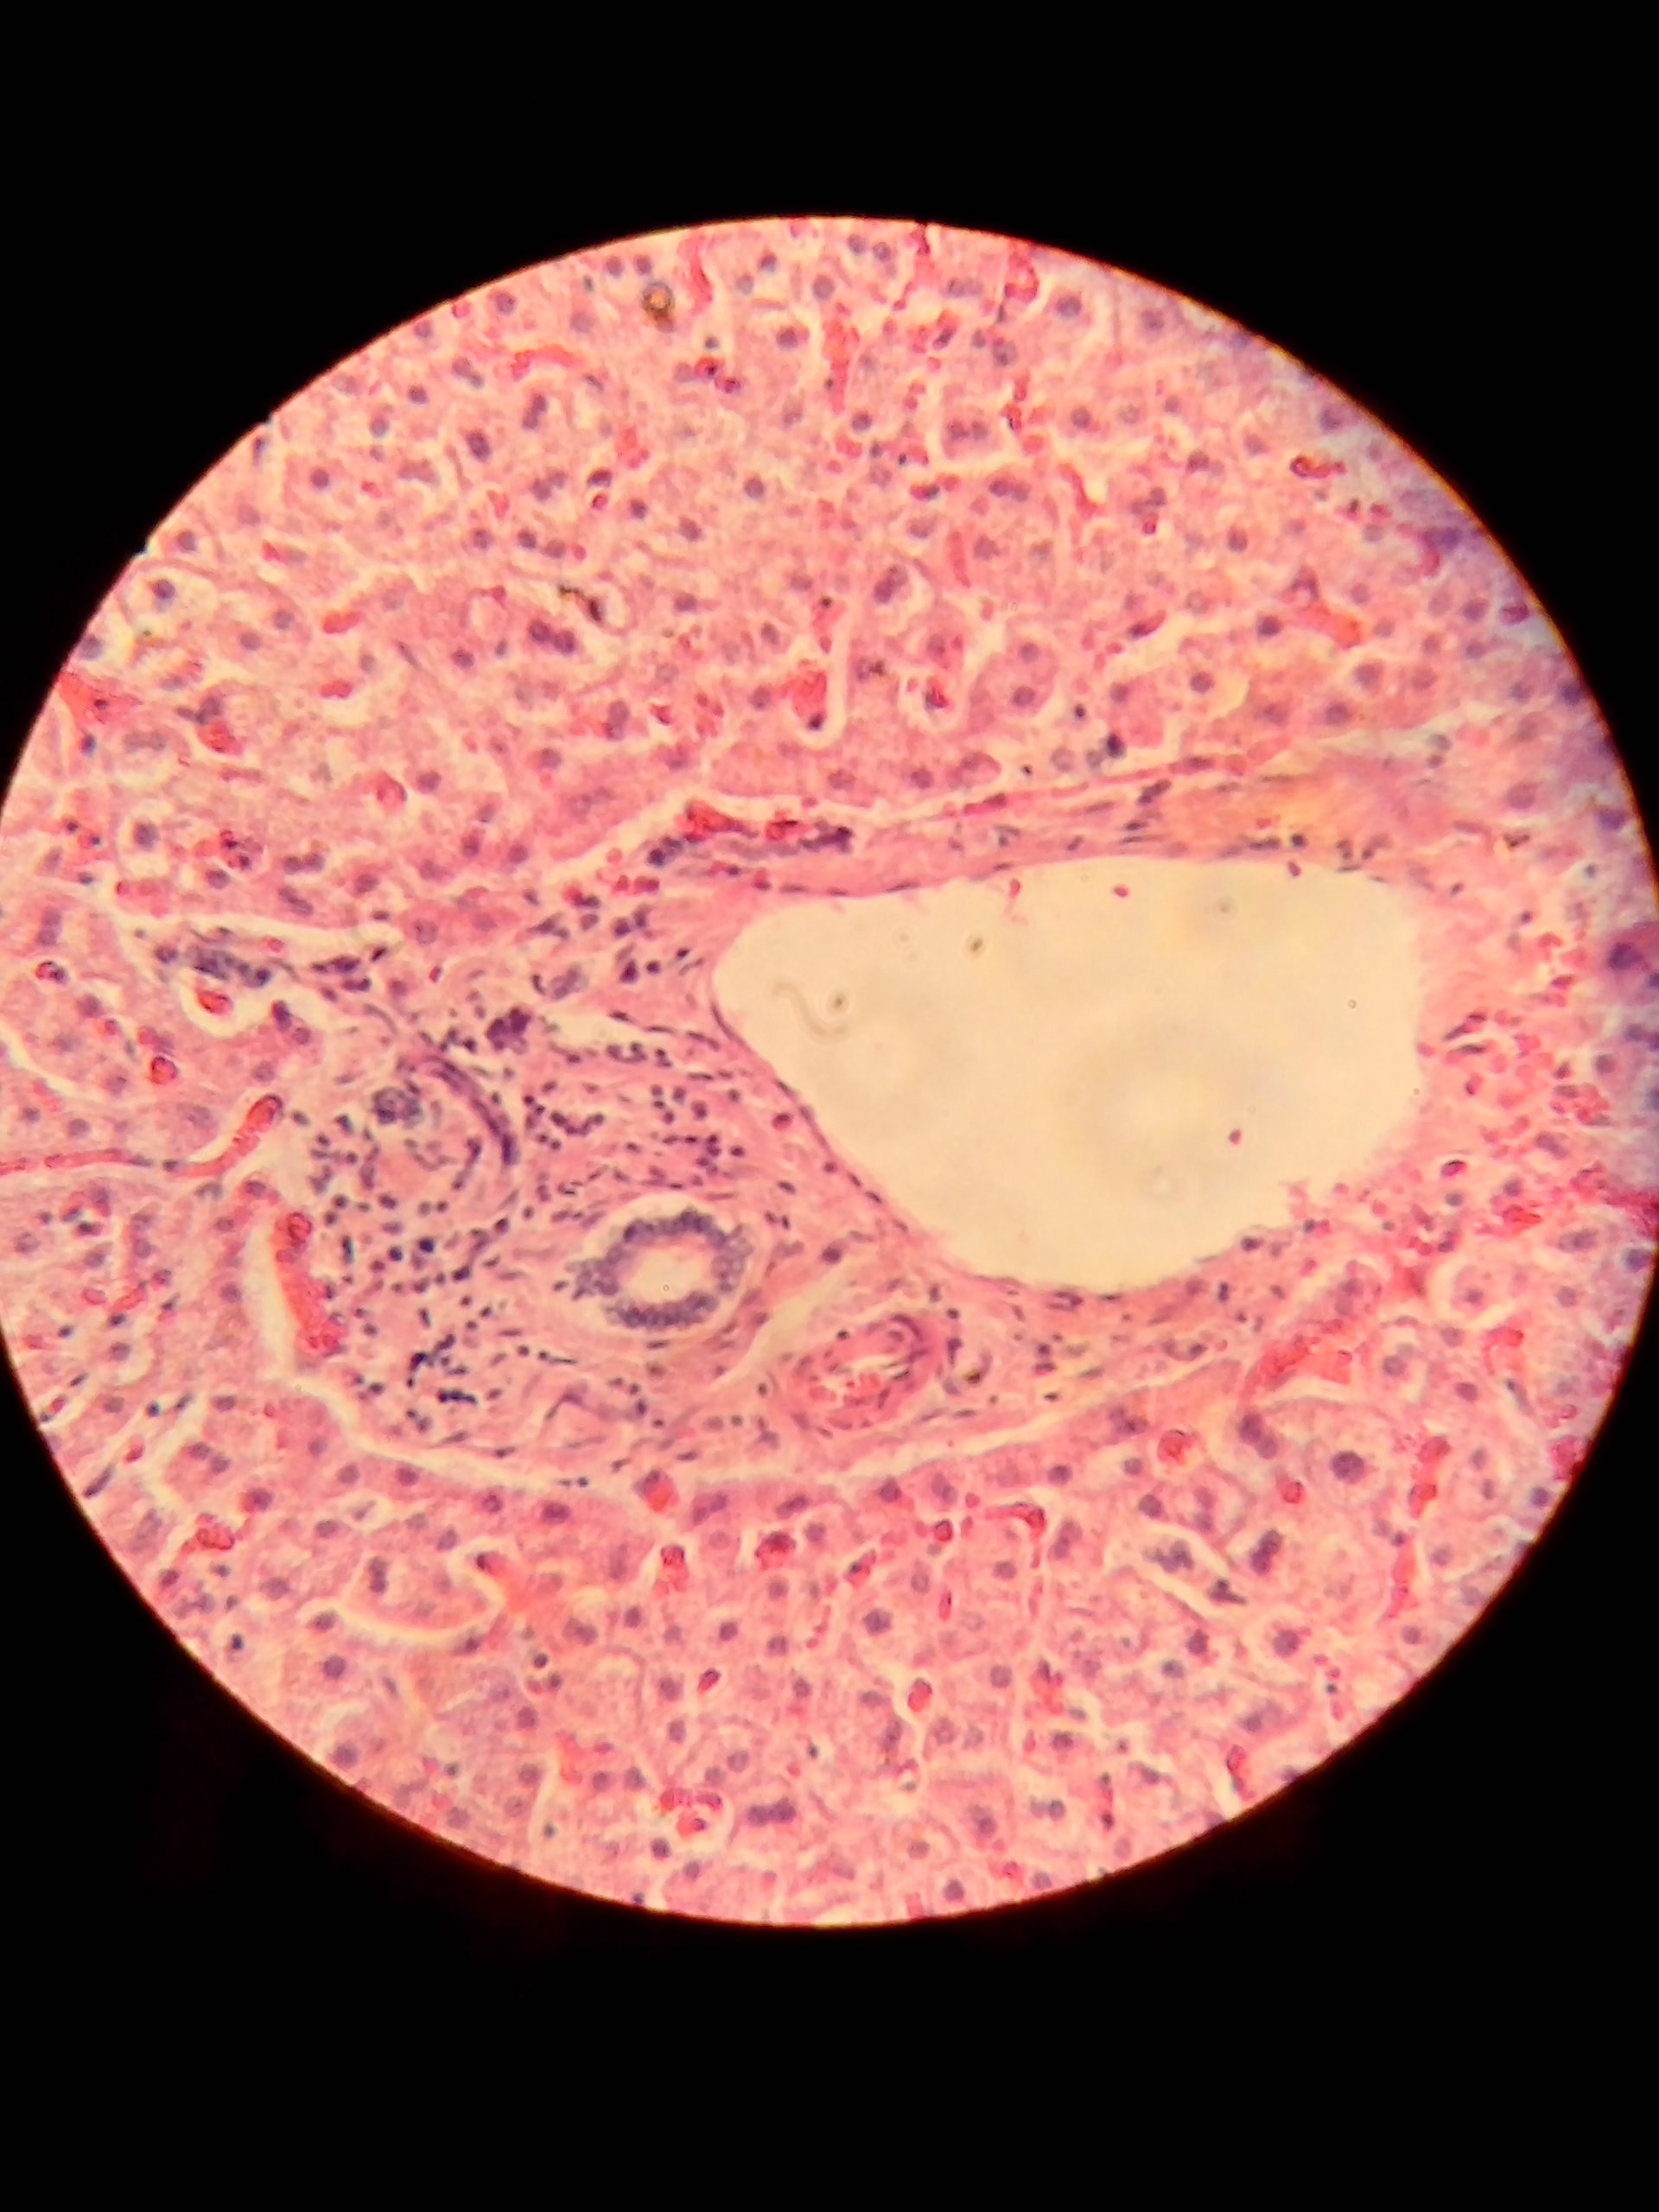
\includegraphics[width=1\textwidth]{../images/07_human_liver.jpg}
		\caption{Vene -- Objektiv 40x}
	\end{subfigure}
	\begin{subfigure}[b]{0.3\textwidth}
		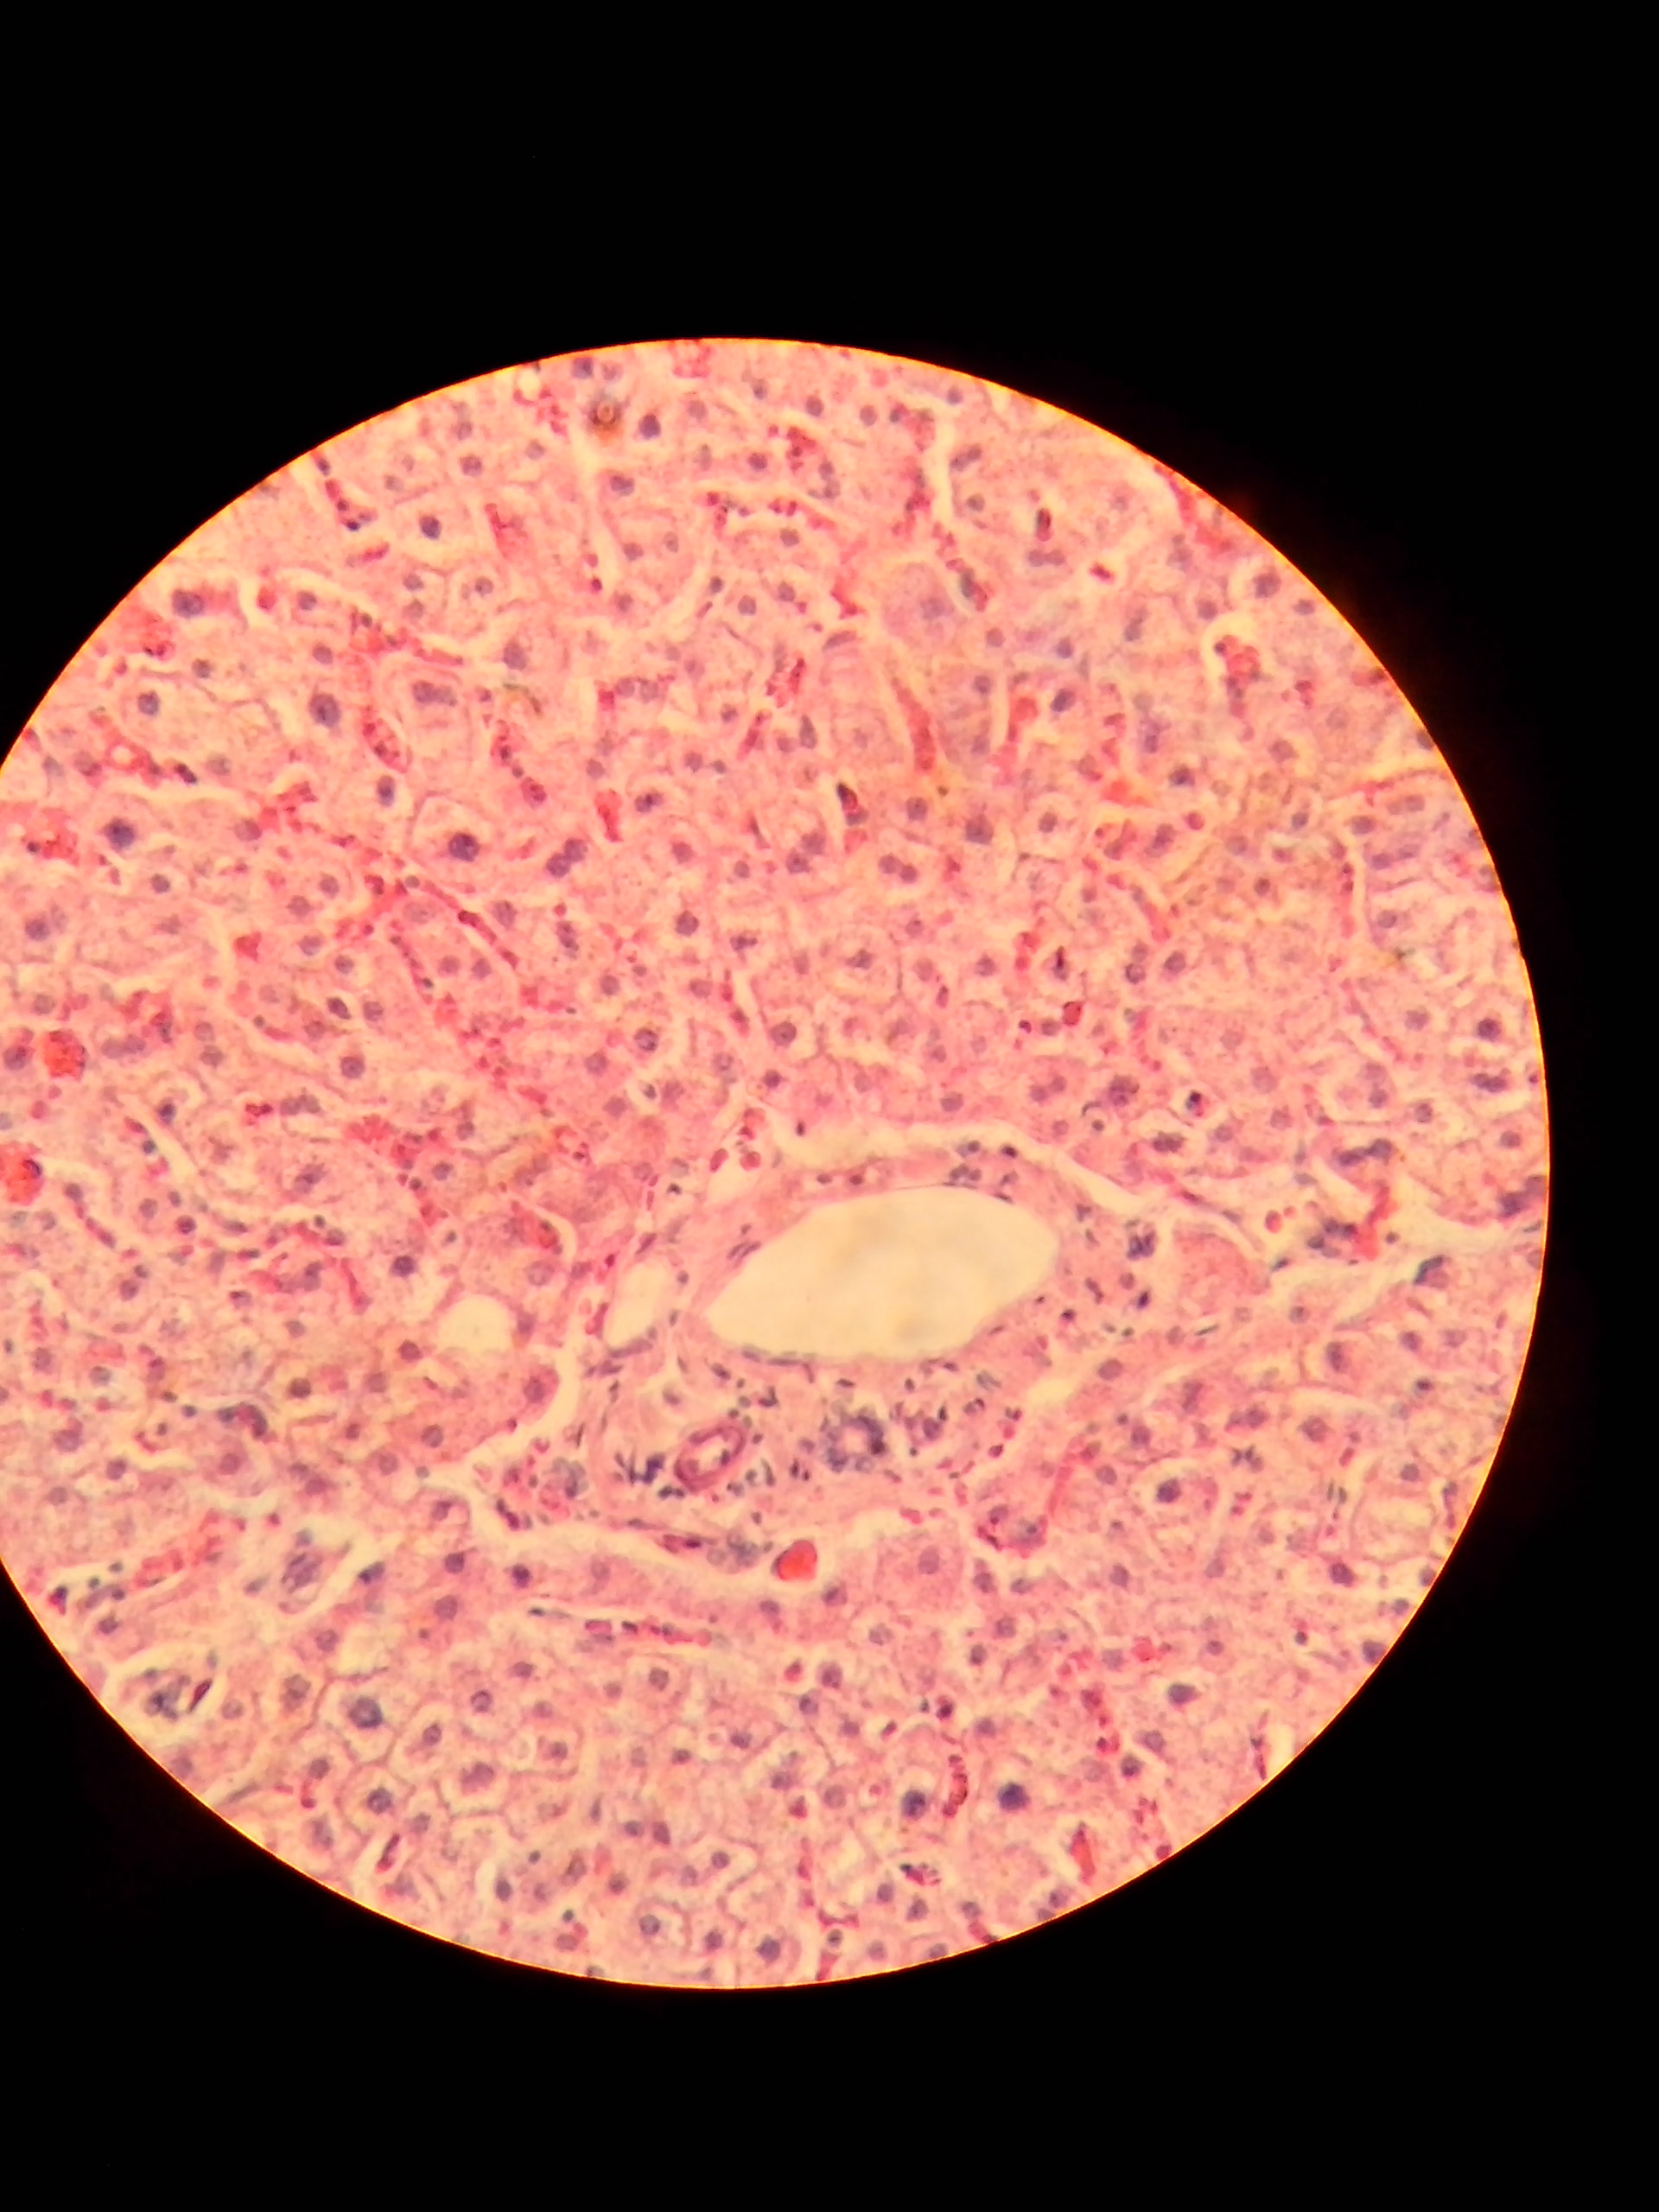
\includegraphics[width=1\textwidth]{../images/08_human_liver.jpg}
		\caption{Galle -- Objektiv 40x}
	\end{subfigure}
	\begin{subfigure}[b]{0.3\textwidth}
		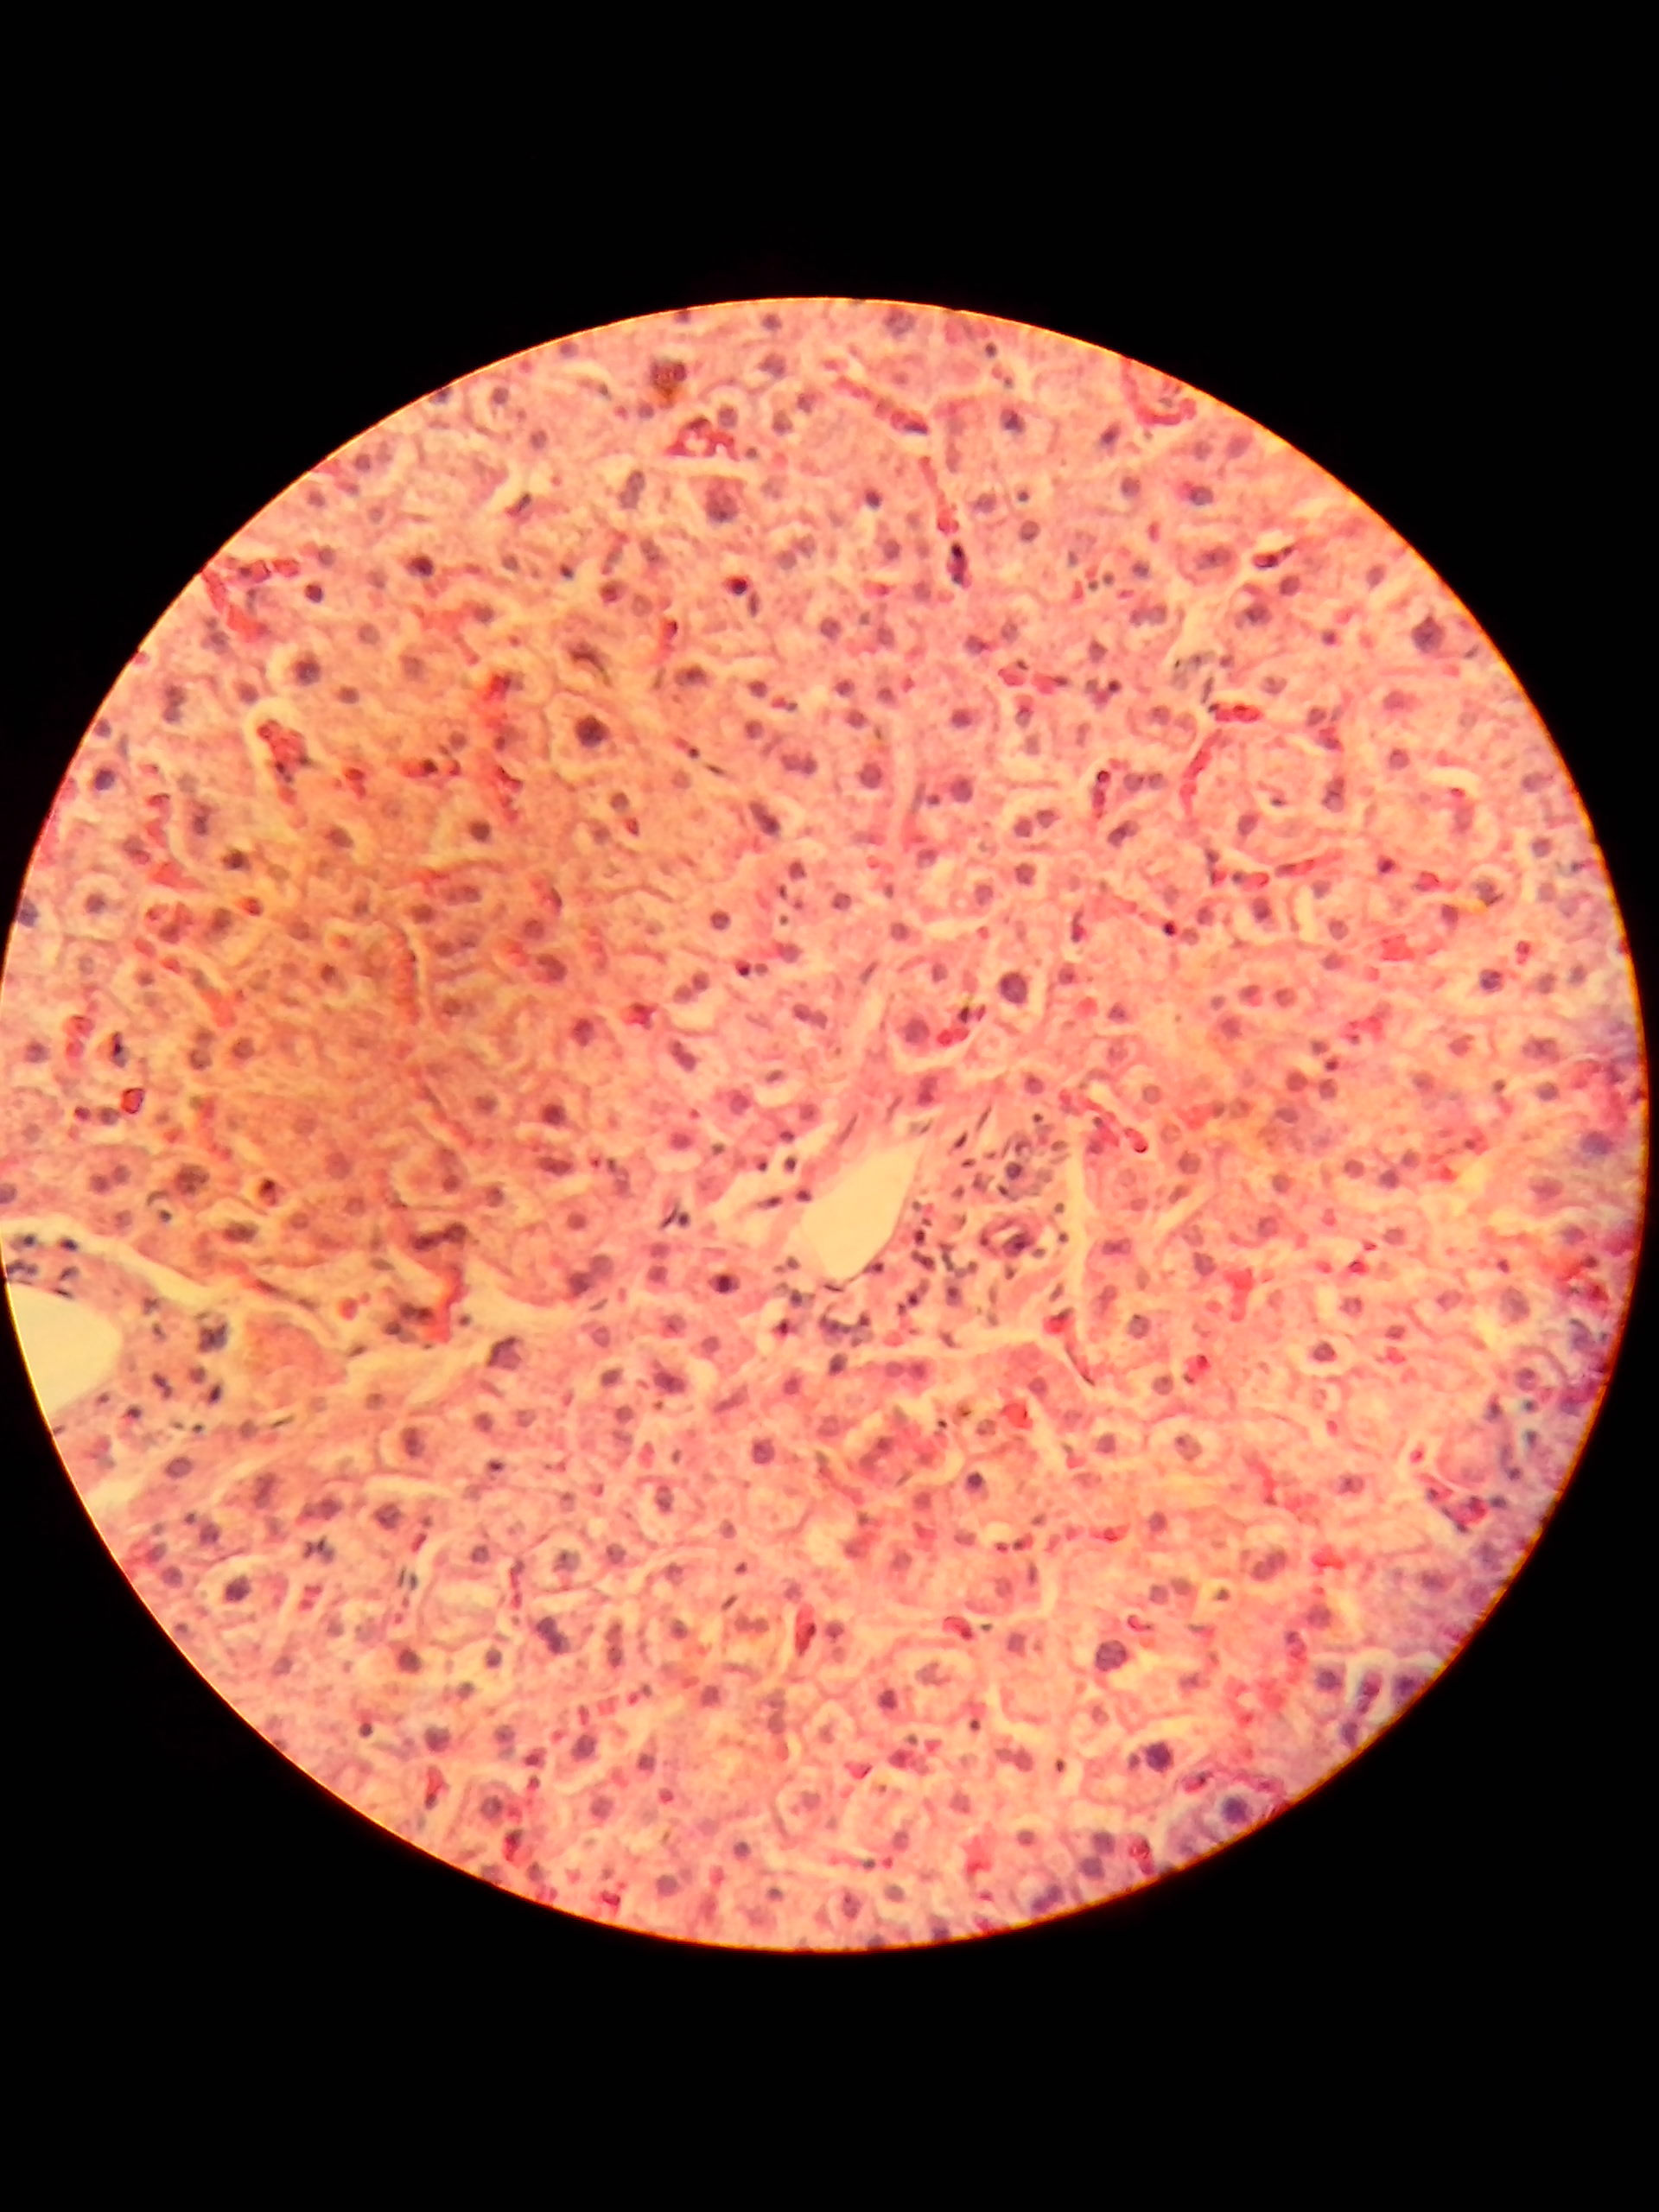
\includegraphics[width=1\textwidth]{../images/10_human_liver.jpg}
		\caption{Arterie -- Objektiv 40x}
	\end{subfigure}
	\caption{Aufzeichnungen der Lichtmikorskopischen Darstellungen der
		menschlichen Leber}
\end{figure}

\subsubsection{Kommentar}


\newpage
\subsection{Menschliche Bauchspeicheldrüse}

\subsubsection{Proben}
\begin{table}[h!]
	\centering
	\begin{tabular}{l l}
		Bezeichnung	& Pankreas \\
		Probe 		& 31-5442
	\end{tabular}
\end{table}

\subsubsection{Aufzeichnungen}
\begin{figure}[h!]
	\centering
	\begin{subfigure}[b]{0.3\textwidth}
		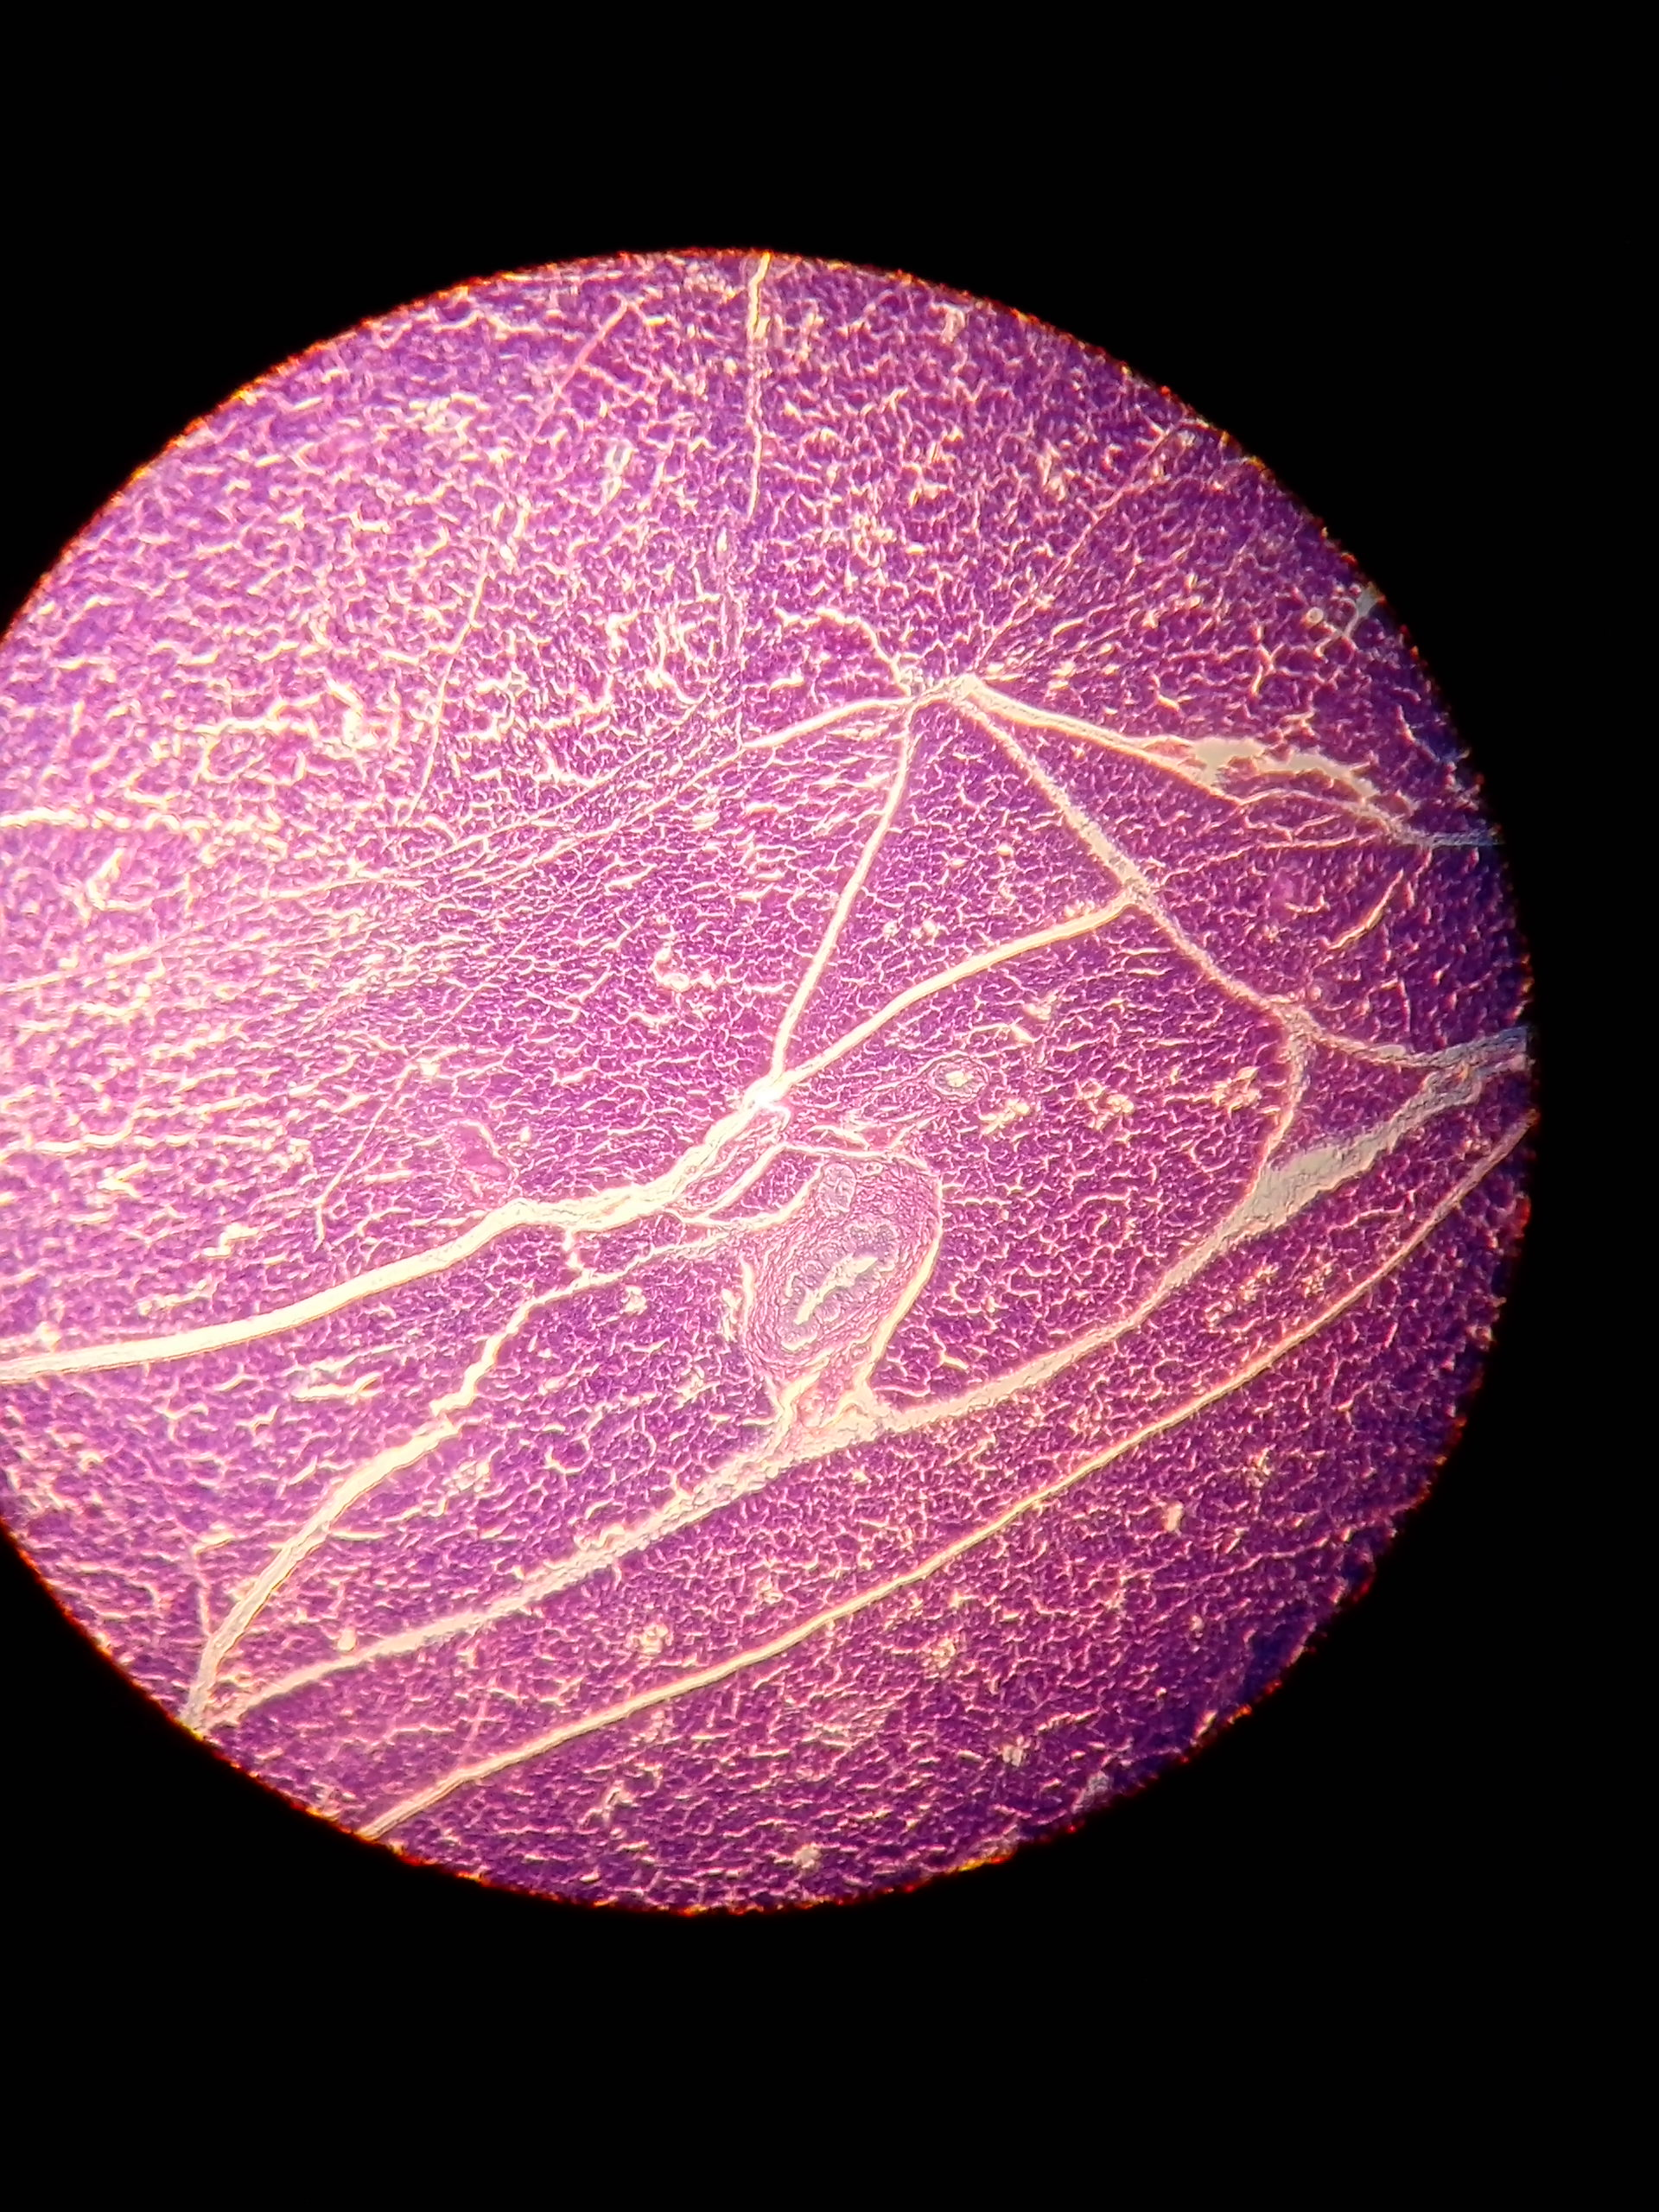
\includegraphics[width=1\textwidth]{../images/01_pankreas.jpg}
		\caption{Objektiv 10x}
	\end{subfigure}
	\begin{subfigure}[b]{0.3\textwidth}
		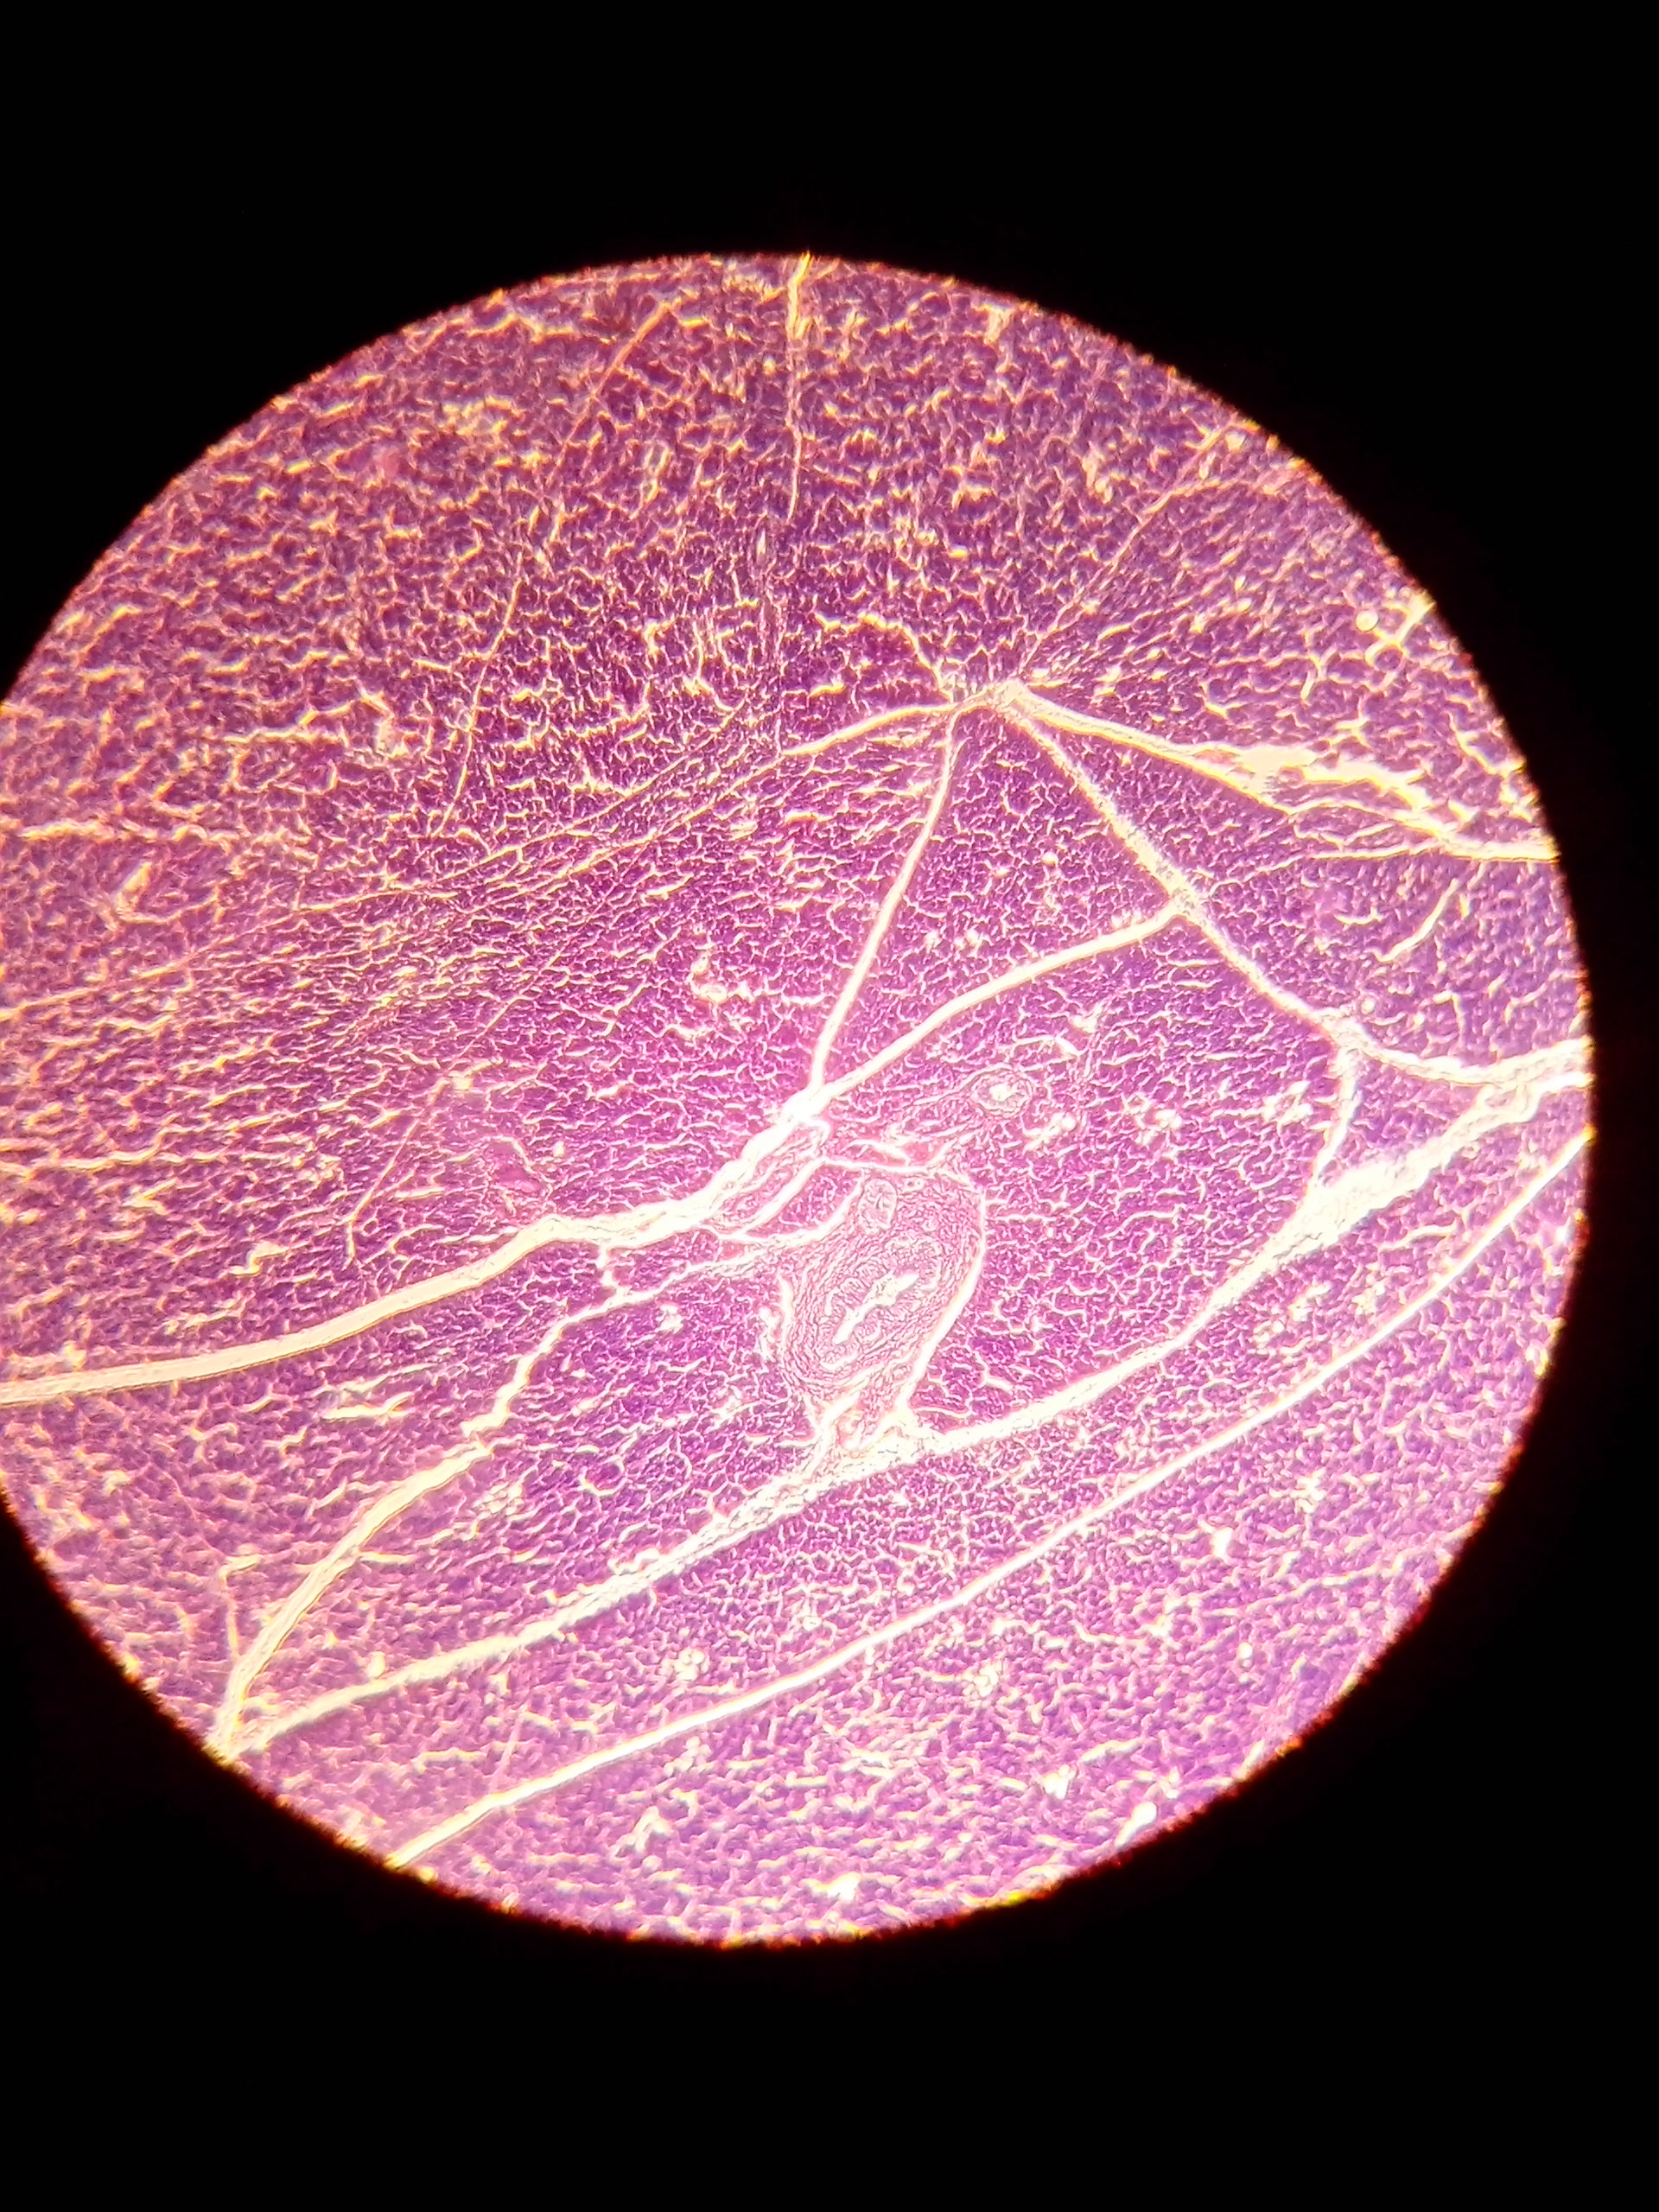
\includegraphics[width=1\textwidth]{../images/02_pankreas.jpg}
		\caption{Objektiv 10x}
	\end{subfigure}

	\begin{subfigure}[b]{0.3\textwidth}
		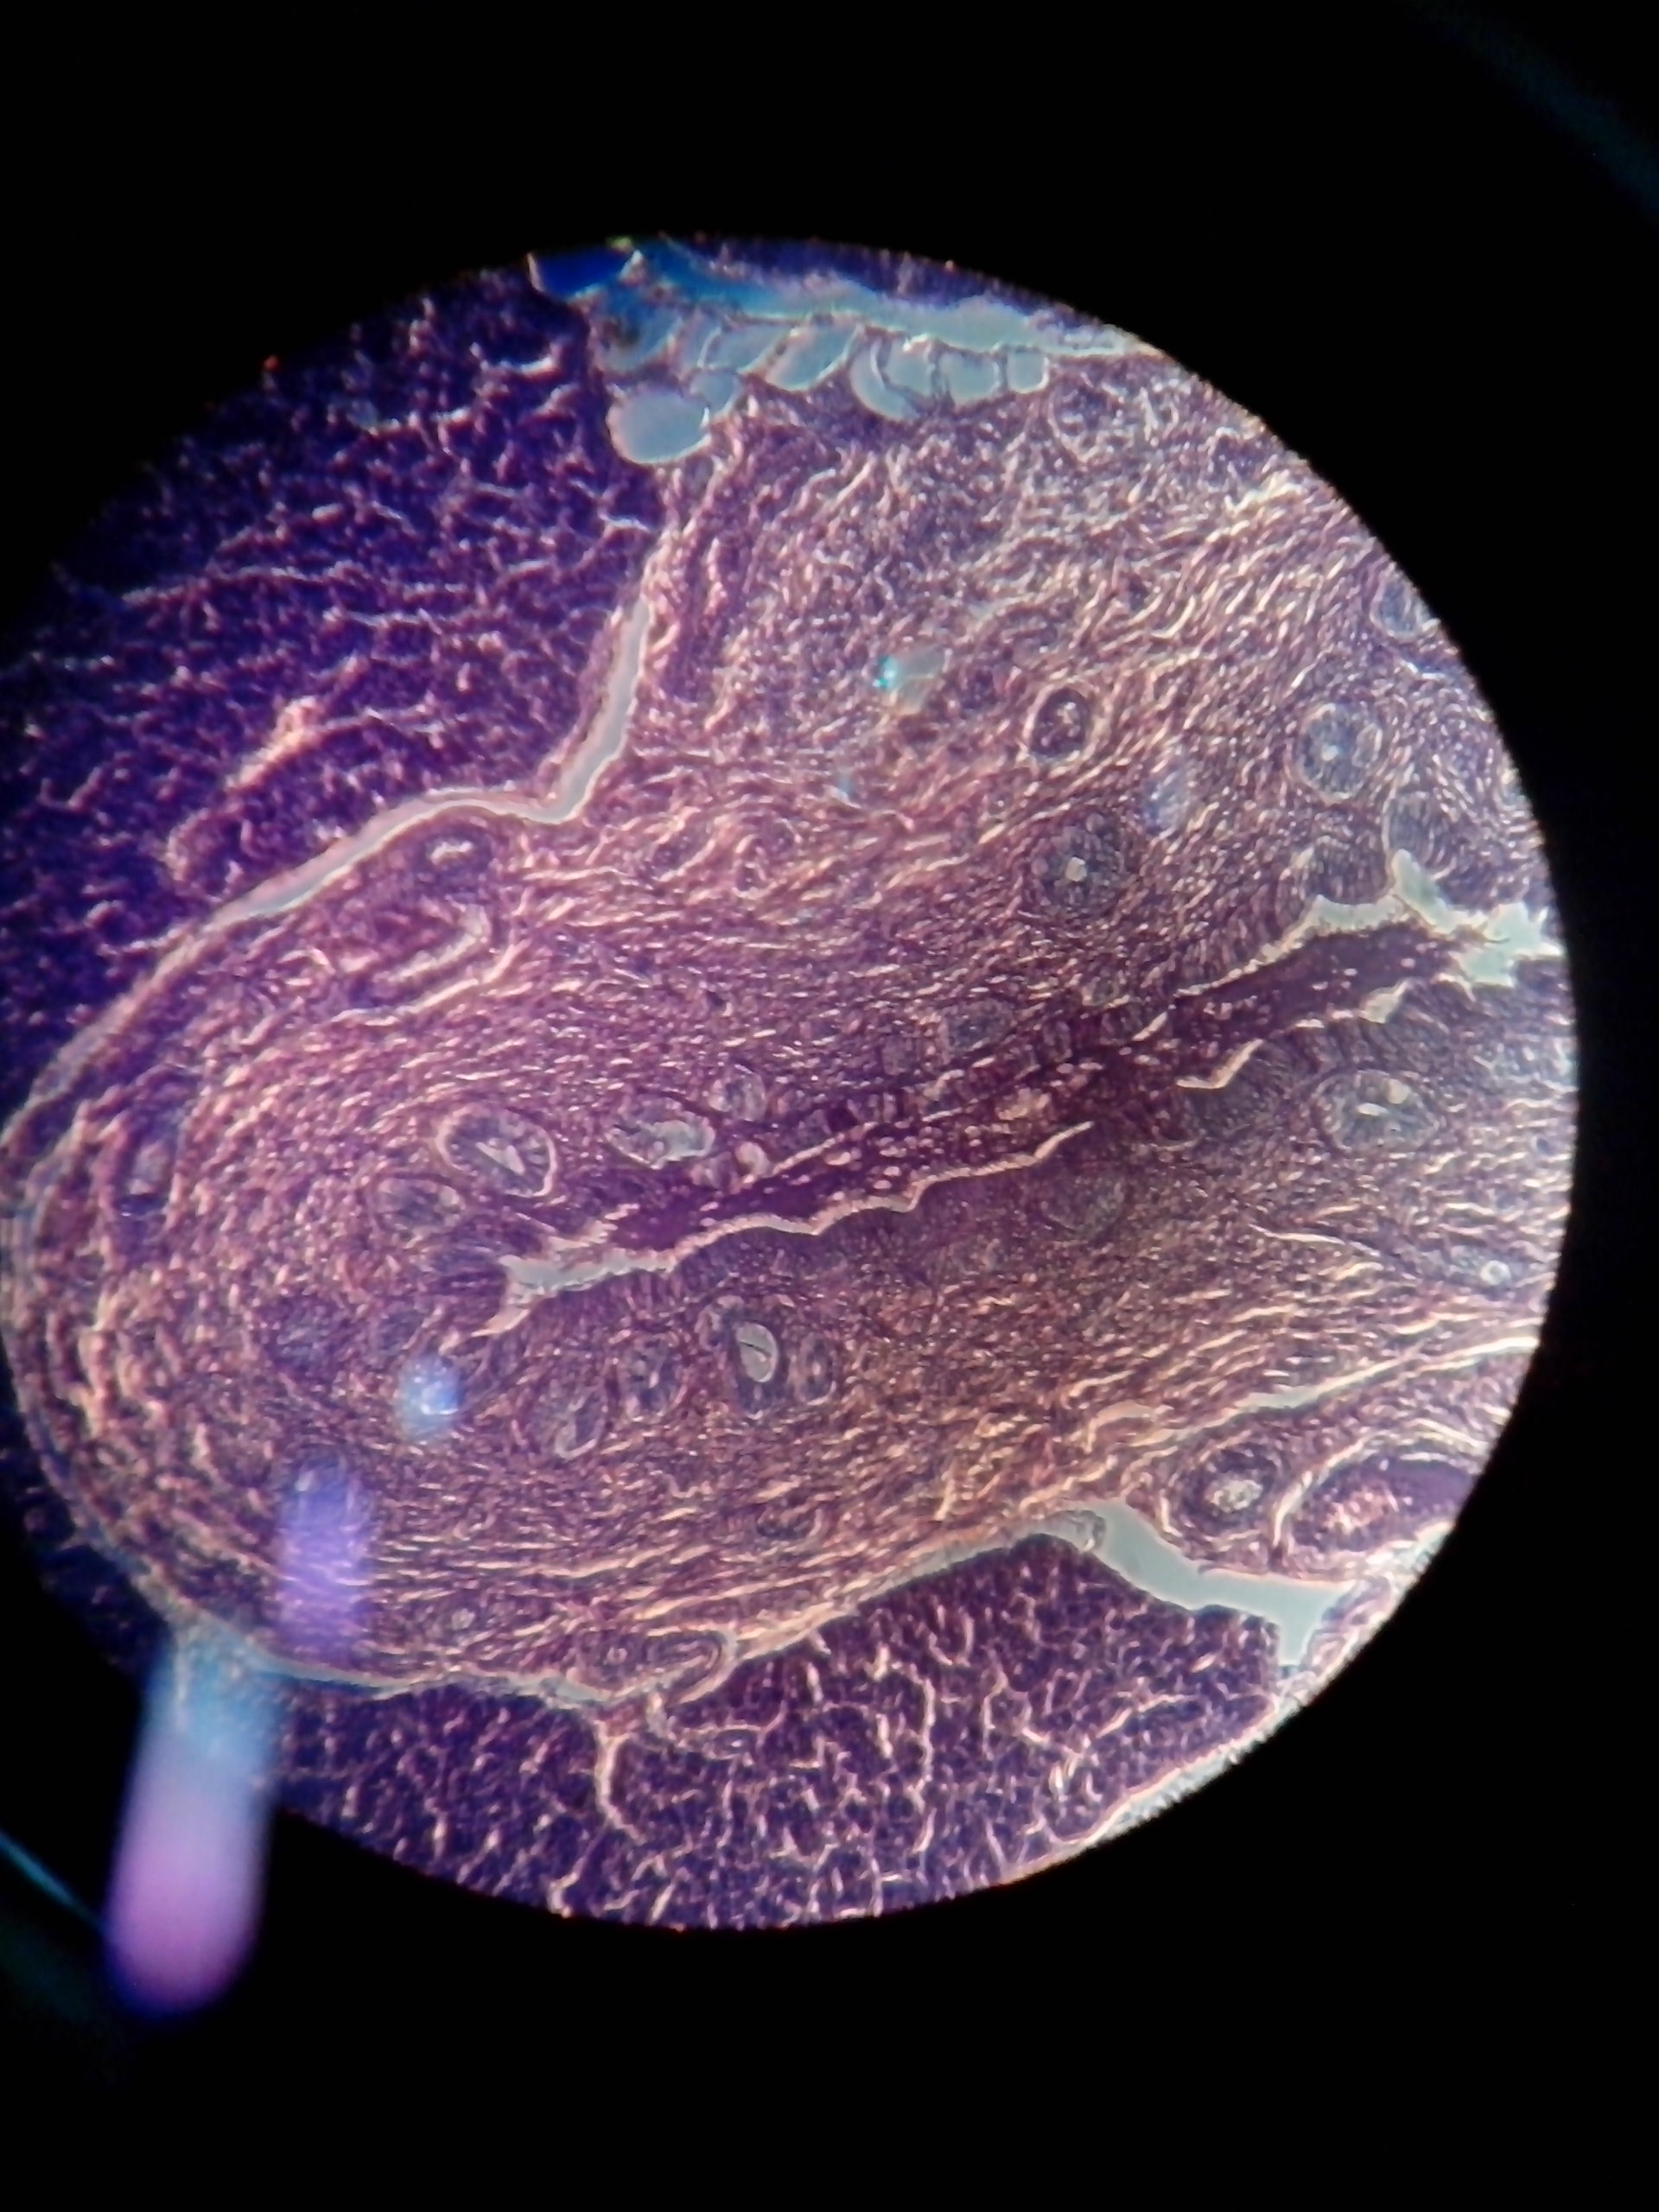
\includegraphics[width=1\textwidth]{../images/03_pankreas.jpg}
		\caption{Objektiv 20x}
	\end{subfigure}
	\begin{subfigure}[b]{0.3\textwidth}
		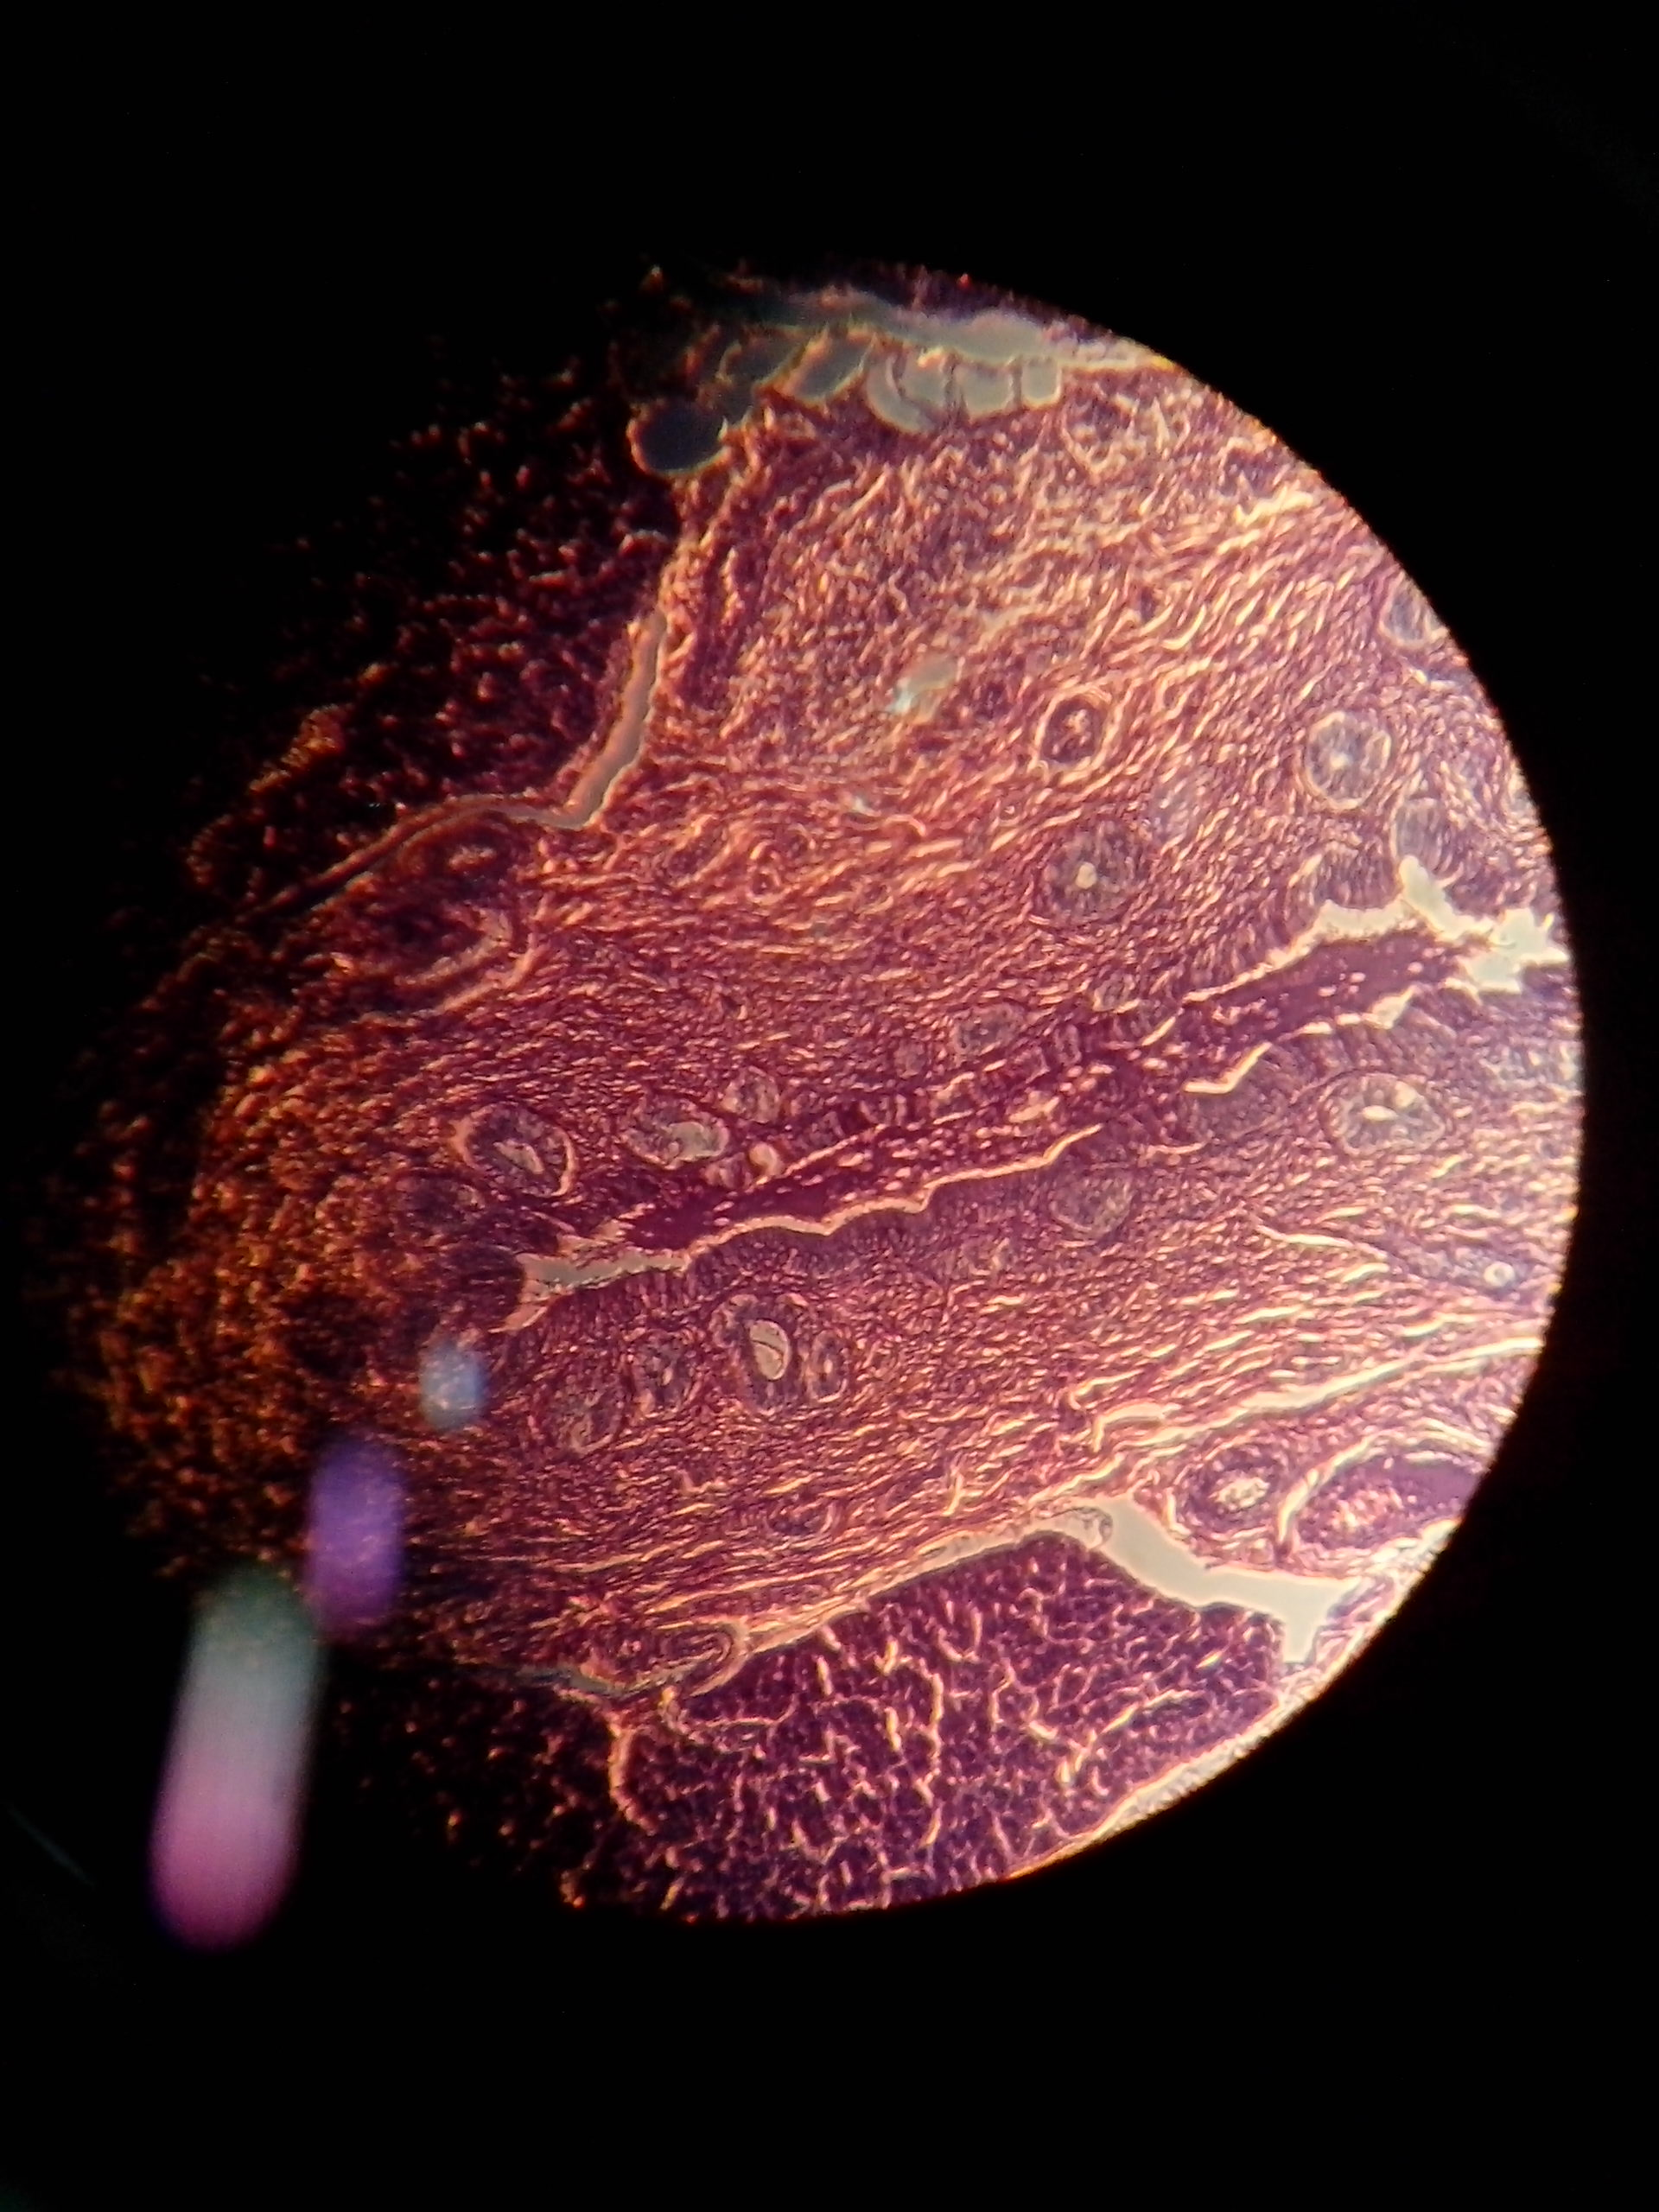
\includegraphics[width=1\textwidth]{../images/04_pankreas.jpg}
		\caption{Objektiv 20x}
	\end{subfigure}
	\caption{Aufzeichnungen der Lichtmikorskopischen Darstellungen der
		menschlichen Bauchspeicheldrüse}
\end{figure}

\subsubsection{Kommentar}

\newpage
\subsection{Menschlicher Magen}

\subsubsection{Proben}
\begin{table}[h!]
	\centering
	\begin{tabular}{l l}
		Bezeichnung	& human stomach \\
		Probe 		& 31-5100
	\end{tabular}
\end{table}

\subsubsection{Aufzeichnungen}
\begin{figure}[h!]
	\centering
	\begin{subfigure}[b]{0.3\textwidth}
		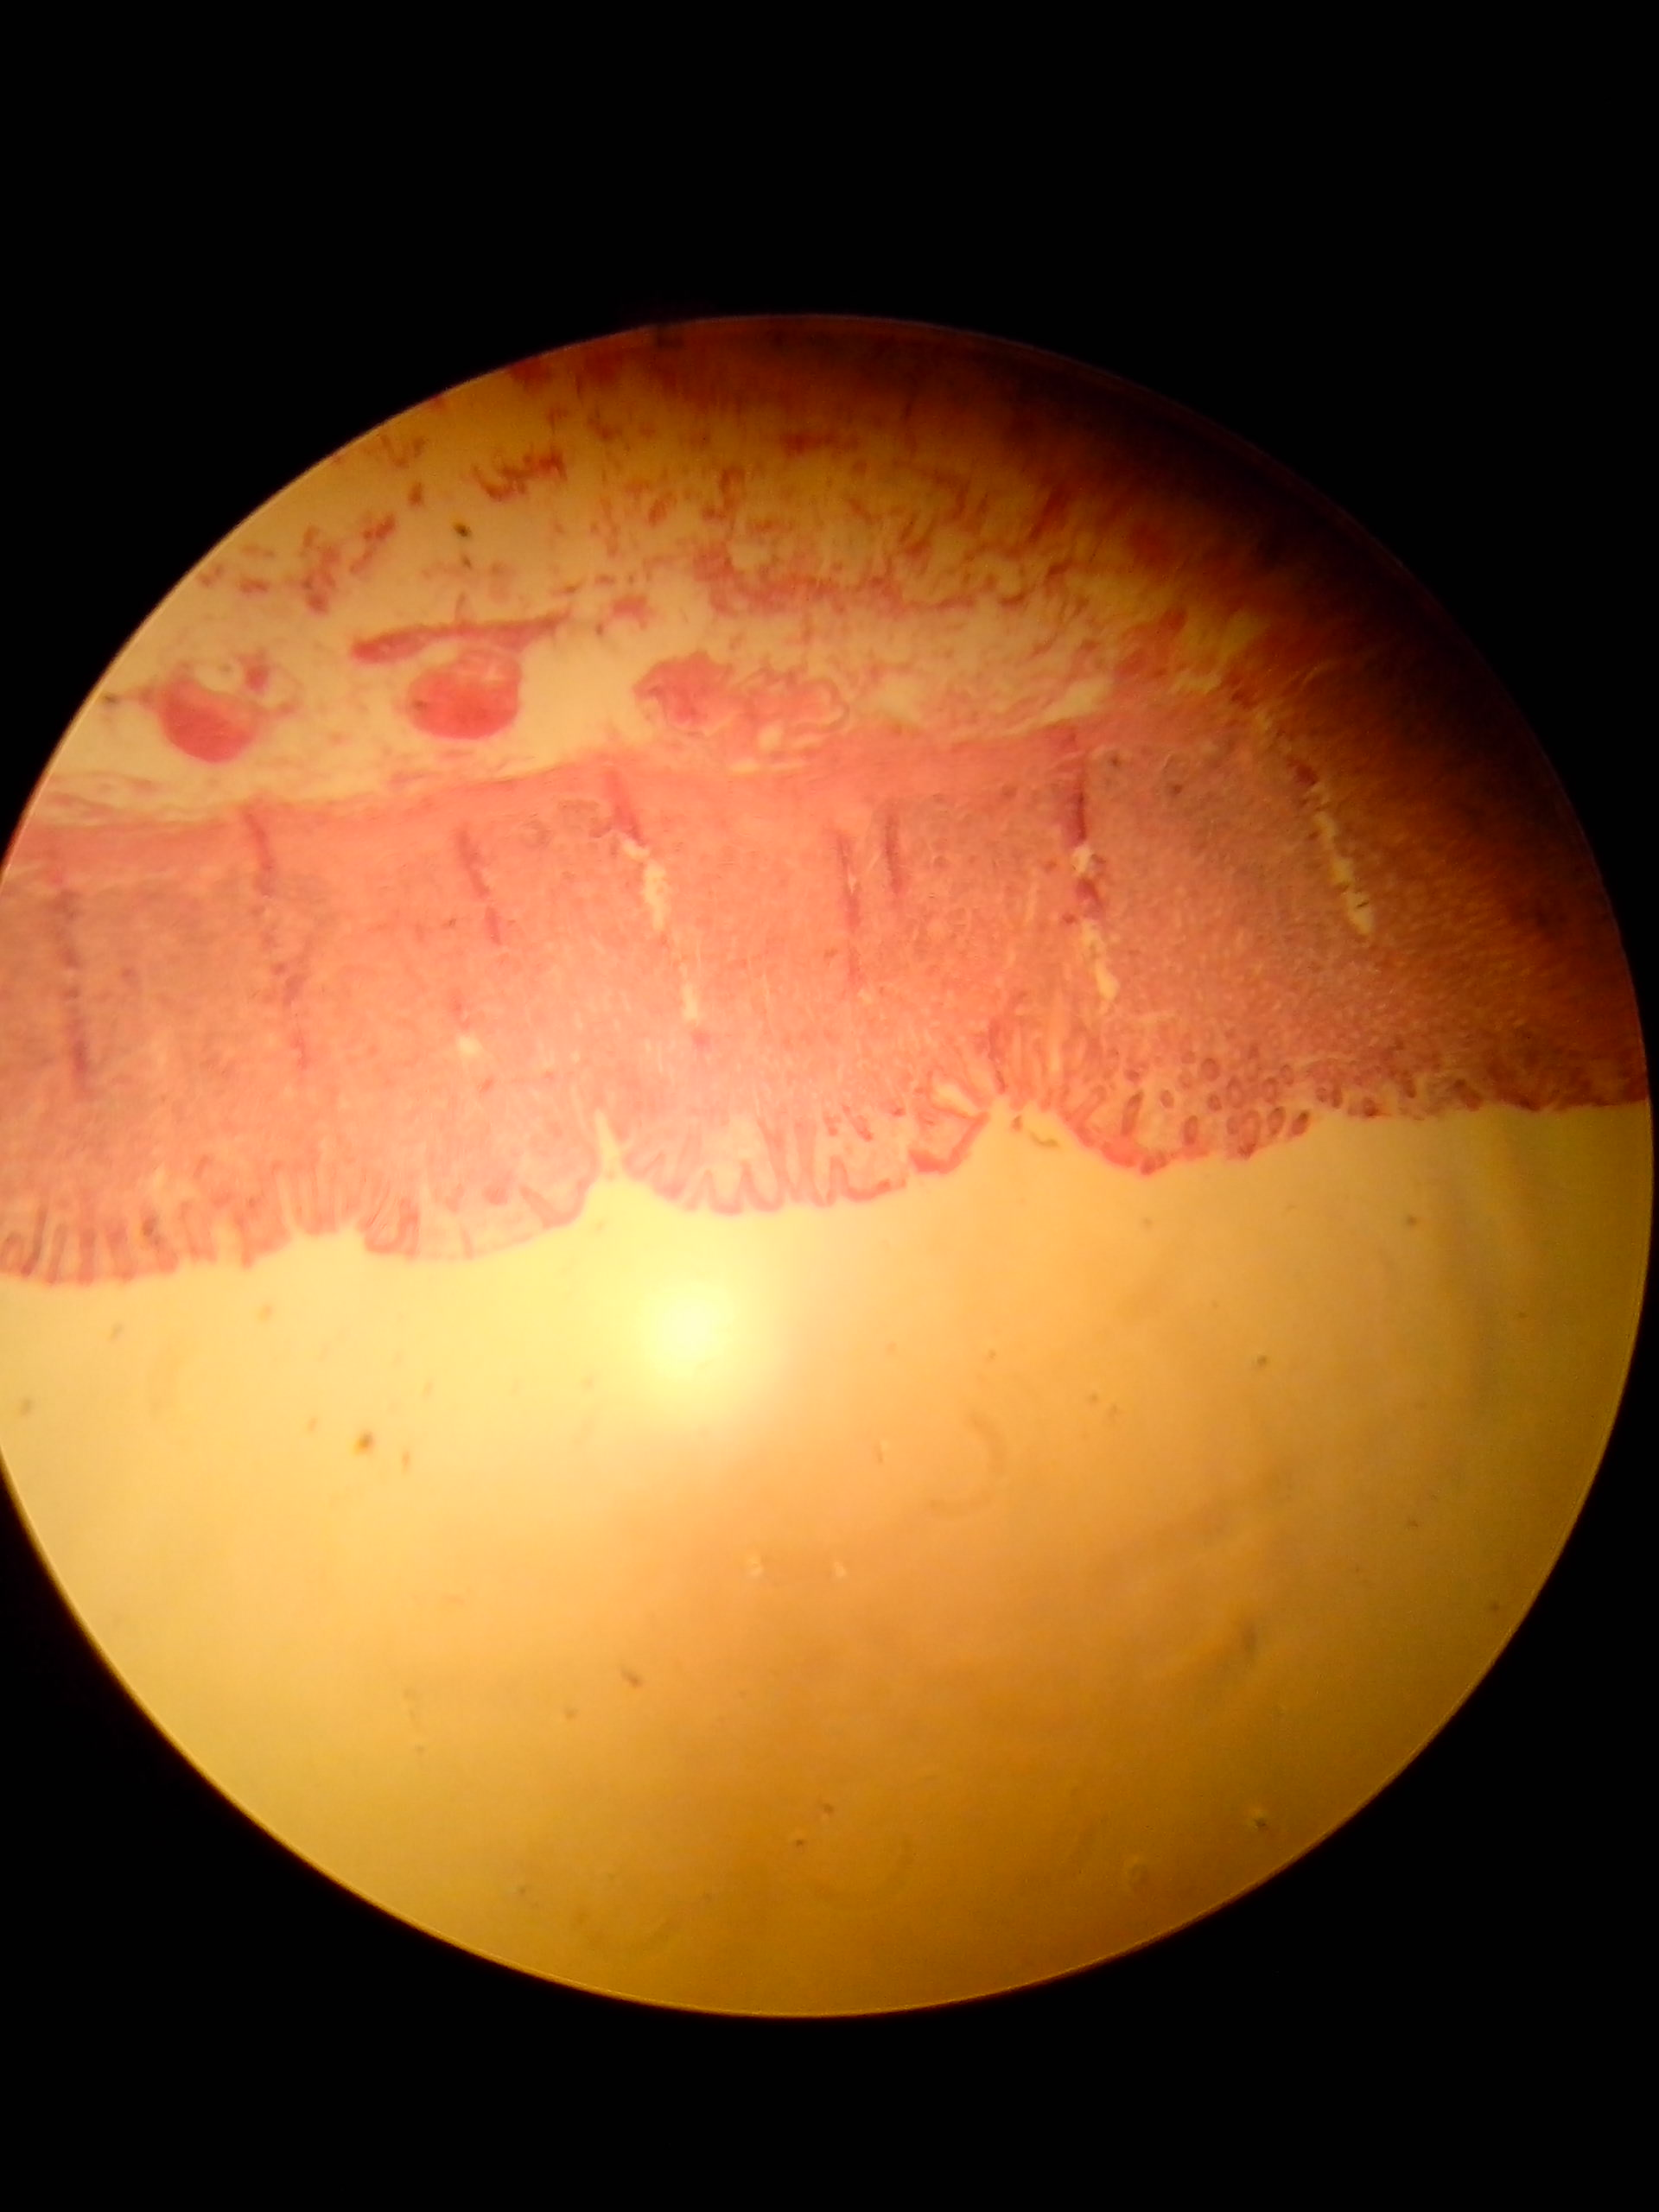
\includegraphics[width=1\textwidth]{../images/01_stomach.jpg}
		\caption{Objektiv 4x}
	\end{subfigure}
	\begin{subfigure}[b]{0.3\textwidth}
		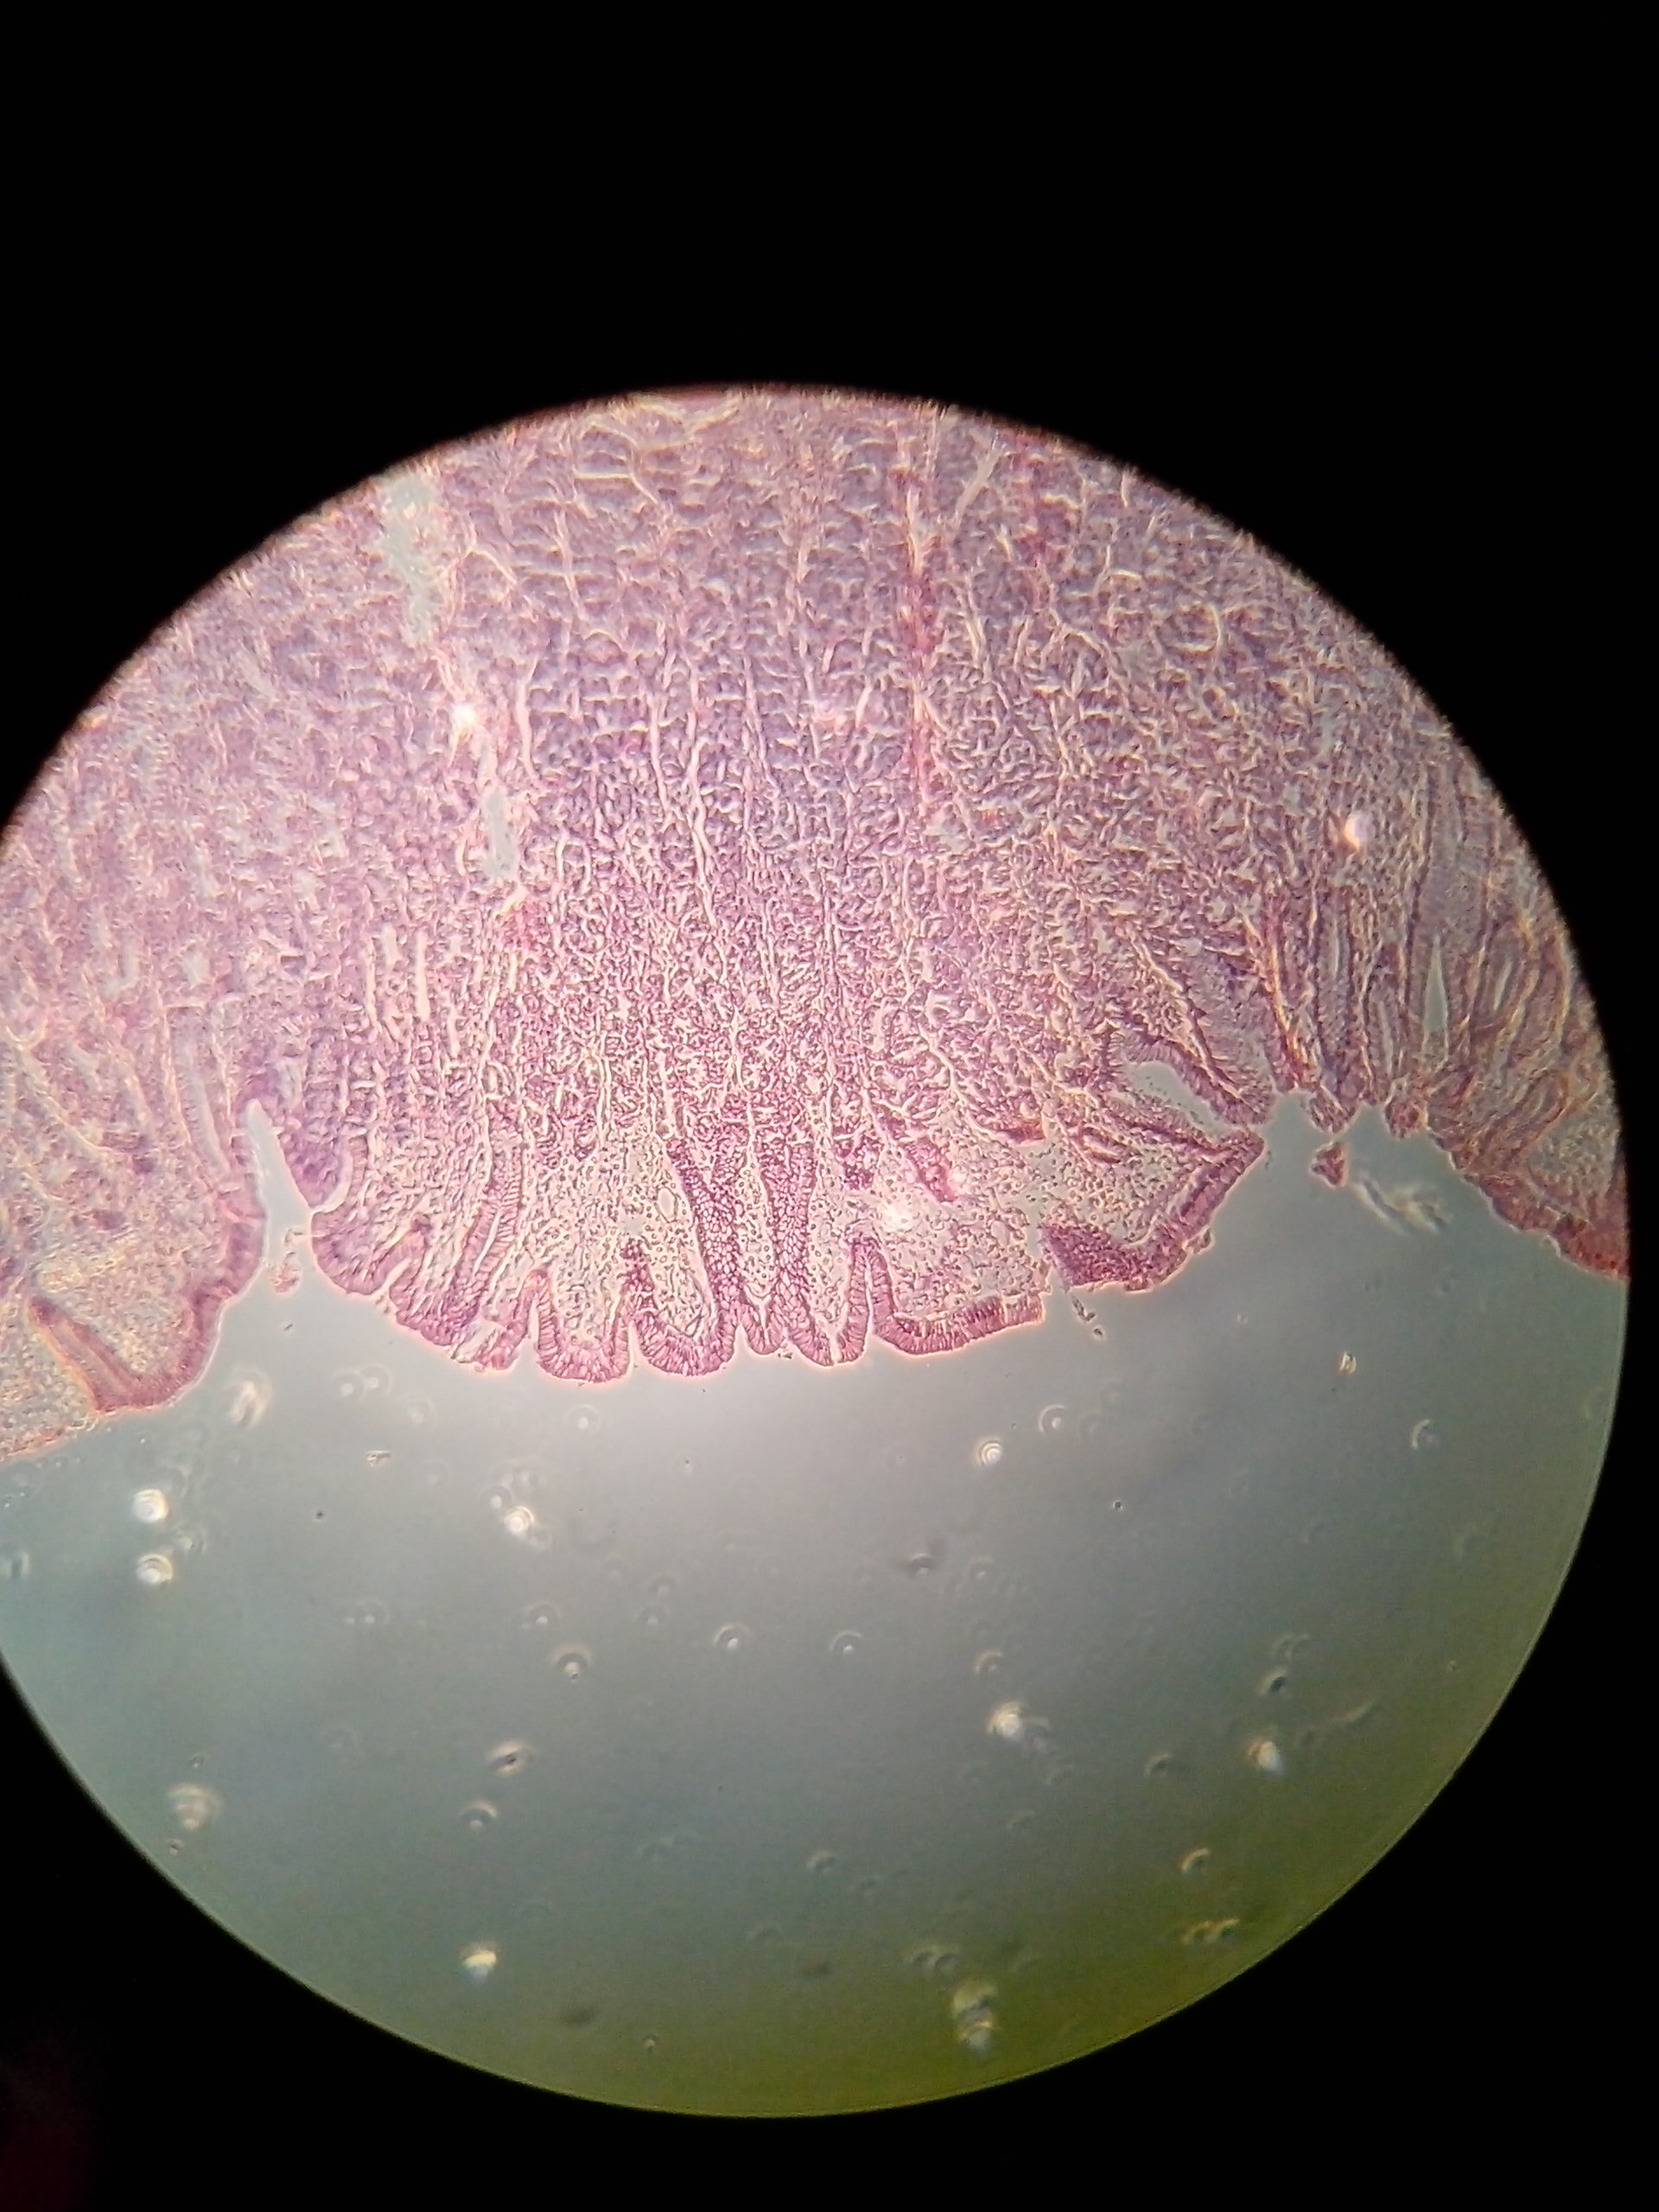
\includegraphics[width=1\textwidth]{../images/02_stomach.jpg}
		\caption{Objektiv 10x}
	\end{subfigure}
	\begin{subfigure}[b]{0.3\textwidth}
		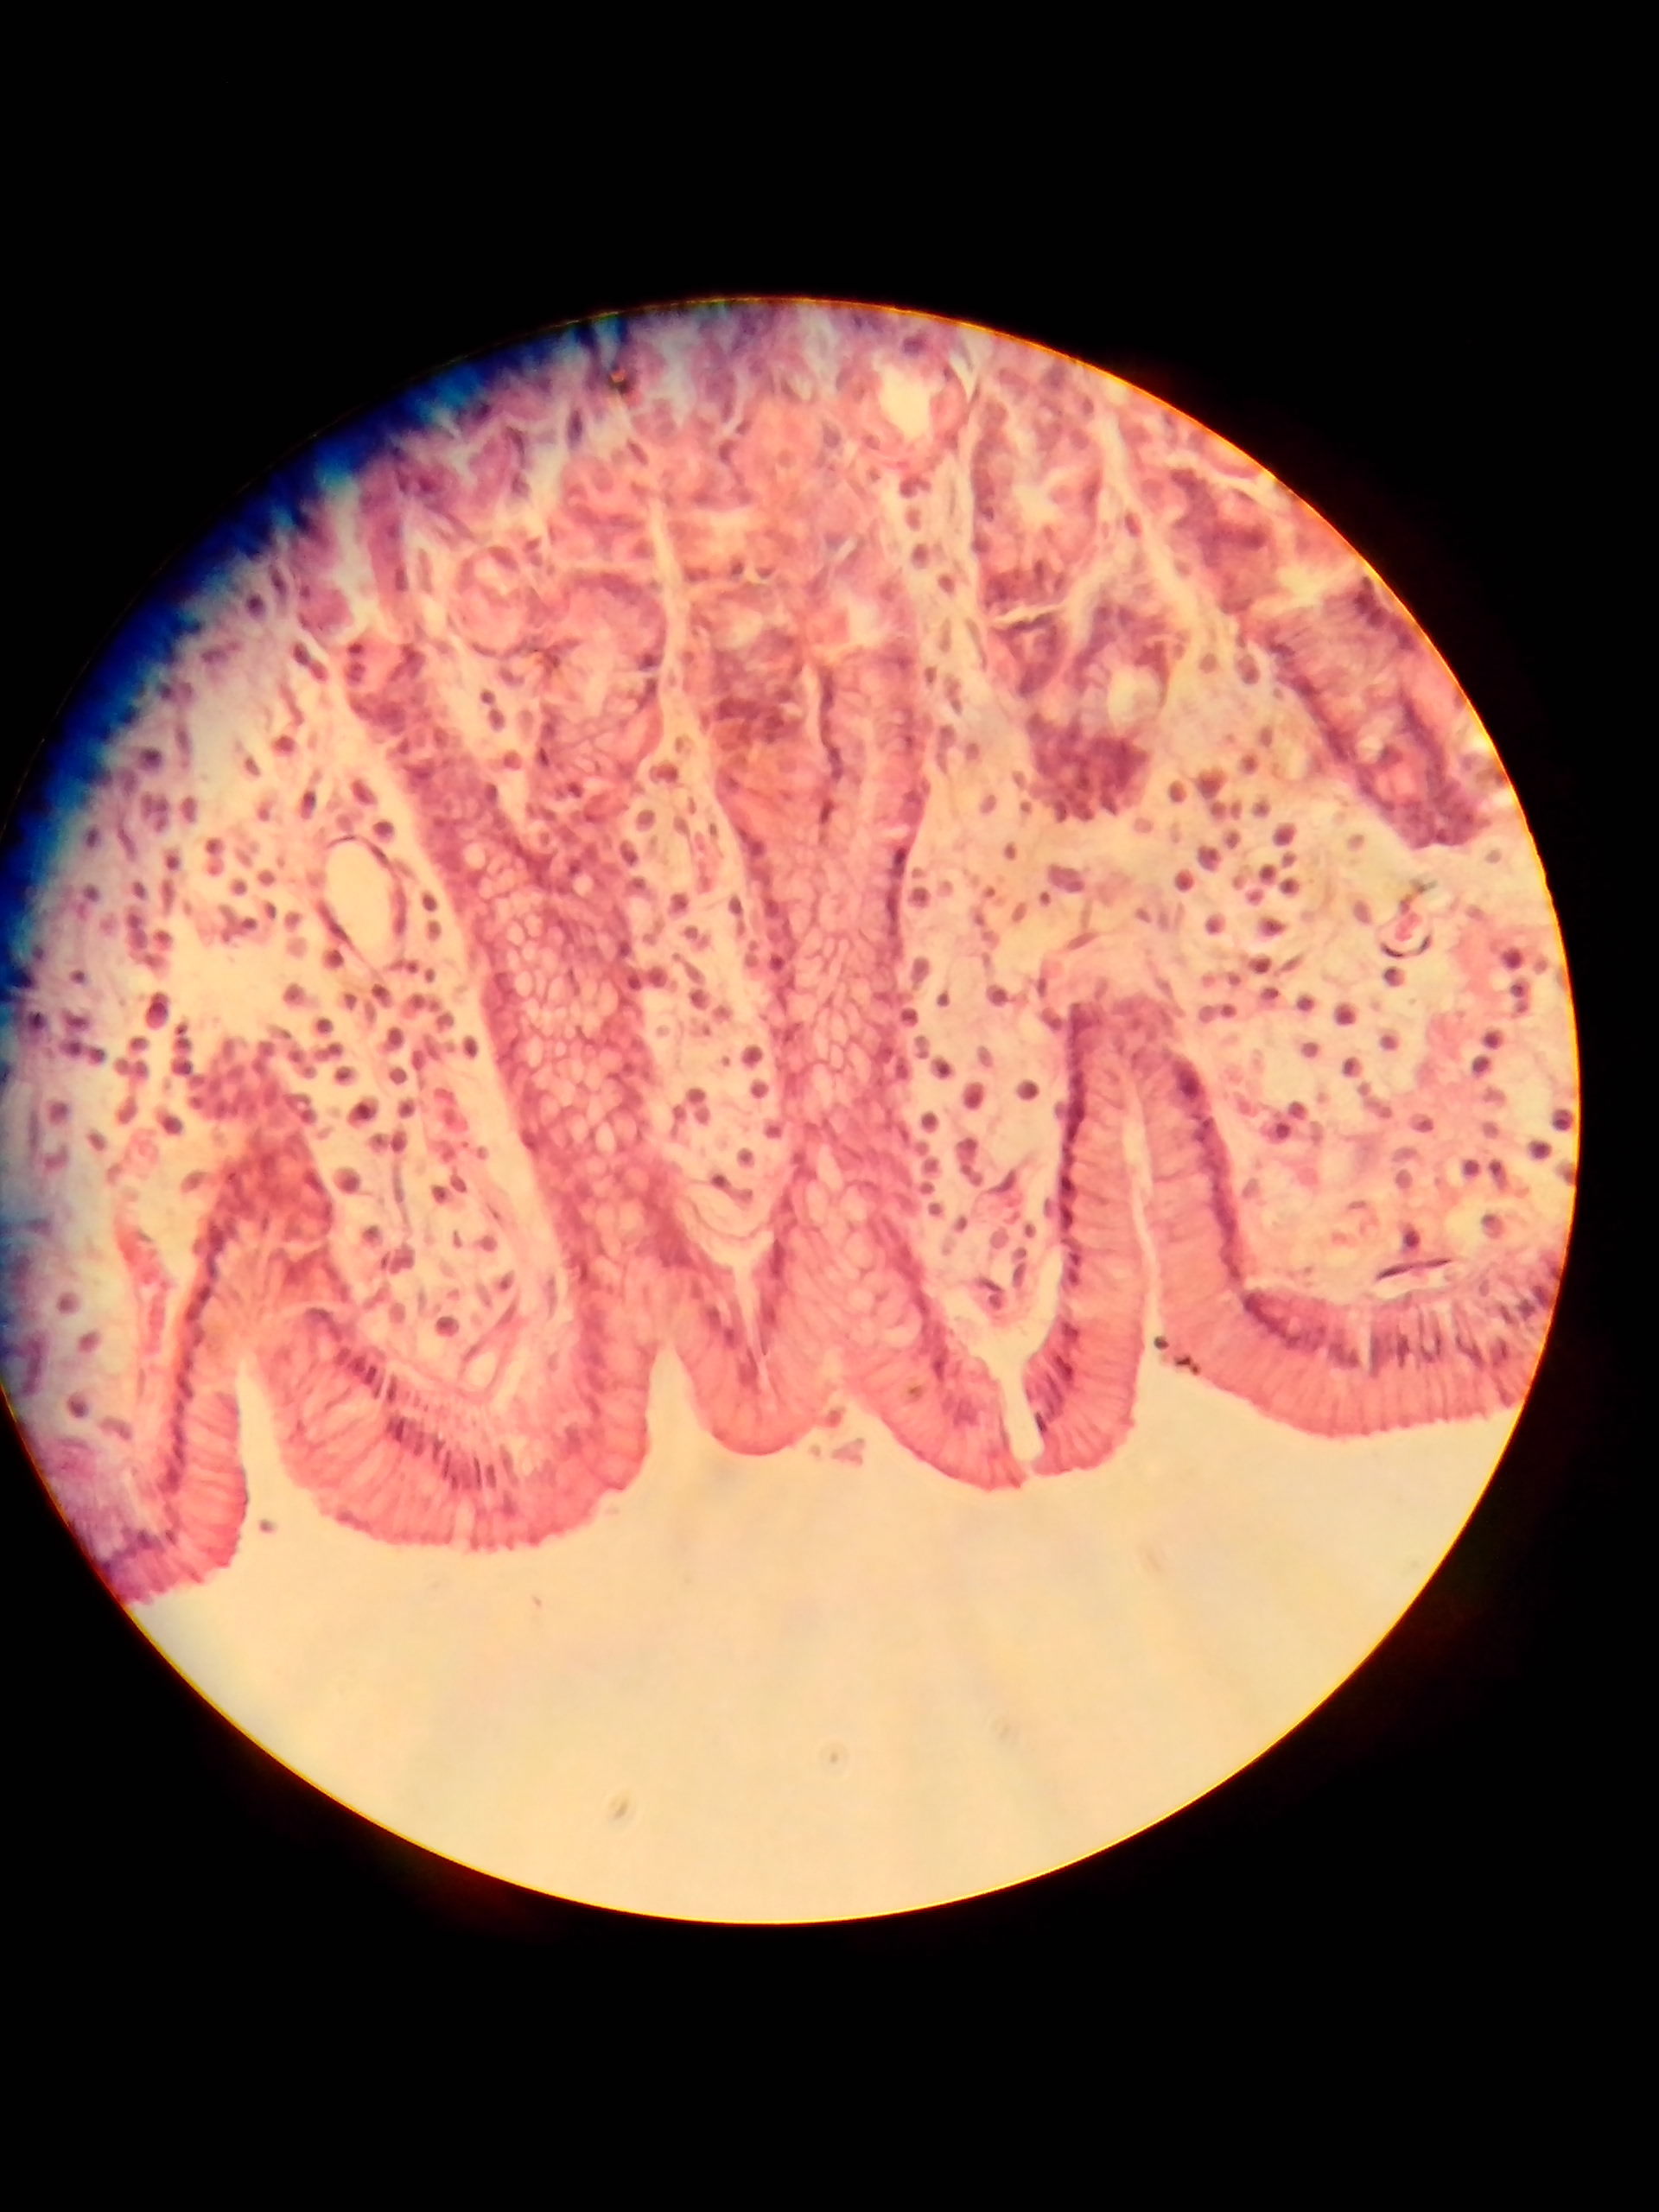
\includegraphics[width=1\textwidth]{../images/03_stomach.jpg}
		\caption{Objektiv 20x}
	\end{subfigure}
	\caption{Aufzeichnungen der Lichtmikorskopischen Darstellungen de
		menschlichen Magens}
\end{figure}

\subsubsection{Kommentar}

\newpage
\subsection{Menschliche Aorta}

\subsubsection{Proben}
\begin{table}[h!]
	\centering
	\begin{tabular}{l l}
		Bezeichnung	& human aorta \\
		Probe 		& n.a.
	\end{tabular}
\end{table}

\subsubsection{Aufzeichnungen}
\begin{figure}[h!]
	\centering
		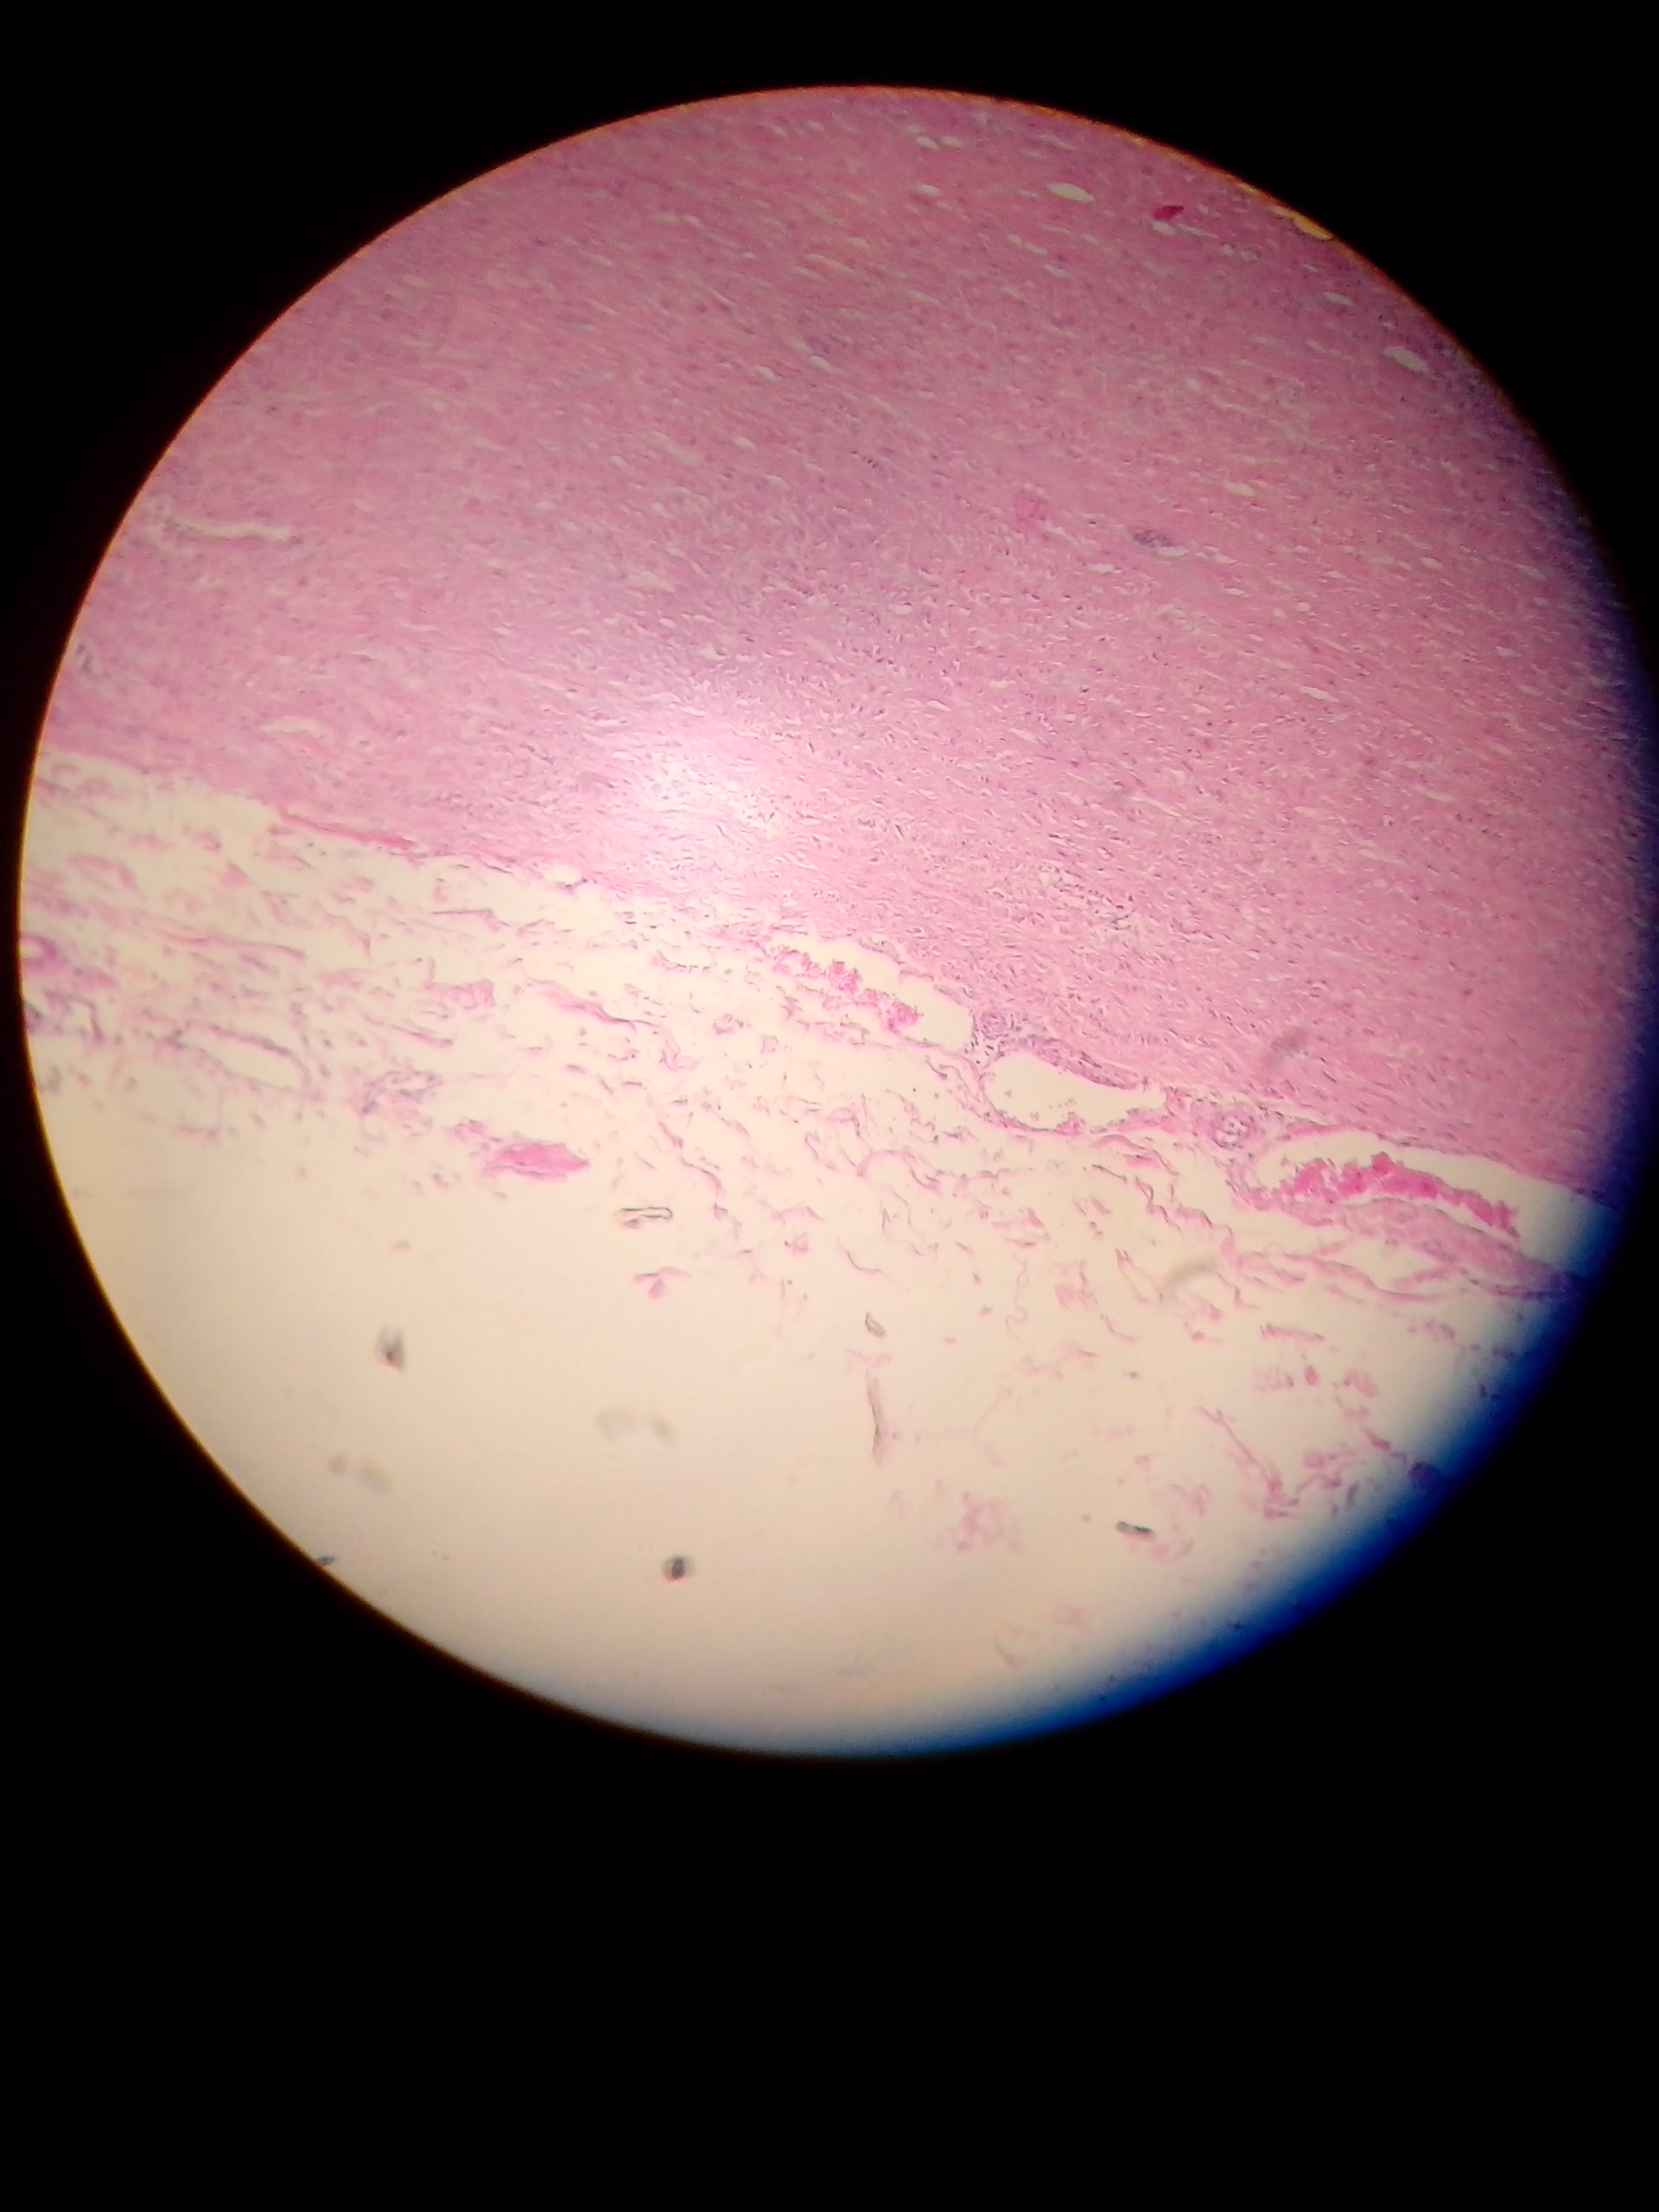
\includegraphics[angle=270, width=0.8\textwidth]{../images/01_aorta.jpg}
		\caption{Objektiv 10x}
	\caption{Aufzeichnungen der Lichtmikorskopischen Darstellungen der
		menschlichen Aorta}
\end{figure}

\subsubsection{Kommentar}

\newpage
\subsection{Blutvergleich von Mensch und Tier}

\subsubsection{Proben}
\begin{table}[h!]
	\centering
	\begin{tabular}{l l l}
		Gegenstand
			& Bezeichnung
			& Probe \\
		\hline
		Vogelblut
			& Bird Blood smear
			& 31-3134 \\
		Froschblut
			& Frog Blood smear
			& 31-3128 \\
		Menschliches Blut
			& Human Blood smear
			& 31-3152 \\
		Eigenes Blut
			& n.a.
			& n.a. \\
	\end{tabular}
\end{table}

\subsubsection{Aufzeichnungen}
\begin{figure}[h!]
	\centering
	\begin{subfigure}[b]{0.3\textwidth}
		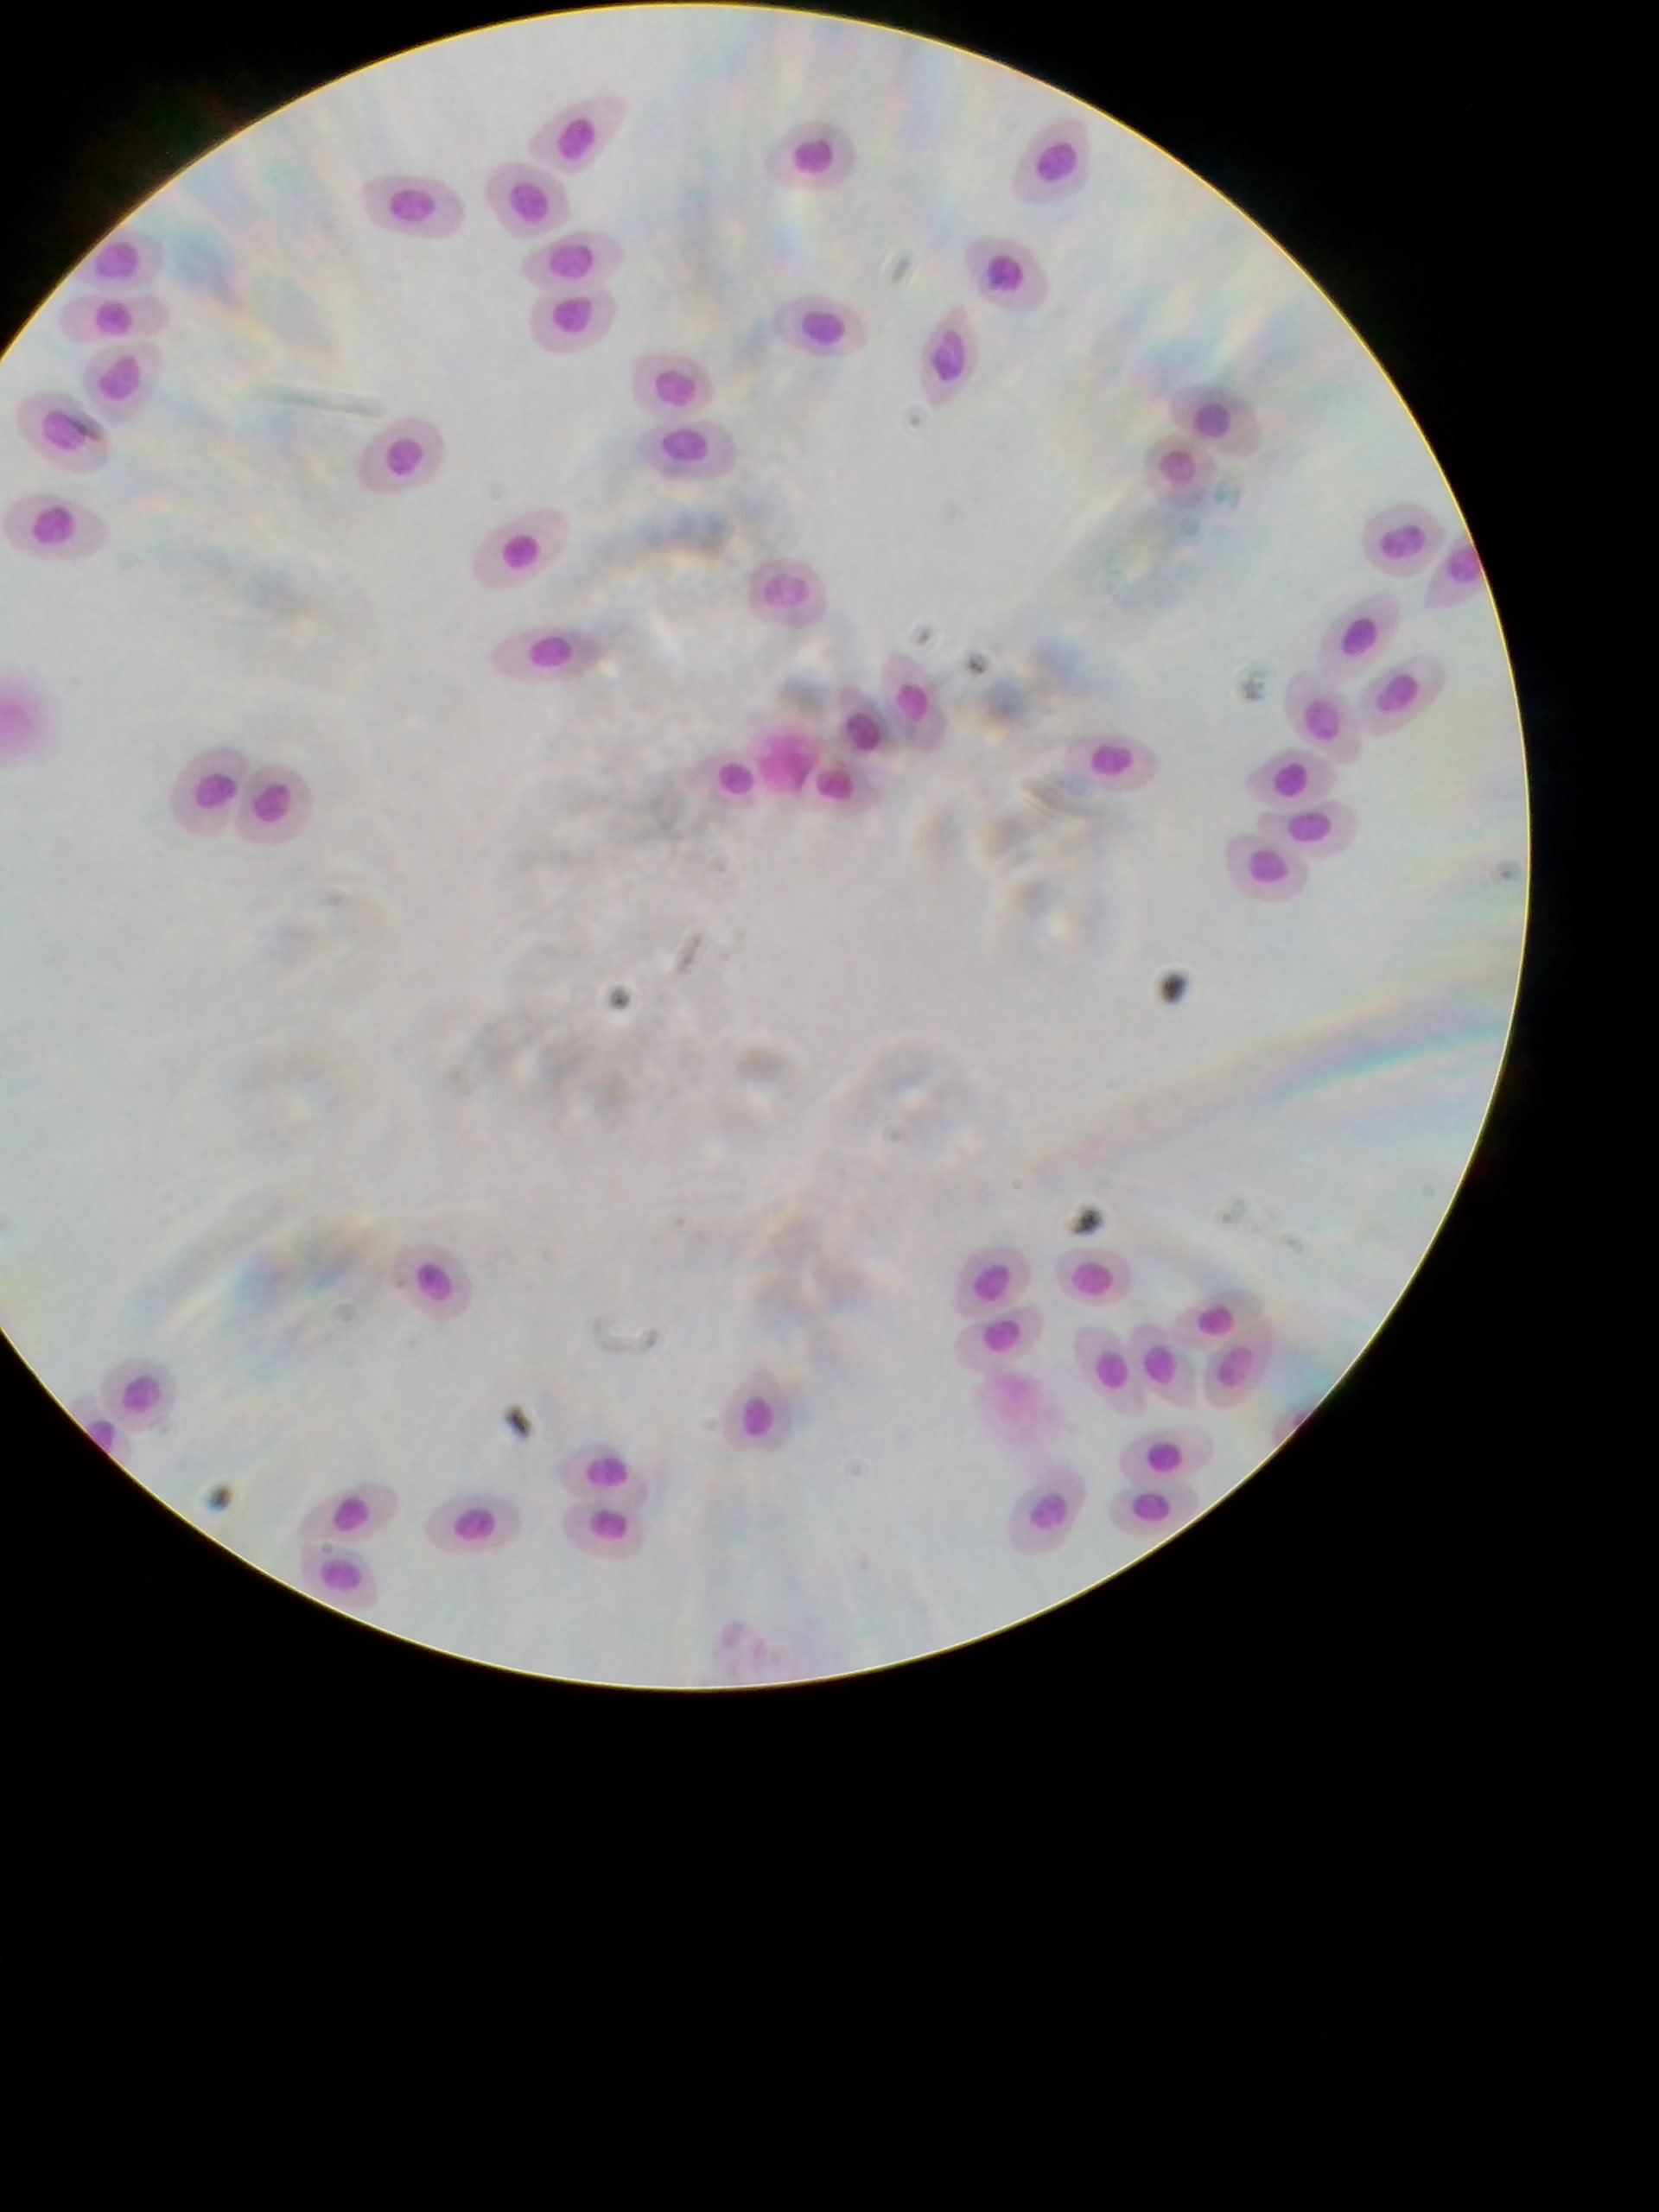
\includegraphics[width=1\textwidth]{../images/02_bird_blood.jpg}
		\caption{Vogelblut -- Objektiv 100x}
	\end{subfigure}
	\begin{subfigure}[b]{0.3\textwidth}
		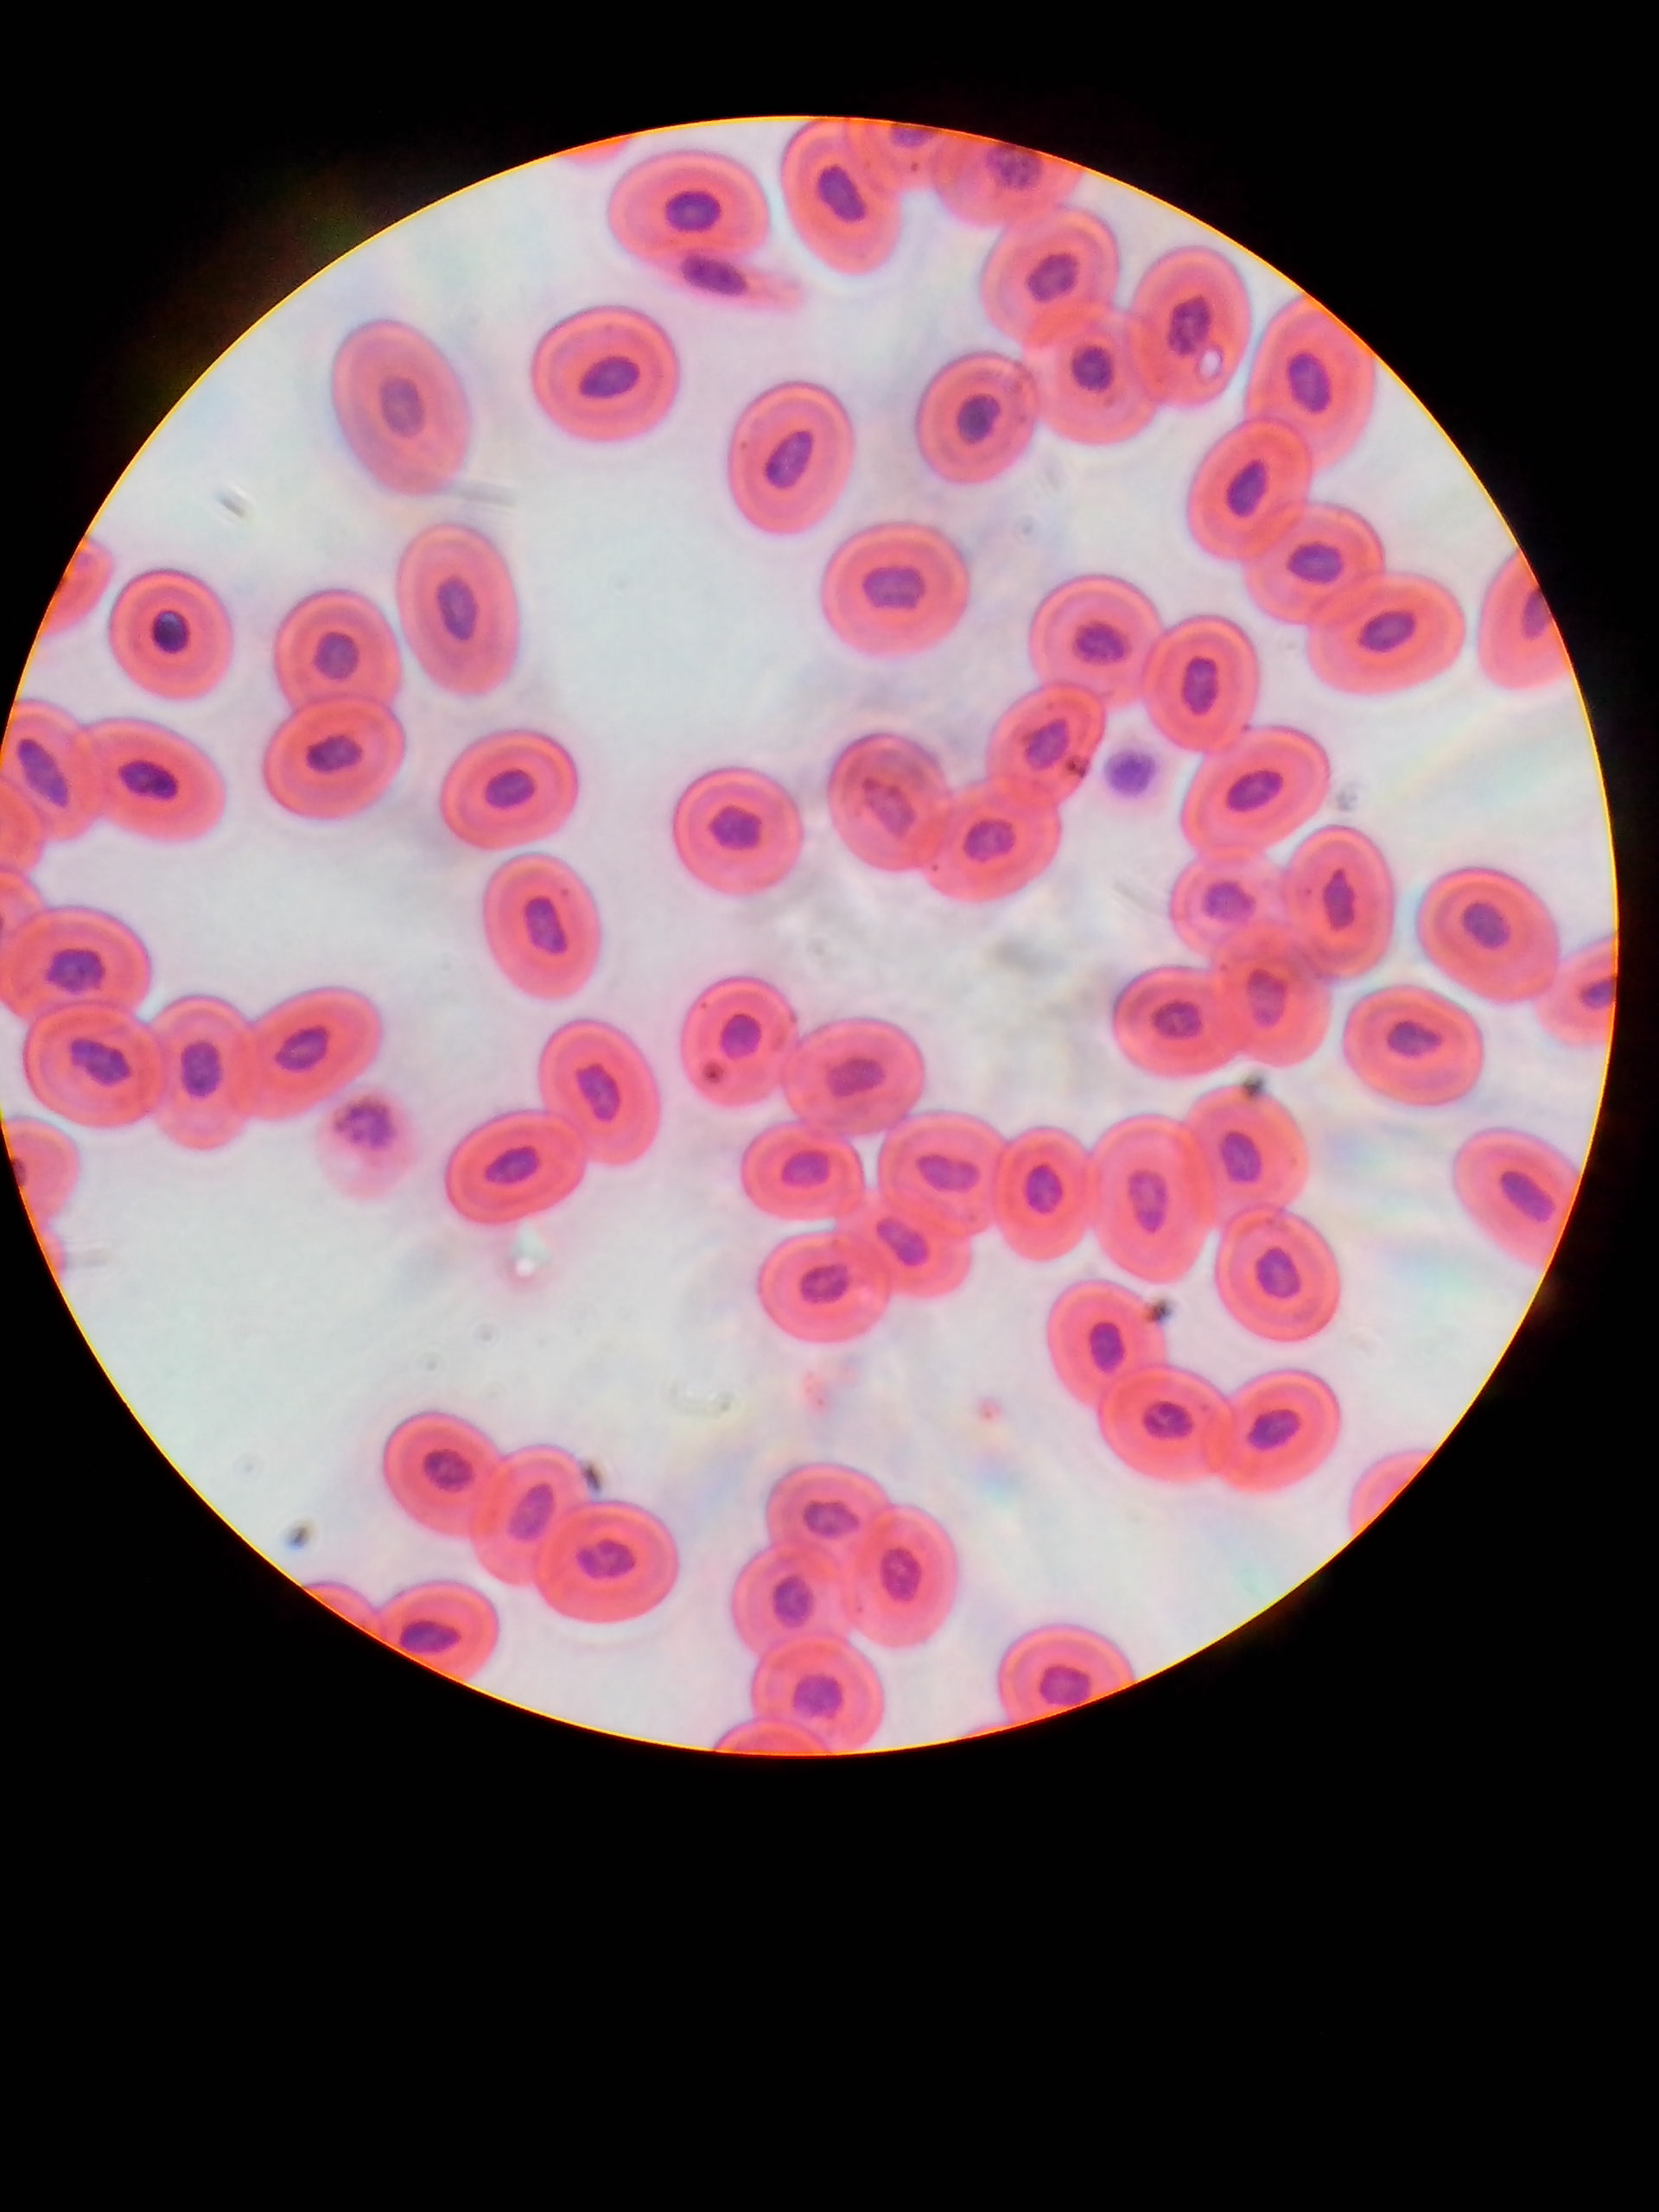
\includegraphics[width=1\textwidth]{../images/01_frog_blood.jpg}
		\caption{Vogelblut -- Objektiv 100x}
	\end{subfigure}

	\begin{subfigure}[b]{0.3\textwidth}
		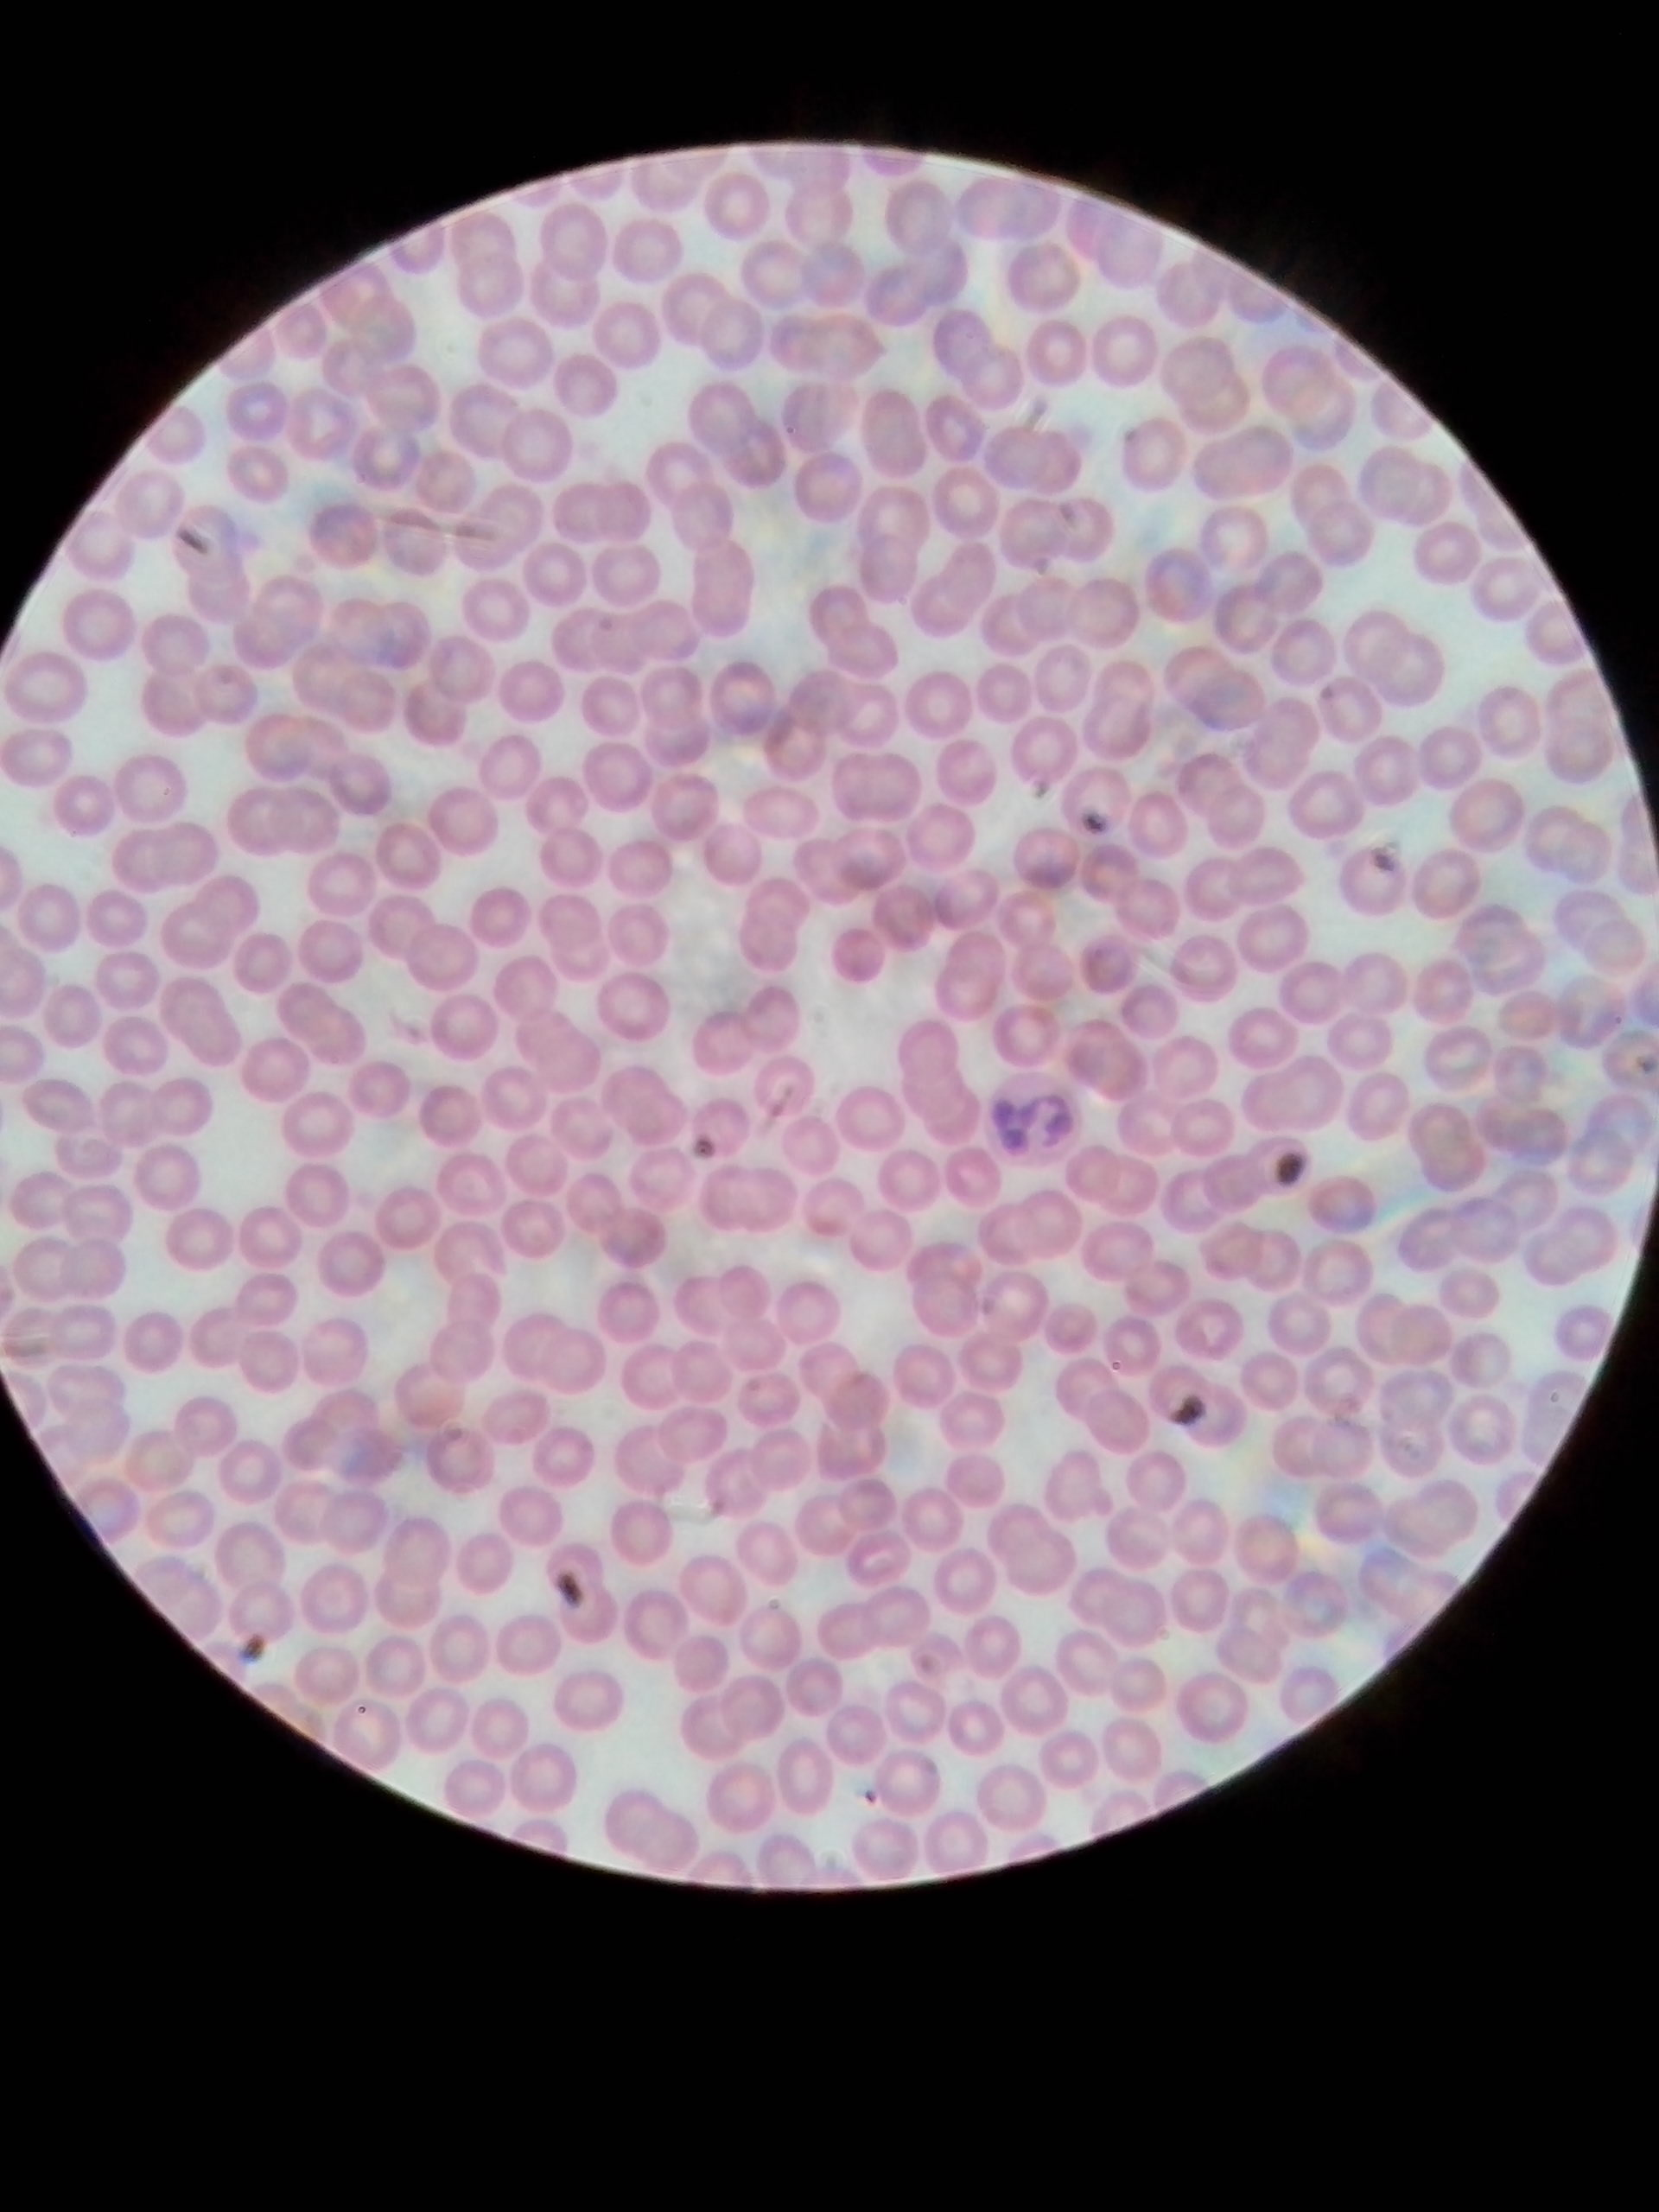
\includegraphics[width=1\textwidth]{../images/01_human_blood.jpg}
		\caption{Vogelblut -- Objektiv 100x}
	\end{subfigure}
	\begin{subfigure}[b]{0.3\textwidth}
		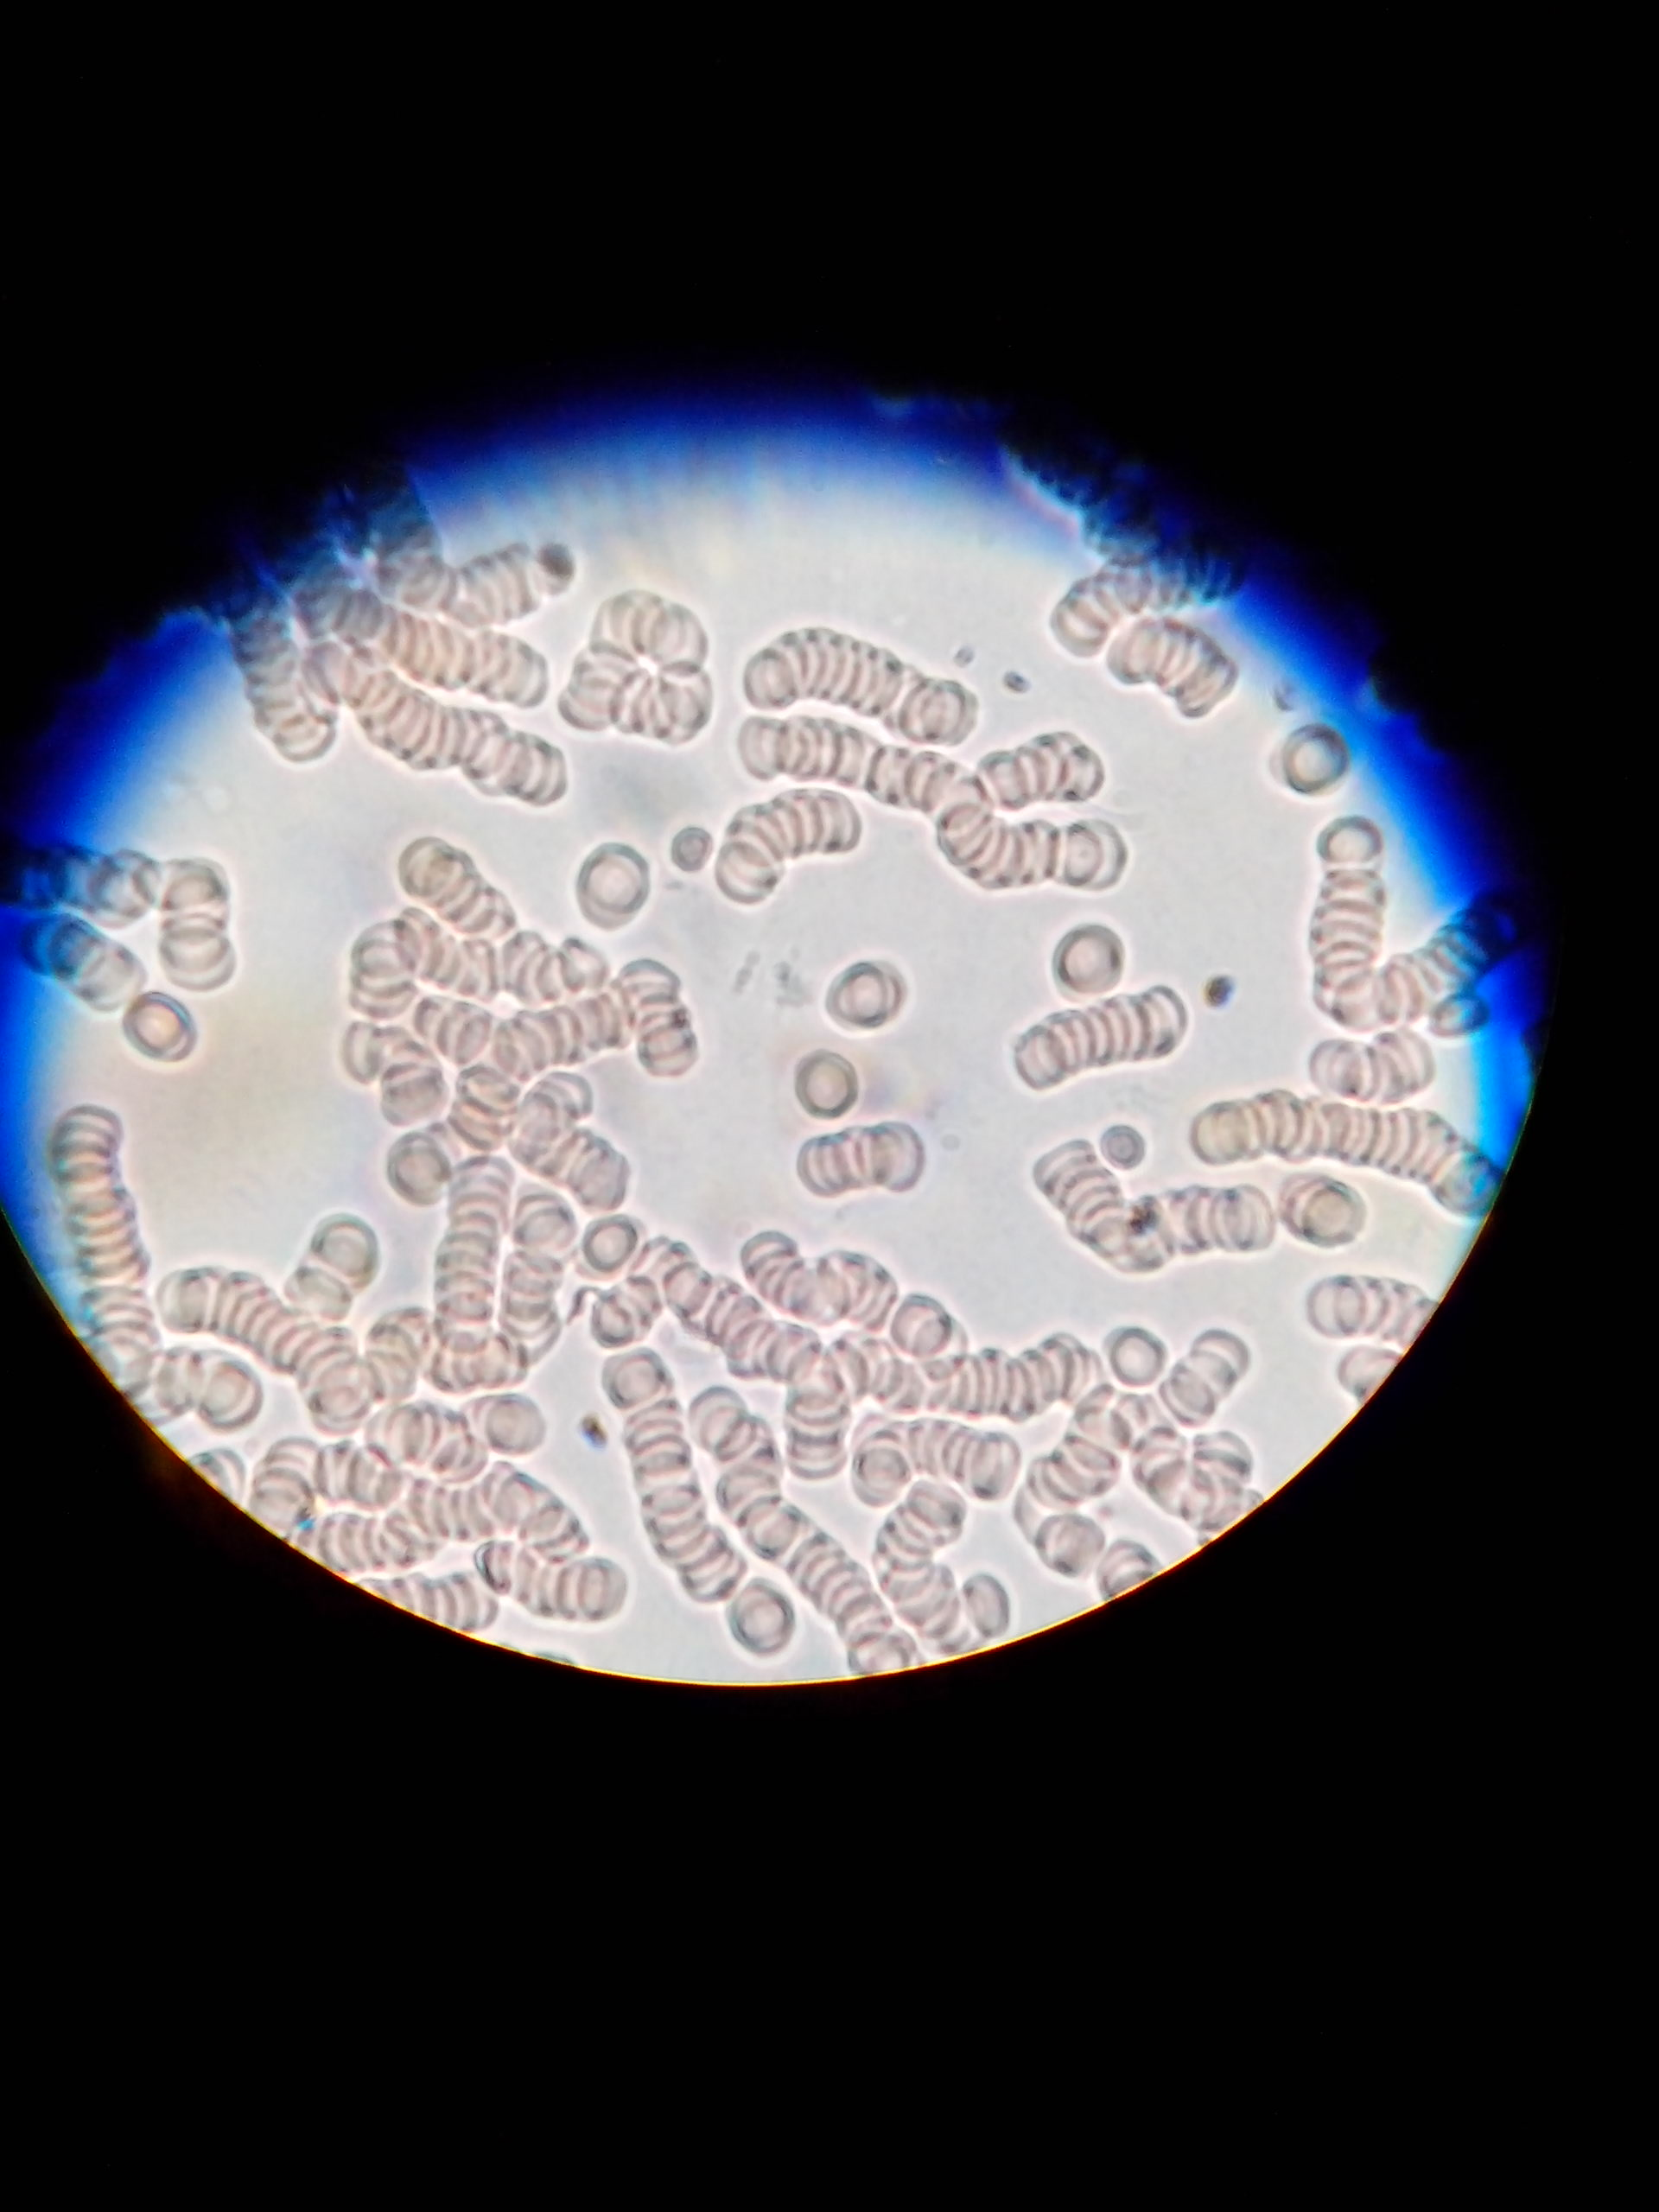
\includegraphics[width=1\textwidth]{../images/02_own_blood.jpg}
		\caption{Vogelblut -- Objektiv 100x}
	\end{subfigure}
	\caption{Autzeichnungen der Lichtmikorskopischen Darstellungen der
		verschiedenen Blutproben}
\end{figure}

\subsubsection{Kommentar}
